\documentclass[12pt]{book}
% \usepackage{times}
\usepackage{mathptmx}  % Postscript fonts for math mode
% \usepackage{fullpage}
\usepackage{amsmath}
% \usepackage{amsfonts}
\usepackage{amsthm}
\usepackage{xspace}
\usepackage{graphicx}
\usepackage{psfrag}
\usepackage{url}
\usepackage{pifont}
\usepackage{color}    % Used to highlight comments
\usepackage{geometry}
\usepackage{comment}
\usepackage{fancyvrb}
\usepackage{listings}
\usepackage{subfigure}

% Index #Raphael
\usepackage{makeidx}
\makeindex
\renewcommand\indexname{Index\label{sec:idx}}
\renewcommand\subitem{\item ~$\cdot$~}
\renewcommand\subsubitem{\item ~~~~$\cdot$~}
\renewcommand\see[2]{\!$\to$ #1}
\renewcommand\see[2]{\textit{see} #1}

% Glossary #Raphael
\usepackage{datatool}
\newenvironment{SCIONglossary}{%
  % Create new/discard old list
  \DTLifdbexists{glossary}{\DTLcleardb{glossary}}{\DTLnewdb{glossary}}
  \DTLifdbexists{abbrev}{\DTLcleardb{abbrev}}{\DTLnewdb{abbrev}}
}{%
  % Glossary.
  % Sort entries.
  \DTLsort{sortlabel}{glossary}
  \chapter{SCION Glossary}
  \begin{itemize}
    \setlength{\itemsep}{4mm}
    \DTLforeach*{glossary}%
      {\theDesc=description,\theLabel=sortlabel,\theIdx=index}{%
      \item \textbf{\theLabel~------}
      \ifx \theIdx \empty \index{\theLabel} \else \index{\theIdx} \fi
      \theDesc
    }
  \end{itemize}

  % Abbreviations.
  % Sort entries.
  \DTLsort{sortlabel}{abbrev}
  \chapter{SCION Abbreviations}
  \index{00@SCION Abbreviations}
  % Makro to prevent a line break in the first row.
  \def\newl{\relax}
  % Create table of abbreviations.
  \begin{tabular}{l|l}
    \textbf{Abbrev.} & \textbf{Description} \\
    \hline\hline
    \DTLforeach*{abbrev}%
      {\theDesc=description,\theLabel=sortlabel,\theIdx=index}{%
      \newl \theLabel & \theDesc
      \ifx \theIdx \empty \index{00@SCION Abbreviations!\theLabel} \else \index{00@SCION Abbreviations!\theIndex} \fi
      % Overwrite to achieve line breaks.
      \def\newl{\\}
    }
    \\ \hline
  \end{tabular}
  
}
% Glossary entry.
\newcommand{\gitem}[3][]{%
  \DTLnewrow{glossary}
  \DTLnewdbentry{glossary}{index}{#1}
  \DTLnewdbentry{glossary}{sortlabel}{#2}
  \DTLnewdbentry{glossary}{description}{#3}
}
% Abbreviation entry.
\newcommand{\abbrev}[3][]{%
  \DTLnewrow{abbrev}
  \DTLnewdbentry{abbrev}{index}{#1}
  \DTLnewdbentry{abbrev}{sortlabel}{#2}
  \DTLnewdbentry{abbrev}{description}{#3}
}



\usepackage{hyperref}

\newcommand{\Send}[3]{{#1}\rightarrow{#2}:&&\langle{#3}\rangle}
\newcommand{\Msg}[1]{\langle{#1}\rangle}

%% $\begin{array}{lll}
%% \Send{B}{A}{N_B, \  \mbox{MAC}_{K'_{AB}}(N_B) }\\
%% \Send{A}{B}{C_A, \ \mbox{MAC}_{K'_{AB}}(C_A||N_B)}
%% \end{array}$

\newcommand{\rpick}{{\buildrel R \over \leftarrow}}
\newcommand{\eeq}{\mathrel{{:}{:}{=}}}
\newcommand{\zo}{{\{0,1\}}}
\newcommand{\X}{{\cal X}}
\newcommand{\xor}{\oplus}
\newcommand{\qeq}{{\buildrel ? \over =}}

\newcommand{\change}[1]{\underline{\strut{\mbox{\boldmath$#1$}}}}
\newcommand{\etal}{et~al.\@\xspace} %{et~al.\@\xspace}
\newcommand{\etaltild}{et~al.\@~}
\newcommand{\eg}{e.g.,\xspace}
\newcommand{\ie}{i.e.,\xspace}
\newcommand{\MHz}{ MHz\xspace}
\newcommand{\mhz}{ MHz\xspace}
\newcommand{\io}{I/O\xspace}
\newcommand{\kbyte}{K byte\@\xspace}
\newcommand{\kbytes}{K bytes\@\xspace}
\newcommand{\kbps}{ kbps\@\xspace}
\newcommand{\TDCore}{TD Core\@\xspace}
\newcommand{\TDC}{TD Core\@\xspace}
\newcommand{\TD}{Trust Domain\@\xspace}
\newcommand{\TDs}{Trust Domains\@\xspace}
\newcommand{\AD}{AD\@\xspace}
\newcommand{\ADs}{ADs\@\xspace}
\newcommand{\PF}{Policy File\@\xspace}
\newcommand{\STUB}{Endpoint\@\xspace}
\newcommand{\TRAN}{Transit\@\xspace}
\newcommand{\RT}{Root of Trust\@\xspace}
\newcommand{\PS}{path server\@\xspace}
\newcommand{\PSs}{path servers\@\xspace}
\newcommand{\CS}{certificate server\@\xspace}
\newcommand{\CSs}{certificate servers\@\xspace}
\newcommand{\BS}{beacon server\@\xspace}
\newcommand{\BSs}{beacon servers\@\xspace}
\newcommand{\CAD}{$\textcircled{\footnotesize C}$\@\xspace}
\newcommand{\TAD}{$\textcircled{\footnotesize T}$\@\xspace}
\newcommand{\EAD}{$\textcircled{\footnotesize E}$\@\xspace}

%\newcommand{\xor}{\oplus}
%\newcommand{\zo}{{\{0,1\}}}

\hyphenation{re-pu-dia-tion}



% yih-chun/dbj hack to center text in psfrag figs
\def\centerhack#1{\hbox to 0pt{\hss\footnotesize #1\hss}}

%\newcommand{\comment}{\ding{110}\ding{43}\textcolor{red}}
\newcommand{\note}{\ding{110}\ding{43}\textcolor{red}}
\newcommand{\soobum}[1]{\ding{110}\ding{43}\textcolor{red}{Soobum: #1}}
\newcommand{\tenma}[1]{\ding{110}\ding{43}\textcolor{red}{Tenma: #1}}
\newcommand{\qi}[1]{\ding{110}\ding{43}\textcolor{red}{Qi: #1}}
\newcommand{\marknew}{\ding{110}\ding{43}\ }
\newcommand{\chris}[1]{\ding{110}\ding{43}\textcolor{red}{Chris: #1}}
\newcommand\todoRR[1]{\ding{110}\ding{43}\textcolor{red}{Raphael: #1}}

%\geometry{tmargin=.7in,bmargin=.7in,lmargin=.7in,rmargin=.7in}
\renewcommand{\baselinestretch}{0.99}

% Tighter lists
\makeatletter
\def\@listi{\leftmargin\leftmargini
    \parsep 1\p@ \@plus0\p@ \@minus\p@
    \topsep 2\p@   \@plus0\p@ \@minus\p@
%    \topsep 2\p@   \@plus2\p@ \@minus2\p@
%    \itemsep1.25\p@ \@plus\p@ \@minus\p@}
    \itemsep1\p@ \@plus0\p@ \@minus\p@}
\let\@listI\@listi\@listi
\makeatother



% float stuff
\renewcommand{\textfraction}{0}
\renewcommand{\topfraction}{1}
\renewcommand{\bottomfraction}{1}
\setcounter{totalnumber}{10}
\setcounter{topnumber}{10}
\setcounter{bottomnumber}{10}
\setcounter{dbltopnumber}{10}
\renewcommand{\floatpagefraction}{1}
\renewcommand{\dblfloatpagefraction}{1}

\newcommand{\loosenbaseline}{}%\advance\baselineskip 0pt plus 0.5pt}
\newcommand{\tightenbaseline}{}%\advance\baselineskip 0pt plus -0.5pt}




% yih-chun/dbj hack to center text in psfrag figs
\def\centerhack#1{\hbox to 0pt{\hss\footnotesize #1\hss}}
\def\dchack#1{\vbox to 0pt{\vss{\hbox to 0pt{\hss#1\hss}}\vss}}

%% Figure example
%% \begin{figure}
%%   \centering
%%   \psfrag{1}{$v_1$} % replaces "1" with $v_1$ in the figure
%%   \psfrag{2}{\centerhack{$v_2$}} % replaces "2" with $v_2$ in the figure, centered at "2"
%%   \psfrag{S0}{\dchack{\scalebox{.8}{\mbox{$v_{0}$}}}}
%%   \psfrag{M07}{\dchack{\scalebox{.8}{\mbox{$m_{07}$}}}}
%%   \includegraphics[width=.7\columnwidth]{mht2} % includes figure mht2.eps
%%   \caption{Tree authenticated values}
%%   \label{fig:basic-mht}
%% \end{figure}


\title{
  --- The Official SCION Manual --- \\
  {\large Design, Implementation, Applications, Tools}
}
\author{
  The SCION Team\\
  (ETH Zurich, Carnegie Mellon University)
}
\date{\today}




\begin{document}

  \pagenumbering{roman}
  \maketitle
  \vspace{20mm}
  \abstract

This document describes the essential components of the V1.0 SCION
prototype including functional specifications of the SCION network
elements (e.g., servers, routers, gateways), data structures of
configuration files, and communication protocols among these
elements. In particular, this document focuses on the specification
of a working prototype and additional features that are not described
in the academic papers~\cite{ZHHCPA2011}.

This is a working document which will be continuously updated during
the prototype creation process. It includes discussions or comments
on current design issues.




  \newpage
  \tableofcontents

  \newpage
  \pagenumbering{arabic}
  \setcounter{page}{1}
  \section{Introduction}
We first describe the design principles of SCION and 
based on these design principles, we describe SCION implementation in detail.

  
\abstract

This document describes the essential components of our V1.0 SCION prototype which
includes functional specifications of SCION network elements (e.g., servers,
routers, gateways), data structures of configuration files, and communication protocols among
these elements. In particular, this document focuses on the
specification of a working prototype and additional features that are not
described in the original paper. This is a working document which will be continuously updated
during the prototype creation process and includes discussions or comments on
current design issues. This document is written under the assumption that the original
SCION paper is read and understood in detail~\cite{ZHHCPA2011}.

\section{Introduction}

\subsection{SCION Overview}

SCION (Scalability, Control, and Isolation On Next-generation networks) is a
clean-slate Internet architecture designed to provide route control, failure
isolation, and explicit trust information for end-to-end communication. SCION
separates Autonomous Domains (ADs)\footnote{We use the term AD instead of AS to
  denote a smaller unit -- large domains with geographically dispersed units may
  constitute a single AS, however, we would consider them as multiple ADs.} into
groups of independent routing sub-planes, called trust domains (TDs), which then
interconnect for global connectivity. Trust domains provide natural isolation
for routing failures and human misconfiguration, give endpoints strong control
for both inbound and outbound traffic, provide meaningful and enforceable trust,
and enable scalable routing updates with high path freshness. As a result, SCION
provides strong resilience and security properties as an intrinsic consequence
of first-class security design principles, avoiding piecemeal add-on protocols
as security patches. Meanwhile, SCION only assumes that a few top-tier ISPs in
the trust domain are trusted for providing reliable end-to-end communications,
thus achieving a small Trusted Computing Base (TCB). Both our security analysis
and evaluation results show that SCION naturally prevents numerous attacks and
provides a high level of resilience, scalability, control, and isolation. A
high-level SCION architecture is illustrated in Figure~\ref{fig:overview}.

\begin{figure*}[ht]
\centering
\includegraphics[width=.9\columnwidth]{./fig/overview.eps}
\caption{SCION Architecture.}\label{fig:overview}
\end{figure*}

We can summarize the design principles of SCION as follows.
\begin{enumerate}
\item {\bf Domain-based isolation.} Dividing the routing control plane into
  independent domains. Isolation among independent domains protects routing in
  one domain from malicious activities and routing churn in other domains. This
  benefits both security and scalability while retaining reachability and path
  diversity across domains. For example, SCION enables frequent routing updates
  to periodically refresh path state, so that each AD always maintains a fresh
  (and accurate) network topology for efficient routing decisions. This
  separation also enables a separate root of trust for each domain, avoiding the
  conundrum of having to select a universally trusted single global root of
  trust. Finally, such isolation enables \textit{enforceable accountability},
  which enables punishment in case of misbehavior. In the current Internet,
  accountability is of limited utility as there is often no enforceability to
  handle detected misbehavior. By separating domains with enforceable
  accountability from domains without enforceability we can prioritize traffic
  accordingly and sidestep a major quagmire in the current Internet of how to
  prioritize traffic in case of DDoS attacks.
\item {\bf Mutually controllable path selection.} Joint path selection between
  source and destination. SCION greatly increases both the source and
  destination’s ability to affect, select and control the construction of the
  routes to and from themselves, while still respecting intermediate ISPs’
  routing policies.
\item {\bf Explicit trust and small TCB for end-to-end communication.} By
  segregating mutually distrustful entities into different trust domains, each
  trust domain can choose a coherent root of trust (e.g., a few tier-1 ISPs) for
  bootstrapping trust among ADs in the same trust domain. As a result, an
  endpoint E knows and is able to choose explicitly whom to trust for achieving
  reliable end-to-end communication, while untrusted ADs in other trust domains
  cannot affect the path discovery and route computation of E. Consequently, an
  entity only has to trust a small subset of the network thus achieving a small
  TCB for end-to-end communication.
\end{enumerate}


We briefly describe the end-to-end path construction in SCION and necessary functions for network elements. Furthermore, we introduce three servers, which help satisfy the design principles listed above.
\begin{itemize}
\item {\bf Path Construction. } A \TDC starts propagating a Path Construction
  Beacon (PCB) to construct a path. PCB initiation is performed by {\bf Beacon
    Servers} in the \TDC -- \BSs in the \TDC generate a PCB
  periodically. For PCB propagation, \BSs in an \AD send PCBs to
  \BSs in neighboring domains -- \BSs in \TRAN \ADs
  propagate the PCB received from their parent \AD to their customer \ADs. A
  \BS adds its own \AD information (i.e., Opaque Field, digital
  signature, etc.) to the PCB. For signature verification, the \BS
  needs the public keys of the \AD who previously signed the PCB. The public key
  of each \AD is provided by the {\bf Certificate Server}, which stores the
  certificates of \ADs and provides \ADs' public keys to the \BS or
  the certificates to its customer \ADs when requested. When a border router
  receives a PCB, it forwards it to all \BSs within the \AD. Hence,
  for beacon propagation, border routers only need to know the \BSs
  within their own AD. The certificate server keeps track of all server
  locations (i.e., \BSs, certificate servers, and path servers as
  described below) and notifies to border routers of any topology change within
  the \AD.

\item {\bf Path Registration. } Once an \STUB \AD receives a PCB, it selects $k$
  paths to use and registers them with the {\bf Path Server} in the \TDC. The \TDC \PS
  processes path registration requests (e.g., whether to accept or reject) and
  stores this $k$ path registration information of the \STUB \AD.

\item {\bf End-to-end Path Resolution. }  A source \AD constructs a path to
  reach a destination \AD by composing its path to the \TDC (up-path) with the
  path from the \TDC to the destination \AD (down-path). To this end, when the
  \BS of an \AD receives a PCB, it provides the corresponding up-path (note that
  a PCB contains a path to the \TDC) to {\em local} path servers. Local path
  servers store up-paths and provide them to endhosts. Meanwhile, down-paths are
  acquired from the \TDC path server that holds $k$ down-paths to each \AD. The
  local path server sends path queries on behalf of endhosts and caches the
  results for later queries. The path server location is registered with the
  certificate server. A \BS extracts new paths to \TDC from received PCBs and
  sends them to local path servers. Note that ADs can have multiple path servers
  for load balancing, as well as multiple path, certificate, and beacon servers
  for reliability.

\item {\bf Packet Forwarding. } Border routers distinguish two packet types:
  control and data packets. They forward control packets internally to the
  corresponding services; and forward data packets directly to egress interfaces
  (or hosts if the packet destination is within its \AD) specified in the packet
  header as an \textit{opaque field}. Since routers forward packets using the
  opaque fields in the packet header, they do not need to keep any forwarding
  table nor compute routes.
\end{itemize}

\subsubsection{\TD: Root of Trust}

A \TD is an independent {trust} network whose members reside in a common
contractual, legal, or regional environment. We envision \TDs to grow to a
region where all internal \ADs can agree on a common root of trust, and where
accountability can be enforced on all internal \ADs. A \TD consists of many \ADs
with various roles. \TDC \ADs, which are generally big, national ISPs, provide
service to small ISPs (e.g., regional ISPs) or directly to \STUB \ADs (e.g.,
companies, universities). In principle, a \TD needs at least one \TDC \AD for
\TD management and path construction. \TRAN \ADs provide network connectivity to
\TDC for customer \ADs and/or manage peering relationships with other \TRAN \ADs
(i.e., shortcuts) for improved service (in terms of path quality; e.g., path
length, path bandwidth). \STUB \ADs directly connect to endhosts and provide
domain resolution service (i.e., domain to path translation service) to those
hosts. Naturally, each \AD trusts its provider \AD(s), and as a consequence all
\ADs trust the \TDC. Hence, all \STUB \ADs in the same \TD trust each other by
trusting the \TDC -- the Root of Trust -- without establishing individual trust
relationships. The Root of Trust is established by an agreement among \TDC \ADs
and specified in the Root of Trust file (viz., Section~\ref{subsec:root-of-trust}).

\subsubsection{Autonomous Domain}
Each \AD provides the following services based on its type.
\begin{itemize}
\item {\bf \TDC \AD: } \TD membership service (both for \TDC members and non-\TDC members), certificate service (AD certificate issue/reference), PCB initiation, path record (i.e., handling path registration from \STUB \ADs), and domain resolution (i.e., domain to path translation).
\item {\bf \TRAN \AD: } certificate service (reference only), PCB propagation, path selection and registration (for endhosts), domain resolution.
\item {\bf \STUB \AD: } path selection and registration (for endhosts), domain resolution. 
\end{itemize}

\noindent{\bf Common services: } certificate management for internal entities (e.g., router, switch, server), up-path (to \TDC) resolution service, topology management (external: border router to neighbor AD map, internal topology: server location), key management (offline key, online key), 

\subsubsection{Servers}
To facilitate efficient routing, each \AD runs three servers. The required services at \TDC \AD, \TRAN \AD, and \STUB \AD are annotated by \CAD, \TAD, and \EAD, respectively. Internal services and external services indicate those services provided within an \AD and across \ADs, respectively.
%\begin{itemize}

\noindent{\bf Certificate Server: } 
\begin{itemize}
\item \AD certificate service: respond to certificate requests (\CAD, \TAD,\EAD) 
\item \AD certificate management: issue certificate(\CAD), store certificates (\CAD,\TAD,\EAD)
\item Entity certificate service/management: certificates of internal entities (\CAD,\TAD,\EAD)  
\item Key management: manage the secret key for internal secure communication (\CAD,\TAD,\EAD), generate/distribute opaque field generation (OFG) key (\CAD,\TAD,\EAD) 
\item Topology management: distribute internal server locations to border routers (all external messages are forwarded to the corresponding servers by border routers, without revealing server locations outside the \AD.) (\CAD,\TAD,\EAD), manage database of border router (interface) to \AD mapping
\end{itemize}

\noindent{\bf Beacon Server: }
\begin{itemize}
\item PCB generation: initiate a PCB for path construction (\CAD)
\item PCB propagation: gather all PCBs arrived from provider \ADs, select $k$ PCBs (for every PCB propagation period), propagate selected PCBs to customer \ADs (\TAD)
\item path selection/registration: select $k$ down-paths from \TDC and register them to the \TDC path server (\TAD,\EAD)
\item path distribution: distribute up-paths to path servers (\TAD,\EAD) 
\end{itemize}

\noindent{\bf Path Server: }
\begin{itemize}
\item path record: keep $k$ down-paths for each \AD within a \TD (\TAD)
\item domain resolution: translate the identifier of a destination \AD to the down-path(s) (i.e., from the \TDC to the \AD) (\CAD,\TAD,\EAD) (\TAD,\EAD resolve a path either by sending a query to the \TDC path server or using cached results) 
\item path caching: cache down-paths to destination \ADs and up-paths to \TDC (\TAD,\EAD)
\end{itemize}


\subsection{Implementation Principles}
The SCION architecture and implementation are guided by the following principles:

\begin{enumerate}
\item {\bf Simple Router. }
Routers run with very simple functions: forwarding without per-flow and per-destination state, and efficient path verification.
%SCION edge routers forward all PCBs to the Beacon Server
%No huge routing table and forwarding table

%No complex route selection policies

\item {\bf Simple Configuration. }
An \AD should be able to add and configure routers easily. Complex configuration
can lead to outages or limited availability.

%Border routers need to know ``Keys'' and ``Server location''

\item {\bf Efficient Forwarding. }
The basic function (i.e., packet forwarding) of a router should be fast enough to operate at a line speed. It is desirable for routers to forward packets in $O(1)$ time (i.e., to remove any dependency on other factors such as the forwarding table size). 
%No FIB lookup
%A single hash operation

\item {\bf Scalability. }
Path advertisement and construction should be scalable to easily accommodate ever growing network size. For scalability, it is desirable to minimize any state that need to be kept at individual routers (or servers).

\item {\bf Rebootability. } The Internet should be able to reach a globally
  stable state when some or all network elements restart. In essence,
  rebootability means that no circular dependencies exist that would lead to a
  deadlock when a network is ``rebooted.''

\item {\bf Clean Trust Model. } The root of trust should be easily set up and
  the flow of trust should be {\em explicit}, such that the TCB for each network
  operation can be simply enumerated.

\end{enumerate}

%Outcomes: Highly resilient Internet architecture that can be incrementally deployed besides the current IP protocols. SCION will provide strong availability and reliability guarantees for a variety of traffic classes. 

%No global route advertisement

%No routing table management

%\end{itemize}

%\subsection{Bootstrapping}

  \chapter{Certificate Server}
A \CS manages its own AD certificate issued by \ISDC and the
certificates of all entities within an \AD, and handles certificate
requests. In addition, a \ISDC certificate server manages the \RT file
on which all entities within an \ISD establish {trust}. A \CS contains
a key server, which generates and distributes keys for securing
internal (i.e., intra-AD) communication.

\section{Root of Trust File} \label{subsec:root-of-trust}
The \RT file contains the list of all \ISDC members and their
signatures. The file keeps track of the current policy number and the
\ADs that signed the policy. The policy is used as a {\bf \em root of
trust} by which all \ADs in the ISD establish their trust. The notion
of root of trust is crucial in the SCION architecture due to the
hierarchical structure of the \ISD. As a consequence, the ISD
membership is strictly limited and agreed by the current members.
This is enforced by restricting the update privilege of the \PF. More
specifically, the current members of \ISDC define the minimum number
of \ADs that should provide their signature for updating the \RT file
-- defined as {\em Policy Quorum Threshold} ($P_{th}$). Furthermore,
the \ISDC members define the minimum number of \AD signatures to grant
a new \AD's joining to the \ISDC and to issue a certificate for the
AD. This number, defined as {\em Certificate Quorum Threshold}
($C_{th}$), is also included in the \PF. Hence, an \AD, if it is
approved to join a \ISDC, would be included in the \RT file that is
signed by at least $C_{th}$ \ISDC \ADs. Figure~\ref{fig:rot-file}
shows the contents of the \RT file constructed in the XML format.

\begin{SaveVerbatim}{RotSection}
<ROT>
	<header> 
	<!-- Why we just switch this header field to ROT header properties -->
		<policyNumber>"policyNumber"</policyNumber>
		<ISDID>"Isolation Domain ID"</ISDID>
		<policyThreshold>"policyThreshold"</policyThreshold>
		<certificateThreshold>"certificateThreshold"</certificateThreshold>
	</header>
	<coreADs>
		<coreAD>
			<AID>"AID"</AID>
			<publicKey>"publicKey"</publicKey>
		</coreAD>
		...
	</coreADs>
	<signatures>
		<coreAD>
			<AID>"AID"</AID>
			<sign>"Signature"</sign>
		</coreAD>
		...
	</signatures>
</ROT>
\end{SaveVerbatim}

\begin{figure}[h]
\centering
%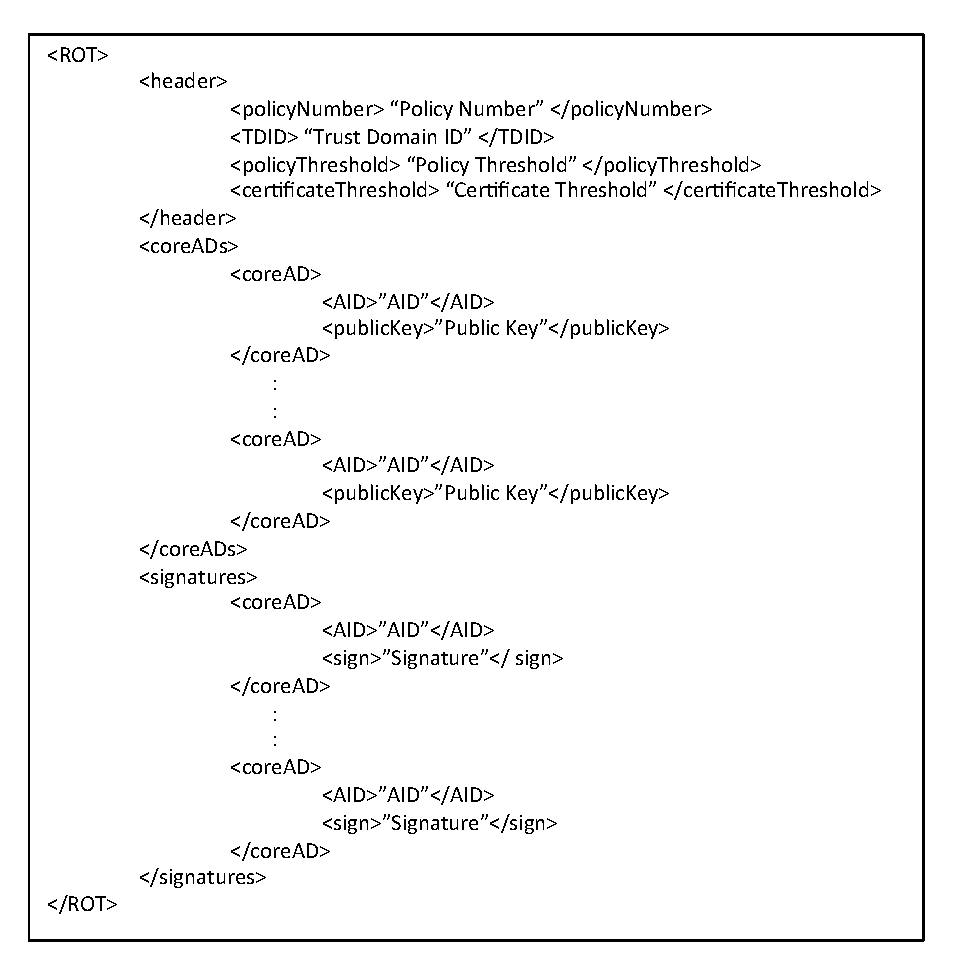
\includegraphics[width=.7\columnwidth]{./fig/rotfile.eps}
%\caption{\RT File Format}\label{fig:rot-file}
\begin{center}
	\fbox{
		\begin{minipage}{\columnwidth}
			\BUseVerbatim[fontsize=\footnotesize]{RotSection}
		\end{minipage}
	}
\end{center}
\caption{\RT File Format}\label{fig:rot-file}
\end{figure}

\tenma{We can define DTD (Document Type Definition) for XML structure.}

\paragraph{Header}
The header contains the \ISDC policy information listed below. 

\begin{enumerate}
\item Isolation Domain ID (ISD ID or TID) : Globally unique Isolation Domain identifier.
\item Policy ID : Current version number of \PF.
\item Policy Quorum Threshold : Minimum number of \ISDC \ADs needed to generate a new \RT file. 
\item Certificate Quorum Threshold : Minimum number of \ISDC \ADs needed to issue a new certificate for an \AD.
\end{enumerate}
\tenma{Should we keep a timestamp field or identifier to distinguish the difference of versions?}

\paragraph{\ISDC member list}
The \ISDC member list contains the information of all \ISDC members. Each \AD has the following elements:
\begin{enumerate}
\item \AD ID (AID).
\item \AD's public key.
\end{enumerate}

\paragraph{Signatures}
The signatures element contains the signatures of the \ISDC ADs that signed the current \RT file.
\begin{enumerate}
\item AD ID (AID).
\item \AD's signature computed over the header and the \ISDC member list.
\end{enumerate}

\tenma{Updating RoT files is also needed to included since certificate would be expired or revoked
in some conditiona.}

\section{Certificate Management} 

\begin{figure*}[ht]
\centering
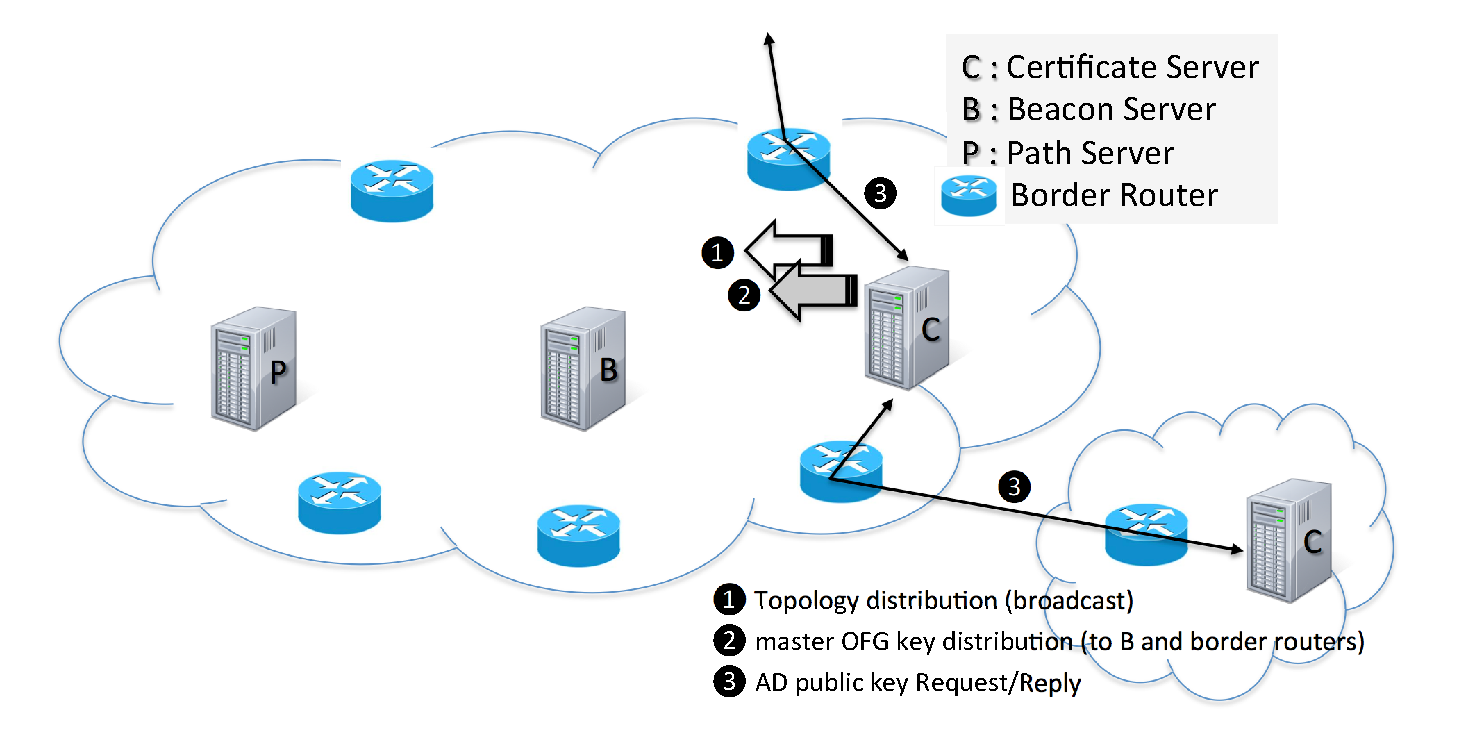
\includegraphics[width=.9\columnwidth]{./fig/cs_message.eps}
\caption{Certificate Server messages.}\label{fig:cs-message}
\end{figure*}

\noindent{\bf AD certificate: } The certificates of all participating \ADs to an \ISD are issued by the certificate authority of \ISD and stored at \ISDC \ADs and the owner of the certificates. Certificate servers are responsible for managing a certificate database and providing certificates to requesting \ADs. An \AD certificate contains the public key of an \AD signed by the \ISD's certificate authority. An \AD, using \AD certificates, verifies the signatures of other \ADs in inter-\AD communication (e.g., PCBs signed by its providers).

The {\em \ISDC certificate server} holds all certificates of \ADs that belong to the \ISD and provides them to requesting \ADs. Only certificate servers are allowed to request \AD certificates and for the request, they need to provide their signature for the request. A certificate request cannot be directly made to \ISDC certificate server, yet should traverse all \CSs on the path to \ISDC. For example, when a \STUB \AD requests an \AD's certificate (to \ISDC), this request is forwarded to the \CS of its provider \AD. Border routers can forward the request to the \CS (by putting the server address to the destination AID field) since they keep track of the server locations; viz., topology distribution below. The provider's \CS immediately responds to the request if the requested certificate is present in its local cache (or database) or (2) requests the certificate to its provider \AD. This procedure continues recursively up to \ISDC, until the certificate is found and returned to the requester. The \CSs on the return path store the certificate so that they respond to any later request for  the same certificate immediately. 
\tenma{This part is similar to how DNS query works. For Certificate request message, should the Endpoint AD puts its signature for identity
verification? even if it just requests the ``public'' informaiton, i.e., certificate.}

\noindent{\bf Entity certificate: } An \AD's \CS holds the certificates of all local entities such as routers, switches, servers, and gateways to secure intra-\AD communication. When an entity is added to an \AD, the entity is issued an certificate from the local certificate authority and register the certificate to the \CS. All border routers are configured to keep the \CS certificate of its own \AD to authenticate the messages from the \CS. Note that the border routers keep updated with the Opaque Field Generation (OFG) key and server list (in the topology file) by the \CS.


\section{Key Management}
A \CS shares a (master) secret key with each entity (server, router, or gateway) in the \AD, with which the \CS establishes a secure channel with those entities. The master secret key is pre-installed at individual entities when they join the \AD\tenma{Why we just use pre-installed certificate instead of using master secret key. Using symmetric cryptographic based on master secret may cause some problems}. The \CS generates a OFG key periodically (e.g., once a day) and distributes it to the \BS and border routers\tenma{securely? using authenticated-encryption based on the master secret key or envelope secure message based on asymmetric cryptography?}. Using this OFG key, the \BS creates PCBs (more specifically, opaque fields in PCBs) and the border routers verify the opaque fields. 

\begin{itemize}
\item {Offline Key: } master secret key
\item {Online Key: } OFG key
\end{itemize}



\section{Topology}
A \CS maintains the \AD topology file that describes the list of entities and their configuration information.
All entities are assigned a unique AID and type. The entity types currently defined in SCION and the information that need to be specified by each type are as follows.
AID is the authenticated ID of an entity and is used for an address identifier \chris{AID is also the abbreviation for AD ID and is used in \RT file, this is a bit confusing}; and the type identifier is specified in the parenthesis.

\begin{itemize}
\item Certificate Server (TYPE\_CS): AID \tenma{AID are same for different entities, such as Cert, Beacon, Path Servers? Here they look the same. My suggestion is using some real instances to describe it in Figure~4.}
\item Beacon Server (TYPE\_BS): AID
\item Path Server (TYPE\_PS): AID
\item Border Router (TYPE\_BR): AID, interface ID, neighbor \AD (AD ID), \AD relationship (P,C,E)\newline
	* P:Provider, C:Customer, E:pEer
\item Gateway (TYPE\_GW): AID, protocol 
\end{itemize}
Each interface card in a border router is assigned a unique interface ID among all interfaces within an AD to expedite packet forwarding. That is, an ingress router, on receiving a packet, forwards the packet directly to the egress router and the egress router sends out the packet to the interface ID specified in the packet. The information regarding the interface ID to neighbor \AD mapping and \AD relationship is used by the \BS when the \BS makes a PCB propagation decision (e.g., which PCB to propagate to which \AD). Furthermore, neighbor \AD can be used for internal traffic engineering (e.g., \AD-level bandwidth allocation and enforcement). A gateway is used to connect a SCION network to a heterogeneous network that runs with a different protocol (e.g., IPv4, IPv6). 
The \AD topology is stored in XML format as shown in Figure~\ref{fig:topology-file}.

%\begin{figure}[h]
%\centering
%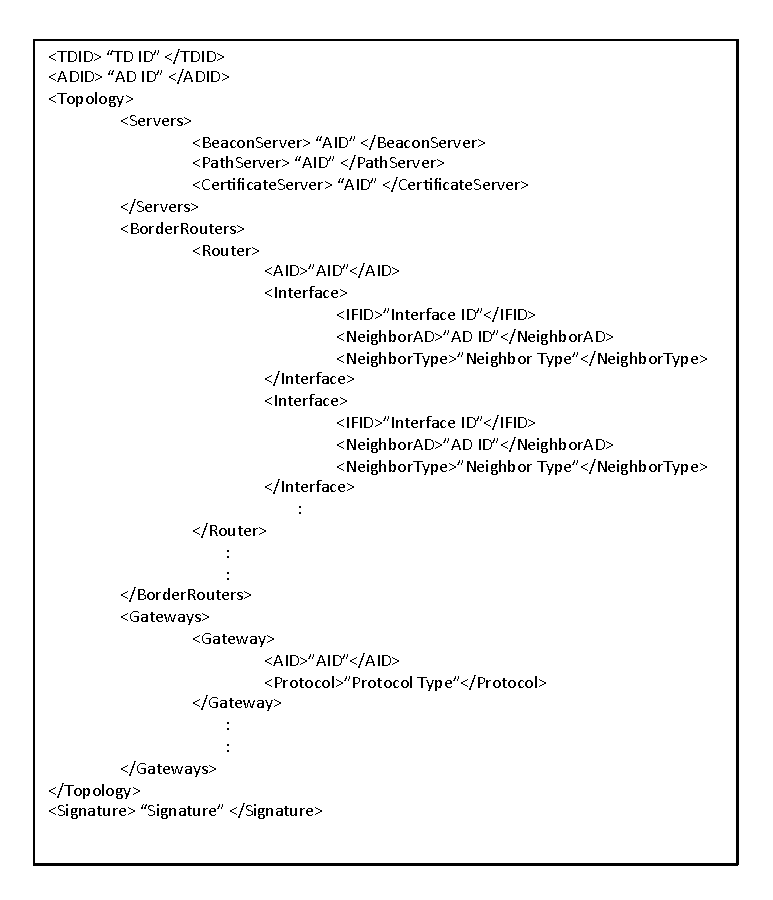
\includegraphics[width=.7\columnwidth]{./fig/topologyfile.eps}
%\caption{Topology File Format}\label{fig:topology-file}
%\end{figure}

\begin{SaveVerbatim}{TopSection}
<Topology ISDID="ISD ID" ADID="AD ID">	
<!-- put ISDID and ADID here beacuse a valid xml only has one root element -->
	<Servers>
		<BeaconServer>"AID"</BeaconServer>
		<PathServer>"AID"</PathServer>
		<CertificateServer>"AID"</CertificateServer>
	</Servers>
	<BorderRouters>
		<Router>	
		<!-- Why we just switch single field to property header -->
			<AID>"AID"</AID>
			<Interface>
				<IFID></IFID>
				<NeighborAD>"AD ID"</NeighborAD>
				<NeighborType>"AD ID"</NeighborType>
			</Interface>
			<Interface>
				<IFID></IFID>
				<NeighborAD>"AD ID"</NeighborAD>
				<NeighborType>"AD ID"</NeighborType>
			</Interface>
				...
		</Router>
		<Router>
			...
		</Router>
			....
	</BorderRouters>
	<Gateways>
		<Gateway>
			<AID>"AID"<AID>
			<Protocol>"Protocol Type"</Protocol>
		</Gateway>
			...
	</Gateways>
	<Signature>"Signature"<Signature>
</Topology>
\end{SaveVerbatim}

\begin{figure}[h]
\centering
%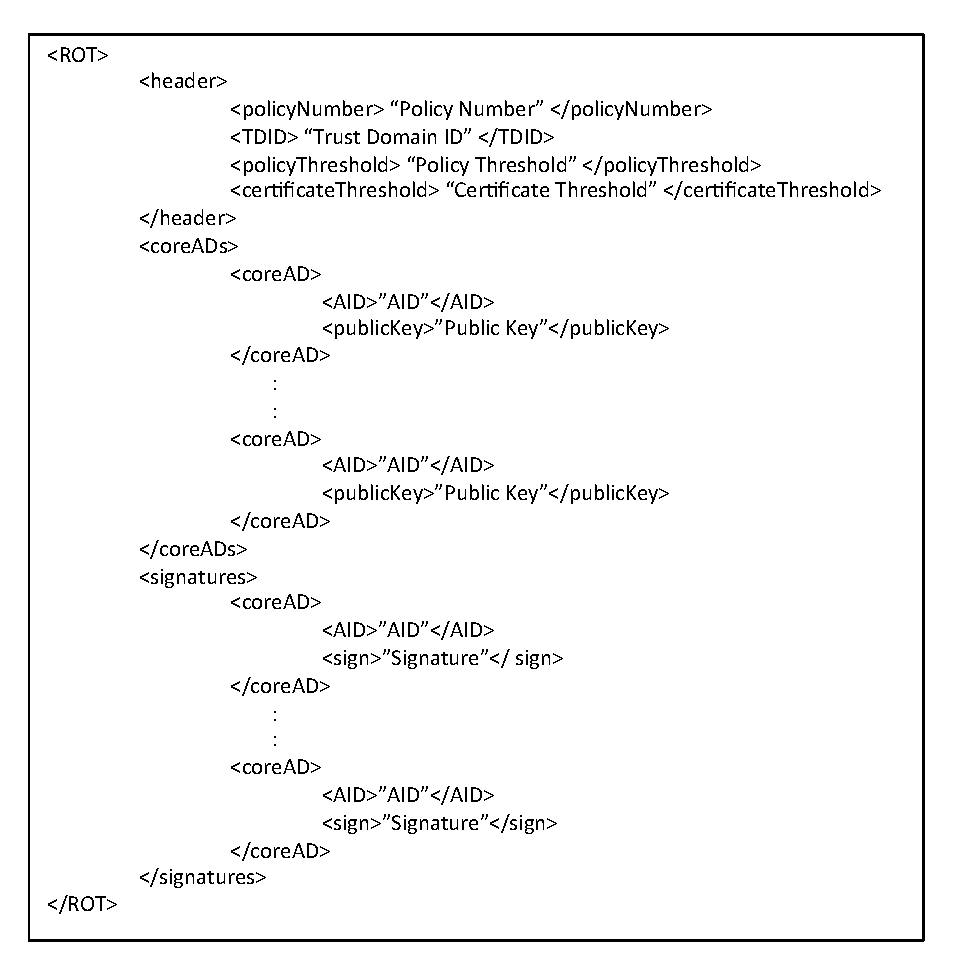
\includegraphics[width=.7\columnwidth]{./fig/rotfile.eps}
%\caption{\RT File Format}\label{fig:rot-file}
\begin{center}
	\fbox{
		\begin{minipage}{\columnwidth}
			\BUseVerbatim[fontsize=\footnotesize]{TopSection}
		\end{minipage}
	}
\end{center}
\caption{Topology File Format}\label{fig:topology-file}
\end{figure}


The \CS distributes server AIDs to border routers so that the border routers forward packets to necessary services. The border routers forward
\begin{itemize}
\item Certificate Request/Response to the \CS
\item PCB to the \BS
\item Path Registration/Resolution to the \PS(s)
\end{itemize}

To forward special packets (i.e., non-data packets listed above) to correct servers, the border routers write the packet's destination AID with the corresponding server's AID. Once the servers process the packets, they remove the destination AID field. This not only make the packet forwarding transparent outside the \AD but also would prevent targeted attacks against those servers.

\section{Bootstrapping}
\noindent {\bf \ISDC \CS: }
The \ISDC is the \RT of an \ISD and the \ISDC \CS has the essential information for establishing \RT. Hence, the \ISDC \CS must be able to start independently. The \ISDC \CS has a local copy of \RT file and all \AD certificates that it has issued (or under itself in \ISDC hierarchy) in its database. The \ISDC \CS communicates with other \ISDC \CSs (if any) in the same \ISD to update the most recent \RT file and necessary (missing) certificates.

\noindent {\bf \AD \CS: } The \CS is the \RT of an \AD as well. The \CS stores the certificates of local entities and the topology file. On its startup, the \CS broadcast server locations inside the \AD and the current OFG key to all border routers. The \CS essentially needs to store the most recent OFG key so that the \CS would not invalidate all opaque fields that are currently being used due to its instantaneous failure. Furthermore, the \CS stores the most recently used (expired) OFG key to help recover the \BS and border routers from their failure. Since an opaque field is valid for 1 day, a border router's Key Table should keep two OFG keys (i.e., the current and previous OFG keys).

\noindent{\bf Assumptions: }
For bootstrapping {em trust}, we make the following assumptions.
\begin{itemize}
\item Trust the \CS(s) in keeping the latest \RT file \chris{How is the \RT kept up to date? Analyzing the communication between BS and CS is needed}
\item \ADs know some public keys of \ISDC \ADs \soobum{necessary? This seems to be a vague assumption} \tenma{Should be. I think it
might be the initial trust. some could changed to ``threshold number''?}
\item \ADs can access the \CS \soobum{This is not an assumption, but a necessary condition for the very initial bootstrapping of SCION}
\end{itemize}

  %\subsection{Root of Trust File} \label{subsec:root-of-trust}
The \RT file contains the list of all \TDCore members, the public keys of these members, and their signatures on the \RT file. The \RT file keeps track of the current policy number and the \ADs that signed the policy. The policy is used as a {\bf \em root of trust} by which all \ADs in the TD establish their trust. The notion of root of trust is crucial in the SCION architecture due to the hierarchical structure of the \TD. As a consequence, the TD membership is strictly limited and agreed by the current members. This is enforced by restricting the update privilege of the \PF. More specifically, the current members of \TDC define the minimum number of \ADs that should provide their signature for updating the \RT file -- defined as {\em Policy Quorum Threshold} ($P_{th}$). Furthermore, the \TDC members define the minimum number of \AD signatures to grant a new \AD's joining to the \TDC and to issue a certificate for the AD. This number, defined as {\em Certificate Quorum Threshold} ($C_{th}$), is also included in the \PF. Hence, an \AD, if it is approved to join a \TDC, would be issued a certificate that is signed by at least $C_{th}$ \TDC \ADs. Figure~\ref{fig:rot-file} shows the contents and the format of the \RT File. 

\begin{figure}[h]
\centering
\includegraphics[width=.7\columnwidth]{./fig/ex_rotfile.eps}
\caption{\RT File Format}\label{fig:rot-file}
\end{figure}

\paragraph{Header}
The header contains the \TDC policy information listed below. 

\begin{enumerate}
\item Trust Domain ID (TD ID or TID) : Globally unique Trust Domain identifier.
\item Policy ID : Current version number of \PF.
\item Policy Quorum Threshold : Minimum number of \TDC \ADs to generate a new \RT file. 
\item Certificate Quorum Threshold : Minimum number of \TDC \ADs to issue a new certificate for an \AD.
\end{enumerate}

\paragraph{\TDC member list}
The \TDC member list contains the information of all \TDC members. Each \AD has the following elements:
\begin{enumerate}
\item \AD ID (AID).
\item \AD's public key.
\end{enumerate}

\paragraph{Signatures}
The signatures element contains the signatures of the \TDC ADs that signed the current \RT file.
\begin{enumerate}
\item AD ID (AID).
\item \AD's signature computed over the header and the \TDC member list.
\end{enumerate}

%\noindent\emph{*Should ask Zhe about Policy in detail. }

  \section{Beacon Server}
The \TDC \BS starts PCB propagation to construct a (half) path from \TDC to \STUB \ADs. The \BS specifies the packet type as PCB in the header (viz., Figure~\ref{fig:hdr-common}), puts its own opaque fields in the packet, and forwards it to customer \ADs. The \BS can specify the next hop \AD (to which it would send PCB) using the egress interface ID since egress interface to \AD mapping is available in the topology file. The ingress routers of an \AD, once they receive a PCB from their provider \AD, forward the PCB to the local \BS; and the local \BS adds its AID and opaque field to the PCB. Every border routers know the \BS location (i.e., address or AID), hence they fill the Destination AID field with the address of the \BS and forward the PCB. The \BS queues all PCBs which arrived within a pre-defined time interval (denoted by $T_Q$), chooses $k$ PCBs per customer \AD, adds its own marking, and propagates them to the chosen \ADs. This PCB propagation ends at \STUB \ADs. We describe how a \BS handles PCBs in detail below.

\begin{figure*}[ht]
\centering
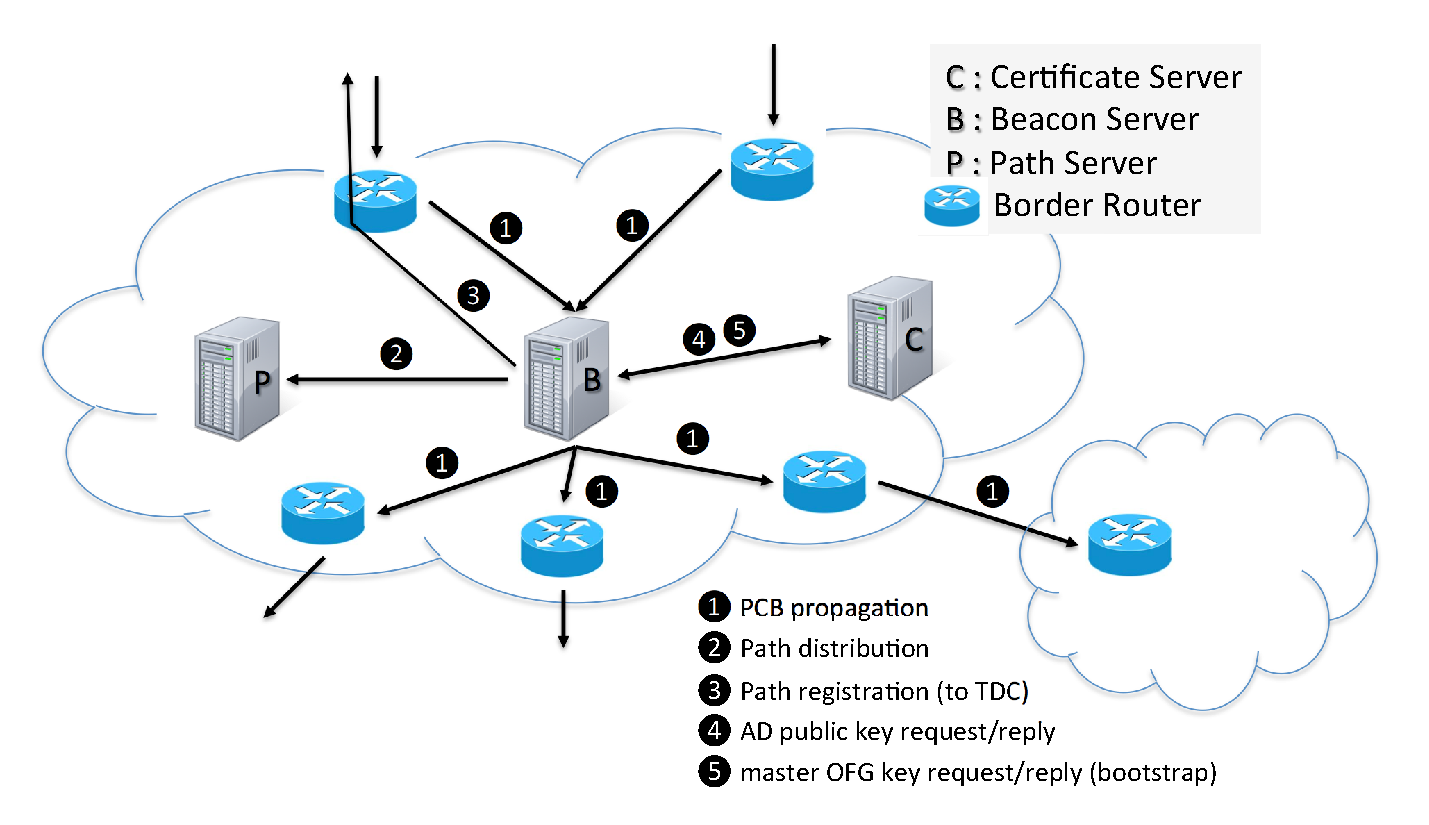
\includegraphics[width=.9\columnwidth]{./fig/bs_message.eps}
\caption{Beacon Server messages.}\label{fig:bs-message}
\end{figure*}

\subsection{Opaque Field Generation}
For path freshness, a \BS generates the opaque field by hashing the current timestamp and expiration time (EXP) with the ingress and egress interfaces. As a result, the opaque fields created with at different timestamps are different even if they have the same ingress-egress interface pair. Furthermore, to limit the path (i.e., opaque field) lifetime, \BSs set the EXP field in the header (viz., Figure~\ref{fig:hdr-common}) to one of four types (i.e., 6, 12, 18, 24 hours) based on their local policy. Since all border routers know the current and previous OFG keys, they can compute the opaque field for a specific timestamp and hence verify the opaque field carried in a data packet (that was originally generated by the \BS). We note that every data packet carries the timestamp and expiration in its header. %Once a border router receives a OFG key, the router stores the key in its {\bf Key Table} so as to reuse that key (without hash computation) for verifying other packets carrying the same timestamp.

{\bf Key management:} Key revocation and recovery after failures or compromise. \soobum{Key recovery seems not an issue, yet revocation needs to be preceded by identification of key compromise}

\subsection{PCB Selection/Propagation}~\label{subsec:pcb_selection}
The \BS queues PCBs for a predefined PCB propagation period (e.g., 10
seconds), and selects $k$ PCBs to propagate to customer \ADs, each of
which may have a different set of selection policies. We consider two
classes of policies: (1) exclusion and (2) prioritization. Exclusion
policies specify paths that should be avoid, and prioritization
policies specify the preference between paths.

The current implementation supports four exclusion policies that we
believe are commonly used:
\begin{itemize}
\item {\bf Maximum age ($A_{max}$, in seconds)}: The age of a PCB is
  defined as the length of time that the PCB has existed. This policy
  excludes paths with age above $A_{max}$.
\item {\bf Maximum path length ($L_{max}$, in hops)}: This policy
  excludes paths above $L_{max}$ AD-level hops.
\item {\bf Minimum elapsed time since last propagation ($E_{min}$, in
  seconds)}: While we flexibly allow re-propagation of the same PCB
  (for reasons like improving fault tolerance), we also would like to
  maintain a good level of path diversity by not propagating the same
  PCB over and over again in a short period of time. Hence, this
  policy excludes paths that have been propagated in last $E_{min}$
  time.
\item {\bf Unwanted ADs:} This policy allows exclusion of paths
  containing certain ADs. For example, the administrator may want to
  avoid going through ADs that are identified to be malicious or
  provide low quality services.
\end{itemize}

The rest of the PCBs are prioritized based on their {\bf Path
  Fidelity}, a metric defined in terms of age, path length, and path
freshness. We would like to incorporate other parameters such as
local desirability, available bandwidth, and disjointness in the
future. 


%% PCB selection is determined using {\bf Path Fidelity} defined in terms
%% of local desirability, path length, path freshness, and available
%% bandwidth.

\begin{itemize}
\item {\bf Age ($A_p$):} As defined earlier, the age of a PCB is the
  length of time that the PCB has existed.
\item {\bf Path length ($L_p$):} \AD-level path length to \TDC. The
  path length is the most {\em stable} and {\em reliable} estimate for
  path quality.
\item {\bf Path freshness ($E_p$):} time elapsed since a path's last
  propagation. Non-propagated paths for a while would have higher
  freshness and hence have chance to be selected; e.g., a maximally
  disjoint path from previous propagations would be selected with
  higher probability.
\item {\bf Local desirability ($D_p$):} a value ranging from 0 to 1,
  where 1 indicates the highest desirability. An \AD decides a path's
  local desirability based on the contracts with provider and customer
  \ADs or to optimize its local network resource (e.g., local traffic
  engineering).
\item {\bf Available bandwidth ($B_p$):} available bandwidth would be
  the most accurate measure of path quality if long-term (e.g., hours
  rather than seconds), static bandwidth allocation can be made.
\item {\bf Path disjointness:} how much the current path differs from
  all previous selections. We can quantify the path disjointness by
  the number of new ADs the current PCB covers.
\end{itemize}

In the current implementation, the prioritization policies specify the
weights ($w_1$, $w_2$, and $w_3$) of each term in computing path
fidelity:
\[
F_p = 1 - (w_1 \cdot \frac{A_p}{A_{max}} + w_2 \cdot \frac{L_p}{L_{max}} + w_3 \cdot \frac{E_{min}}{E_{p}})
\]
Note that when $w_1 + w_2 + w_3 = 1$, $F_p$ is between 0 and 1.

%% The path fidelity, denoted by $F_p$, is defined in terms of the above metrics.
%% \[
%% F_p = w_1 \cdot D_p + w_2 \cdot \frac{L_{MIN}}{L_p} + w_3 \cdot \frac{E_p}{E_{MAX}} + w_4 \cdot \frac{B_p}{B_{MAX}}
%% \]
%% where $L_{MIN}$, $E_{MAX}$, and $B_{MAX}$ are the minimum path length,
%% maximum freshness, and the maximum available bandwidth
%% respectively. 

The \BS distinguish a path by a series of tuples, namely AID, ingress
interface and egress interface, marked by each \AD. Newly arrived PCBs
are added to a {\em beacon table}, and the \BS maintains the size of
the beacon table by removing oldest PCBs (PCBs with smallest
timestamps).  \note{HC: the current implementation doesn't seem to
  detect duplications...}  Periodically, the \BS initiates the path
selection process as follows. For each customer \AD, the \BS
prioritizes and filters PCBs in the beacon table according to this
\AD's policies, propagates to the \AD $k$ PCBs with the highest
priority, and keeps track of what PCBs have been propagated. The \BS
can also select paths in a probabilistic fashion: instead of selecting
the top-$k$ paths, the \BS scans paths from the highest priority to
the lowest, and selects each path with a certain probability until $k$
paths are selected.


%% When a new PCB arrives, the \BS queues the PCB in its local buffer
%% after checking duplicate and assigning a local timestamp (as
%% opposed to the global timestamp marked by \TDC) to the PCB. If the
%% \BS cannot find a duplicate path in its PCB queue, it assigns a
%% current local timestamp to the PCB, which would be used for
%% computing path freshness. If the \BS find a duplicate, it copies
%% the old (duplicate) PCB's local timestamp to the new PCB and
%% replaces the old PCB with the new one. That is, for each path, the
%% \BS only keeps the most recently arrived PCB while keeping track of
%% the age of the path (i.e., how long the path was kept in the queue
%% without being propagated). The \BS controls the diversity of
%% propagated paths by adjusting $A_{max}$: e.g., a lower $E_{MAX}$
%% would increase the path diversity.  The \BS selects a PCB from its
%% PCB queue with a probability proportional to the path fidelity
%% computed by the above equation.

%\soobum{More details on path selection algorithm need to be described and analyzed}


\subsection{Path Registration/Distribution}
An \AD's \BS selects $k$ paths from all received PCBs in order to provide remote source \ADs with down-paths and help those \ADs to establish end-to-end paths. To this end, the \BS registers the selected paths to the \TDC \PS. The \BS does not need to register $k$ paths at a time, yet can register paths whenever it wants to do. However, the number of total registered paths at the \TDC \PS cannot exceed $k$. The path registration request should be signed by the requesting \AD to prevent any forgery by malicious \ADs. The \TDC \PS, on receiving a path registration request, verifies the signature and registers the path as: if the \PS has less than $k$ registered paths for the \AD, it registers the path; otherwise the \PS replaces the oldest path (that has the smallest timestamp) with the new one. The \PS limits the number of \AD's path registrations to prevent malicious \ADs from overloading the \TDC \PS and from exploiting too many paths (for attack purposes).

The \BS informs $k$ registered paths to local \PS(s) so that these paths can be used as up-paths to \TDC. Note that the local \PS provides $k$ up-paths to endhosts. Furthermore, the \BS provides some of non-registered paths to the local \PS. These non-registered paths can be used as up-paths as well, yet the packets forwarded along the non-registered paths have low priority than those of registered paths in the presence of congestion. \soobum{need to refer to the SCION DDoS to explain packet priorities}

\begin{comment}
\subsection{Key Table Management}~\label{subsec:key-table-management}
The \BS generates an OFG key by hashing the current timestamp in the PCB (marked by the \TDC \BS) and its own expiration time with the master OFG key; i.e., $K_i(t)$ = $\textrm{H}_{K_i^{master}}(\textrm{timestamp} || \textrm{EXP})$. Since border routers know $K_i^{master}$, they can verify the opaque field carried in a data packet after computing $K_i(t)$. However, the border routers, instead of computing $K_i(t)$ for every packets, keep $K_i(t)$ in their Key Table for up to its expiration time in order to reduce computational overhead. With this, the router would lookup the key table first and if the table contains a stale (i.e., expired) key for the corresponding time, the router compute and store the OFG key. For example, if a PCB is generated in every 1 minute, the routers need to keep at most 1440 $\times$ 4 = 5760 keys, which only requires a small amount of memory (less than 100KB for 128 bit keys) while enabling fast key retrieval from the table (a router determines a key location in the memory using the timestamp and expiration time). \ADs synchronize timestamp using a time server or a satellite time. Time synchronization can be made with low precision if \PSs and border routers allow a sufficient grace period (e.g., several minutes) after a path expires.\soobum{Need to elaborate the time synchronization; e.g., when it's required} 
\end{comment}

\subsection{Bootstrapping}
The \BS has to be prepared with the following information for PCB propagation.
Specifically, the \BS retrieves 
\begin{itemize}
\item the OFG key from the \CS for Opaque Field generation 
\item \AD public keys for PCB verification
\item the topology file from the \CS for PCB propagation
\end{itemize}
The \CS handles all intra- and inter-AD certificate requests and stores the results for all entities within an \AD. Hence, the \BS contacts the \CS to get necessary \AD public keys for signature verification. To reduce the communication overhead during bootstrapping, the \BS starts with local copies of the above data and update them later if necessary. We note that the topology file and \AD public keys not frequently changed (i.e., static), hence they can be stored at the \BS. The \BS reads inter-\AD connectivity information from the topology file and decides how to propagate PCBs. Specifically, the \BS propagates PCBs to the interfaces that connect to customer \ADs (this information is contained in the topology file). Initially, the \BS sets the status of all interfaces registered in the topology file to {\em active} in its local database; yet the \BS changes the status to {\em inactive} for any interface to which propagating a PCB failed. \soobum{A control message protocol (like ICMP) and error messages (or codes) need to be defined.}

\begin{comment}
PCB Propagation
Maintain most recent (Timestamp, Opaque Field Generation Key) acquired 
from Certificate Server (CS)
	Request the pair to CS if it does not have (e.g., due to reboot)
	How often should the OFG Key renew?
Maintain (AID, Public-Key) for PCB signature verification 
	Request the pair to CS if it does not have (first seen AID)
Start Queueing PCBs if a new timestamp arrives – use per child AD queue / verify sign. on arrival
Stop Queueing PCBs if current_time – start_time(of current timestamp) > MAX_PROP_DELAY
Pick k PCBs per child AD based on the preset rules; 
	0. local policy (traffic engineering)
	1. shortest path length
	2. maximally disjoint from previous n propagation
	3. ?
Mark Opaque Field with the present OFG key; H(master OFG key||timestamp)
Propagate k PCBs to children and purge Queue
Add the present OFG key to Key Table (index, the present OFG key)
Multicast all (or selected) Paths to local Path Servers after removing all signatures and adding its own signature (use for best effort paths)
\end{comment}

  \section{Path Server}
The \TDC \PS maintains a path database that contains all $k$ paths registered by \STUB \ADs, and provide down-path resolution service to support \AD-level end-to-end path establishment.

\begin{figure*}[ht]
\centering
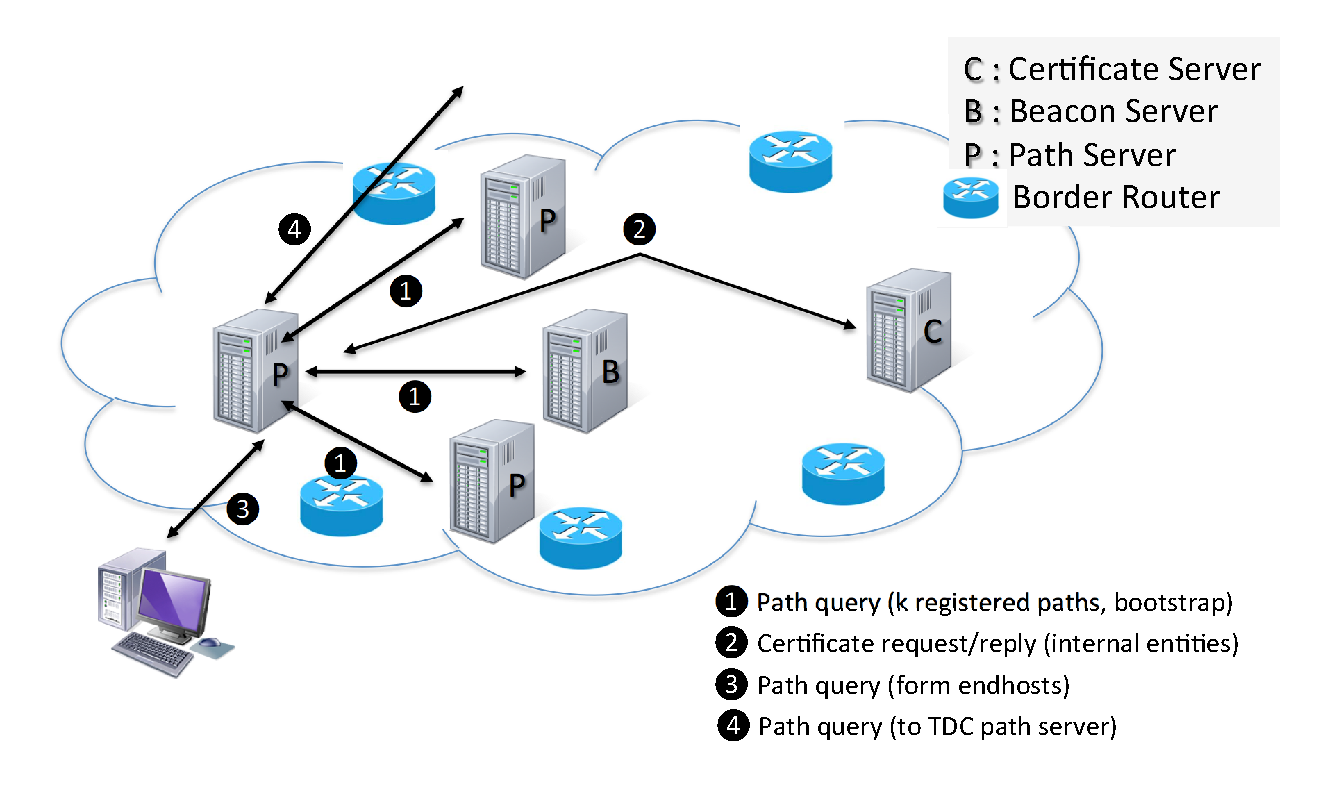
\includegraphics[width=.9\columnwidth]{./fig/ps_message.eps}
\caption{Path Server messages.}\label{fig:ps-message}
\end{figure*}

\subsection{Path Registration}
An \STUB \AD's path registration request includes the following information.
\begin{itemize}
\item {CTime: } Current time 
\item {AID: } ID of the requesting \AD %\newline
\item {Type: } [Public/Private], [Internal/External] %\newline
\item {Timestamp: } \TDC's timestamp that shows the PCB initiation time 
%\item {Expiration Time: } Lifetime of the path. (Currently, we define 4 lifetimes: 6 hours, 12 hours, 18 hours, and 24 hours; viz., Figure~\ref{fig:hdr-common})
\item {Hops: } The number of \ADs (i.e., \AD hops) from \TDC to the \STUB \AD
\item {PCB Header: } A series of AIDs and corresponding Opaque Fields (viz., Figure~\ref{fig:hdr-beacon}) %\newline
\item {Signature: } The requesting \AD's signature computed over the registration request information %\newline
\end{itemize}

\noindent The current time (CTime) is added to prevent replay attacks. The {\em Type} field determines the scope of path disclosure and is defined as follows. %\newline
\begin{itemize}
\item {Public (TYPE\_PUB): } A public path is used by all \ADs. %\newline
\item {Private (TYPE\_PRI): } A private path is encrypted with a secret key. This path can be used by the \ADs that know the secret key and hence decrypt the path information. %\newline
\item {Internal (TYPE\_INT): } An internal path is disclosed to the \ADs inside the TD %\newline
\item {External (TYPE\_EXT): } An external path is disclosed to all \ADs outside the TD %\newline
\end{itemize}

The \TDC path server, on receiving an \AD's path registration request, verifies the signature in the request, and if the signature is correct, it replaces the \AD's oldest entry with the new path. If the path registration fails, the path server returns an error code. Possible error code includes:

\begin{itemize}
\item Unidentified \AD (including missing \AD certificate)
\item Signature verification failure
\item Maximum number of updates exceeded
\end{itemize}

Note that path registration is made to the path server in the \TDC.

\subsection{Path Resolution} 
\STUB \ADs use the registered $k$ paths to the \TDC for up-paths and down-paths ($k$ up-paths and $k$ down-paths can be different). A source \AD, in order to know how to reach the destination \AD (we assume that the sender (host) knows the AID of the destination \AD that hosts the receiver (host), using a DNS service), sends a path query to the \TDC path server. The \TDC \PS's response includes $k$ down-paths to the destination \AD, where each down-path is a series of ADs and their Opaque Fields. Then, the source \AD selects a down-path and constructs an end-to-end path by composing one of its up-path and the selected down-path.

To perform the above path resolution, the \TDC \PS and local \PS should provide the following functions.

\noindent {\bf \TDC \PS: } The \TDC \PS, on receiving a path query, determines which paths to return using the AID and Type in the packet. If the server has the corresponding paths to the query, it sends paths to the requesting \AD. The query response is signed by the \TDC \PS. \soobum{needs discussion. Signature on the query response is necessary for security, yet would introduce overhead to the \PS.} The \TDC would have multiple \PSs for load balancing and replication. A Distributed Hash Table (DHT) would be a good practical candidate for distributed \PS implementation. \soobum{do we need to elaborate this?}


\noindent {\bf Local \AD \PS: } Local \PSs resolve both up-paths and down-paths for endhosts. For up-path resolution, a local \PS keeps the list of paths offered by the \BS in the same \AD. The \BS, whenever it receives a new path (i.e., PCB) to \TDC,  multicasts the path to all \PSs inside the \AD. That, a local \PS is a passive server. However, the \PS, on its first wake-up, pulls the registered up-paths to \TDC from other \PSs within the \AD; or the server pulls those paths from \TDC (note that un-registered, low-priority up-paths are multicast to \PSs continuously). An endhost set AID to TDC for an up-path query. For down-path service, a local \PS send a path query to the \TDC on behalf of an endhost and forward the response from the \TDC to the endhost. Furthermore, the local \PS stores the query response in its local cache to promptly handle the same path request from other endhosts. Down-path caching help reduce path resolution latency and prevent frequent path requests to \TDC that would overload the \TDC \PSs.



\subsection{Path Database}
For path resolution services, \PSs maintains the following database.

\noindent {\bf \TDC \PS: } Down-paths to \STUB \ADs inside the \TD. \newline
A record of an \STUB \AD consists of the path registration information shown above.

\noindent {\bf Local \PS: } Up-paths to \TDC and down-paths to remote \STUB \ADs.
A record of an up-path has the same format as that of down-paths, yet it ends with a \TDC \AD instead of an \STUB \AD. The local \PS cache has the same data structure as that of the \TDC \PS.

\subsection{Bootstrapping}
The \TDC \PS are assumed to be highly replicated and synchronized. Hence, when a \PS starts and finds any other \PSs in the topology file (that is kept locally or retrieved from the \CS), the \PS synchronizes its database with those of other \PSs. Bootstrapping procedure may differ how \PS database is implemented (e.g., RDB, DHT). Currently, the \PS stores the snapshot of path database as a file periodically (in every 10 minutes). Local \PSs works similarly, yet they only synchronize up-paths (or at least registered $k$ up-paths, which can be retrieved from the \BS if the \AD has a single \PS) to \TDC. Cached down-paths to remote \ADs are not required to be synchronized. 




  \section{Border Router}
A SCION border router forward a packet either to an internal server or to an egress interface based on the packet type. 
\subsection{Data Packet Forwarding}
A SCION data packet is the packet that does not go through any server (i.e., \CS, \BS, \PS) and carries a series of opaque fields from a source to a destination (i.e., an end-to-end communication packet). When an ingress router of an \AD receives a SCION data packet, the router (1) looks at the current hop (to find out which opaque field it has to verify), (2) verifies the opaque field, (3) increases the Hops field by one (viz., Section~\ref{subsec:common-header}) if the verification passes, and (4) forwards the packet to the egress interface specified in the opaque field. For opaque field verification, the router computes a key that corresponds to the timestamp and expiration time in the packet. As described in Section~\ref{subsec:key-table-management}, each border router first refers its Key Table to get the key and then if the table does not hold a valid key record (i.e., either does not have a record or has a expired key), the router computes the corresponding key and stores it to the table. 

A series of opaque fields represent an interface-level \AD path from the \TDC to a \STUB \AD. Since the ingress interface of an opaque field is determined by the PCB propagation direction (i.e., an interface to a provider is always an ingress interface), the interface needs to be switched 

\subsection{Control Packet Forwarding}
A SCION control packet is the packet that needs to be delivered to any one of the servers. For example, a PCB needs to be delivered to the \BS; a certificate request to the \CS, and a path registration/resolution to the \PS. All control packets do not include the destination AID field in the SCION header, yet are distinguished as such by the packet type. Border routers, when they receive a control packet, write the destination AID with that of the corresponding server using the up-to-date server locations advertised by the \CS. Intra-\AD routing/forwarding protocol deliver control packets to the corresponding servers using the destination AID. 

{\bf PCB propagation: } The ingress (border) router of an \AD, when it receives a PCB from its parent \AD, writes the Current IF field of the header (viz., Figure~\ref{fig:hdr-common}) with the interface ID at which at PCB arrive, in order to help the \BS to generate a opaque field (note that ingress interface ID is necessary for MAC generation).
 
\subsection{Bootstrapping}
A border router, on its startup, register itself to the \BS so as to receive PCBs from the \BS. This registration would be invalidated if the \BS receives an PCB propagation error message. \soobum{We have to define error messages for troubleshooting and maintenance; e.g., PCB propagation error.} The router retrieves the current and prior master OFG keys from the \CS. Since an opaque field is valid for a day, the Key Table entries are generated either by the current or by the previous master OFG key. Hence, the router is able to construct its Key Table with those two master OFG keys. And, the border router should get the server locations from either any neighboring router or directly from the \CS. The border router specifies its request in the SCION header, and an internal router of the \AD responds this request or forwards it to the \CS. We note that the master OFG response is encrypted includes the MAC generated by the \CS; and the server location response includes the \CS's signature.

  \chapter{Packet Formats}~\label{sec:packet-format}
In this section, we describe the SCION header format. The SCION header consists of two parts: the common header and the protocol header. 
The protocol header is defined differently by the contents of a packet. Currently, we have two protocol headers: one for PCBs, and the other one for all other data packets.


\section{Common Header}~\label{subsec:common-header}
All SCION packets have the common header. The common header contains the most basic packet information that is necessary for all SCION packets. The Figure~\ref{fig:hdr-common} shows the common header format.

\begin{figure}[ht]
\centering
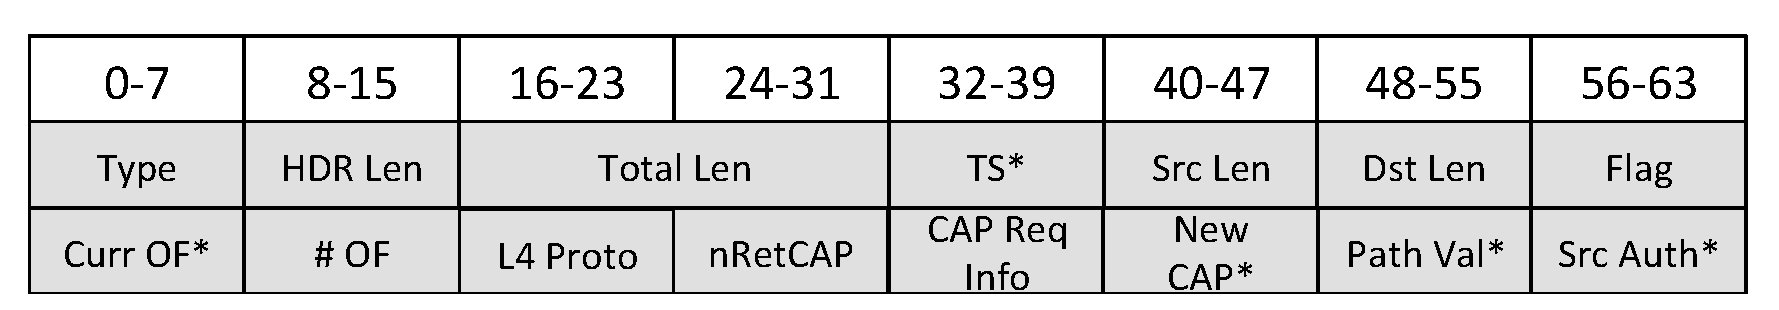
\includegraphics[width=.9\columnwidth]{./fig/nhdr_common.eps}
\caption{Common Header.}\label{fig:hdr-common}
\end{figure}

\begin{itemize}
\item{Type: } BEACON, DATA, CERT\_REQ, CERT\_REP, PATH\_REG, PATH\_REQ, PATH\_REP
\item{HDR Len: } Common header length
\item{Total Len: } Total packet length (including header)
\item{TS*: } Pointer (or offset in Bytes from the beginning of payload) to the current timestamp. Note: up-path and down-path have different timestamps marked by different TDC ADs. The first router on the down-path updates this pointer with the offset to the special opaque field that contains down-path timestamp.
\item{Src Len: } The length of source address, e.g., 4B for IPv4 and 16B for IPv6. Any (new) address can be supported. This field can be zero for special control-plane messages (e.g., BEACON message does not require the source address). 
\item{Dst Len: } The length of destination address. This field can be updated by border routers if they put an internal server's address. For example, if a border router receives a BEACON message, the router sets the Beacon Server's address to the destination address field and its size to the Dst Len field. 
\item{Flag: } Path status information. Each bit (from the MSB) has the following meanings -- (0) up/down path, (1) overuse, (2) congestion.\footnote{overuse and congestion bits are used in STRIDE (i.e., SCION DDoS extension).} 
\item{Current OF*: } The pointer to the current opaque field. An ingress router (of an AD) processes a data packet with the opaque field specified in this pointer.
\item{\# OF: } number of opaque fields in the current marking. This would be used for an offset to the capability field.
\item{L4 Proto: }  Upper-layer transport protocol, e.g., TCP, UDP
\item{nRetCap: } The size of the return capability (which consists of a series of router capabilities). 
\item{Cap Req Info: } Capability request information
\item{New CAP*: } Offset to the new capabilities. If the packet type is capability request (CAP\_REQ) or renewal (CAP\_RENEW), routers on the forwarding path write new capabilities in this field.
\item{Path Val*: } Pointer to the {\em path validation} information (variable size)
\item{Source Auth*: } Pointer to the {\em source authorization} information (variable size)
\end{itemize}


\section{Beacon Header}
An \AD's beacon server, when it receives a PCB from its provider \AD, adds its own marking and signature to the PCB; and forwards the PCB to its customer \AD. Hence, a PCB eventually constructs a path from \ISDC to an \STUB \AD. Figure~\ref{fig:hdr-beacon} shows the beacon header format.

\begin{figure}[ht]
\centering
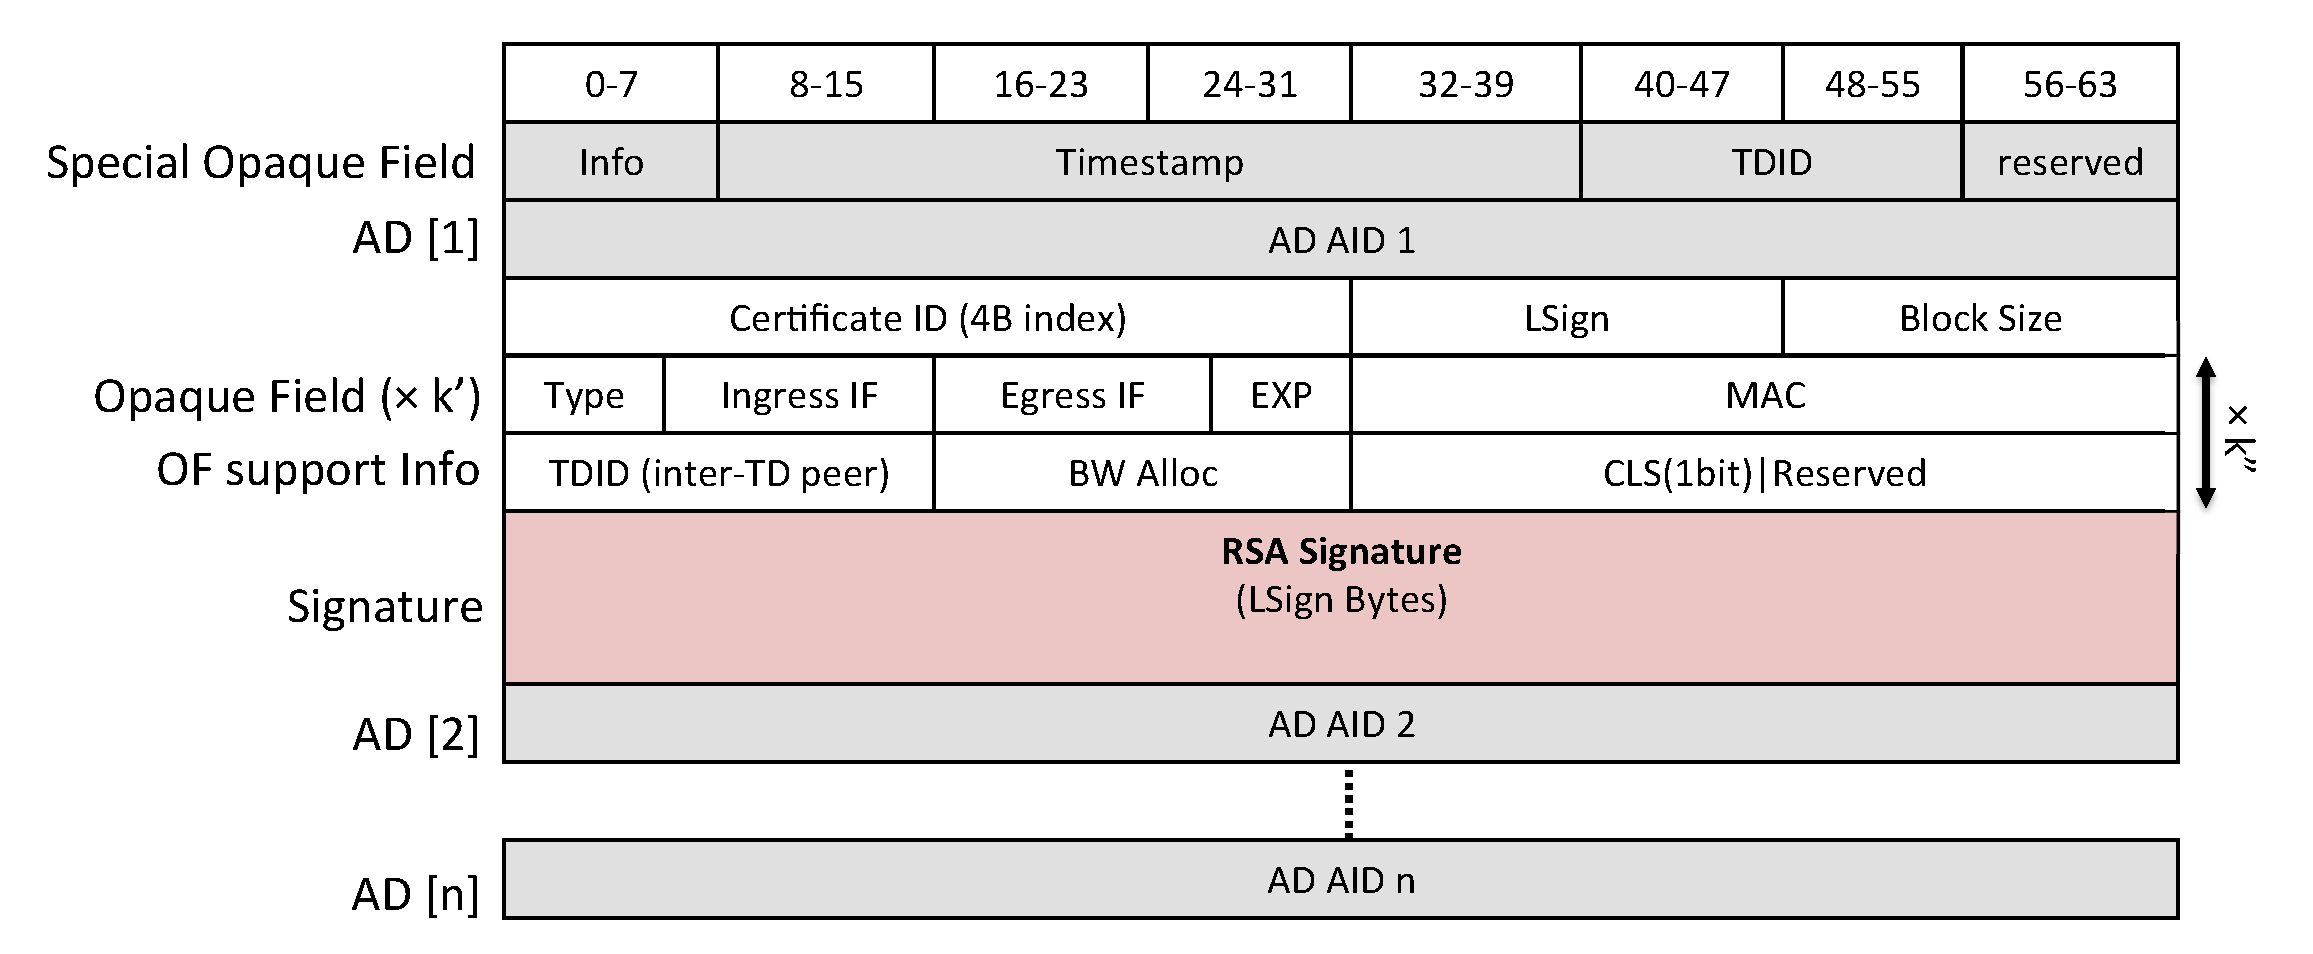
\includegraphics[width=.9\columnwidth]{./fig/nhdr_pcb.eps}
\caption{Beacon Header.}\label{fig:hdr-beacon}
\end{figure}

\begin{itemize}
\item{Info: }This field is used for data packets. To make the opaque field format consistent (i.e., 8B aligned) over all opaque fields.
\item{Timestamp: }PCB's timestamp marked by its initiator (i.e., \ISDC \BS).
\item{AD AID: } authenticated ID of an \AD (this can be the hash of an AD's public key).
\item{Certificate ID: } ID of the certificate (i.e., the signed public key) used for RSA signature generation. Change of this value signals the change of the current AD's certificate and would have BSs retrieve the new certificate from the \CS.
\item{LSign: } signature length; e.g., 1024 bits, 2048 bits
\item{Block Size: } the total size of block marked by an \AD (in bytes), which determines the offset from which a new AD marking starts
\item{Type (4 bits): } This field indicates whether the current opaque field continues in the next opaque field or not. Zero in the MSB indicates the current opaque field is the end of the opaque field. If an AD needs more than 8B for its marking, it set the MSB and add more information to the next 8B, thereby the AD can use several 8B-aligned opaque field blocks. 
\item{Ingress IF (13 bits): } ingress interface id (internal use)
\item{Egress IF (13 bits): } egress interface id (internal use), or egress interface of peer (for a peering link, the egress interface to the customer AD is same as that of the first opaque field because a PCB is send to a single egress interface)
\item{EXP (2 bits): } lifetime of the path; current assignment: 00 - 6HR, 01 - 12HR, 10 - 18HR, 11 - 24HR
\item{MAC: } Massage Authentication Code, MAC(i) = $AES-CBC-MAC_{K_i}$(Ingress IF$||$Egress IF$||$OF(i-1)$||$ AD$_{next}$) \newline
	$K_i$ – MAC generation key of AD[i], AD$_{next}$ is the AD[i]'s customer to which the PCB is forwarded. MAC chaining would prevent (malicious) splicing of opaque fields.
\item{ISD ID: } Trusted Domain ID, which is used only for Inter-ISD peering link
\item{Signature: } RSA signature signed by AD[i]
\end{itemize}

An \AD can add all its peering links to a PCB. The \BS, when it constructs an opaque field for a peering link, fills the Egress IF field with that of the peer so that the \STUB \AD can find an interface-level shortcut. However, the MAC of a peering link should not be computed with the Egress IF field but be computed with the Egress IF to which a PCB propagates. Since the opaque field of a non-peering link (i.e., the opaque field for the path from \ISDC) has the actual egress interface ID, the \BS uses this egress IF in generating the MAC of a peering link. An \STUB \AD, when it constructs a path using a peering link, the \AD writes the egress IF of the opaque field of the peering link with the one used for the MAC generation. And, the \BS does not incorporate the previous \AD's opaque field (i.e., OF(i-1)) in generating the MAC of a peering link since OF(i-1) would not be present at the SCION header when a \STUB \AD constructs a path (i.e., a series of opaque field) using a peering link. An \AD generates its signature by (1) computing a MAC using its markings (including those for the peering links) and the next-hop AD's AID as inputs and (2) then encrypting the message digest with its RSA private key.

\section{Data Header}\label{subsec:data-header}
A data packet, in addition to the common header, carries a series of Opaque Fields that represent an end-to-end path collectively.

\begin{figure}[ht]
\centering
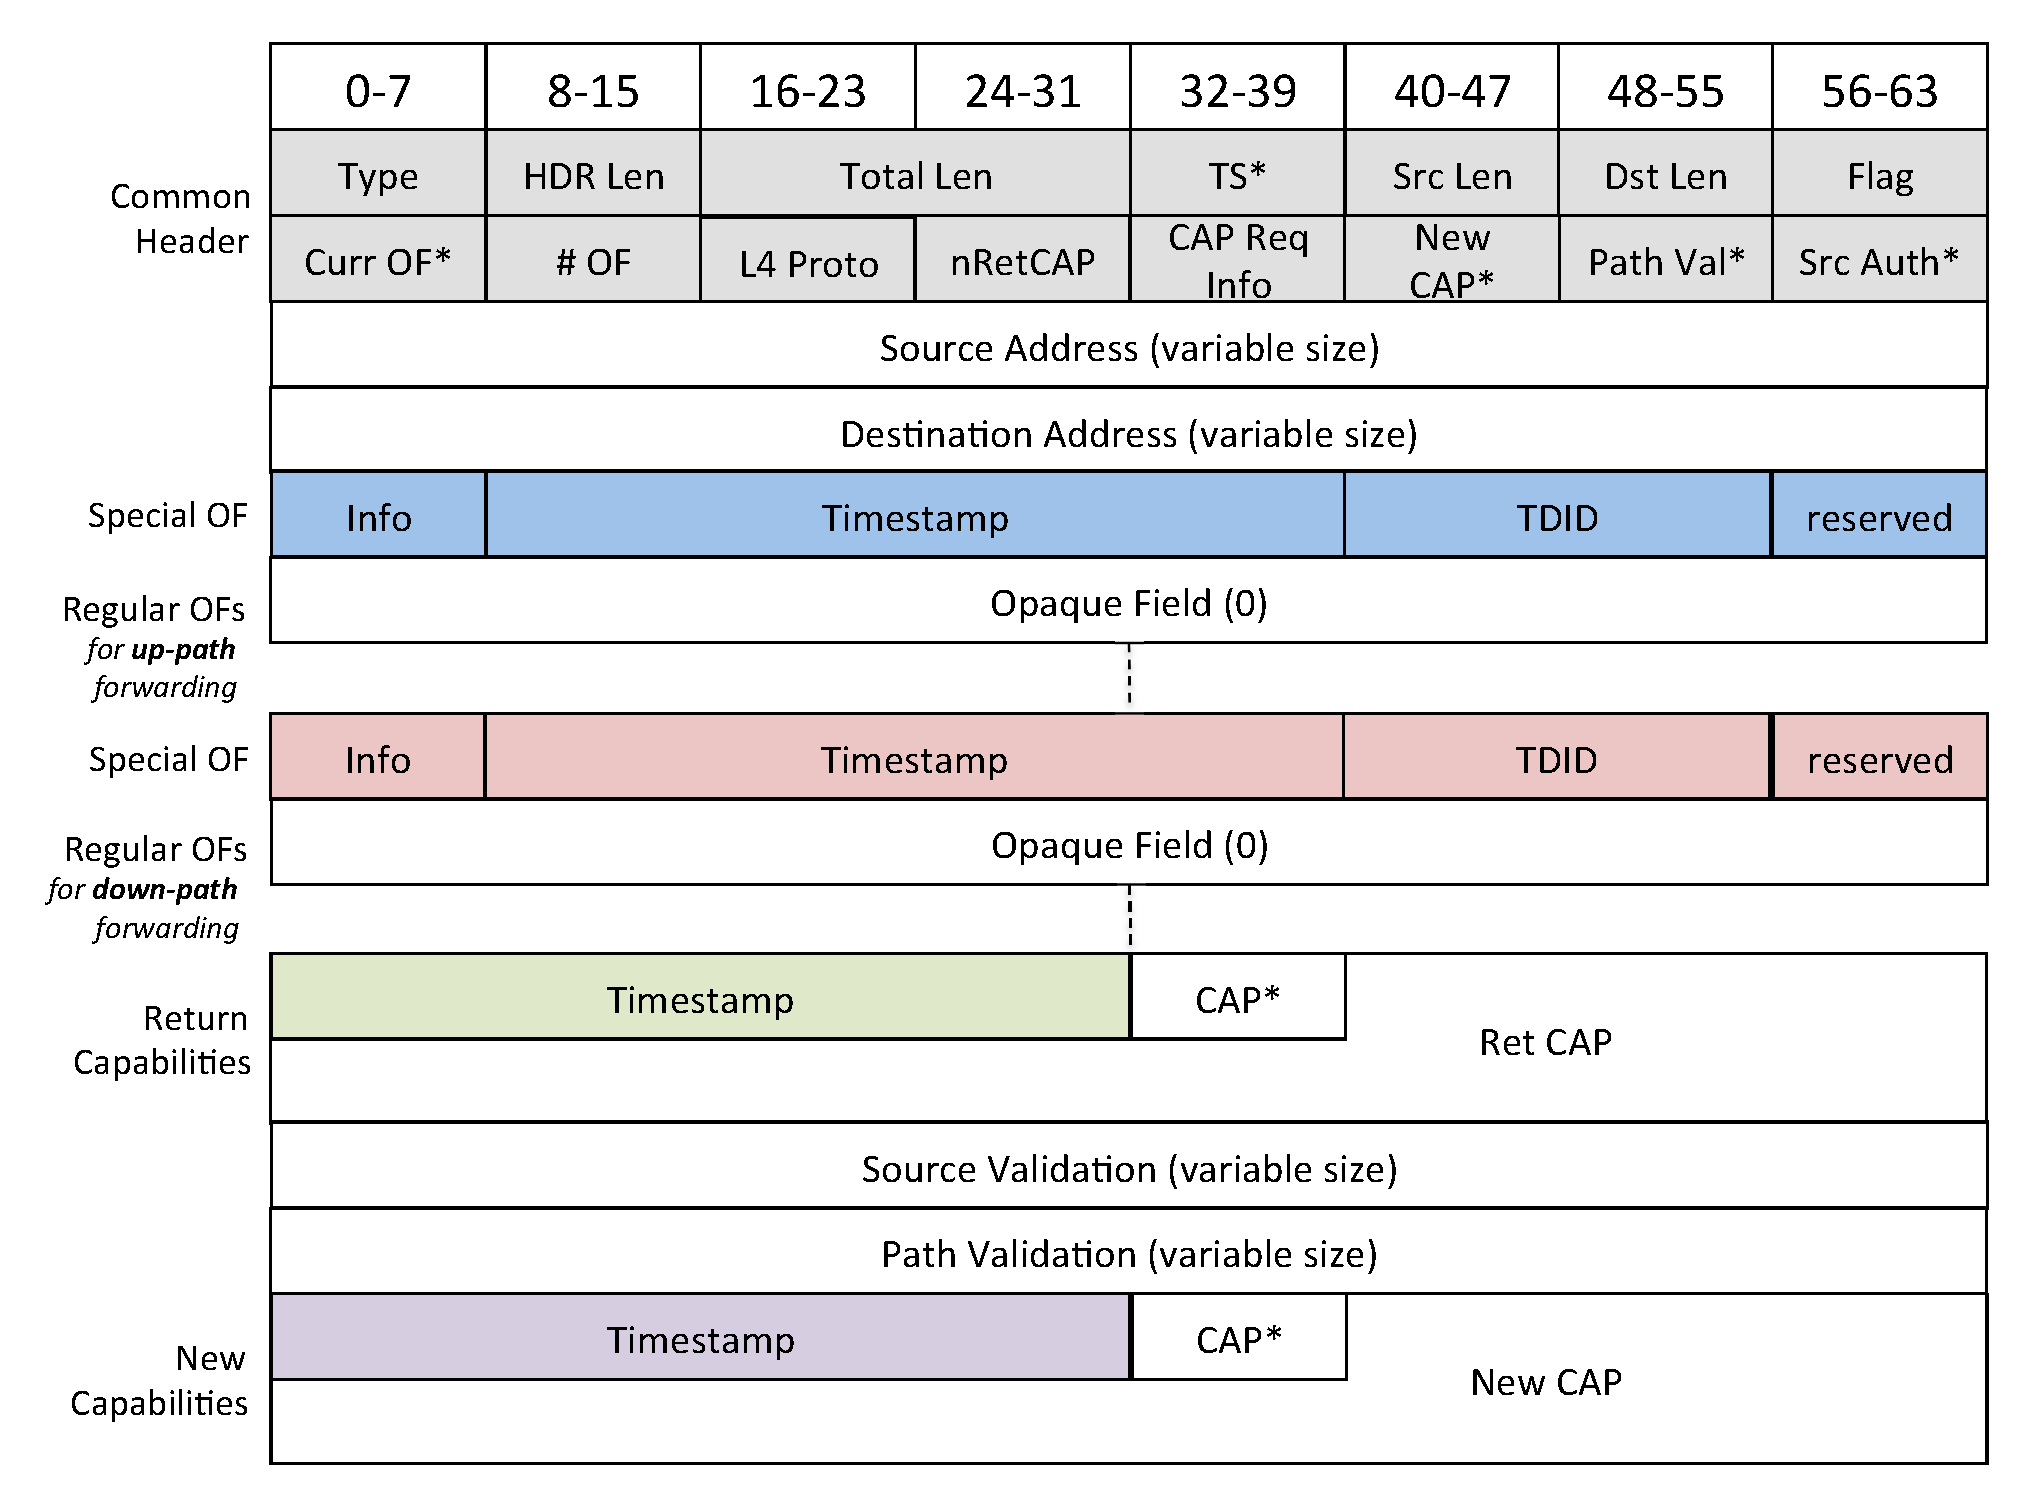
\includegraphics[width=.9\columnwidth]{./fig/nhdr_data.eps}
\caption{Data Header.}\label{fig:hdr-data}
\end{figure}

\begin{itemize}
\item{Special Opaque Field: }This opaque field contains the timestamp that \ISDC \AD marked into the PCB and the isolation domain ID the \AD belongs to. Since this timestamp is valid for a half-path (i.e., from \ISDC to an \STUB \AD), at least two timesstamps (one for up-path and one for down-path) are present in a packet. If a packet traverses multiple \ISDs, it should contain as many timestamps as the number of \ISDs. Info field contains the information regarding a series of opaque fields that use the same timestamp and informs ADs on the path of how to handle opaque fields. Note: Special opaque field processing is required if an \AD is at the crossover point (i.e., at the point where up-path to down-path transition occurs). Info field has the following meanings.
	\begin{itemize}
	\item{0xxxxxxx}: Normal opaque field. A router processes a single opaque field.
	\item{1xxxxxxx}: Special opaque field. The next byte starts with a 4B timestamp. The ingress router has to update the OF* in the common header with the current (special) opaque field.
	\item{10xxxxxx}: Normal ISD core path (i.e., source \AD $\rightarrow$ TDC $\rightarrow$ destination \AD).
	\item{11xxxxxx}: Shortcut path.
	\item{110xxxxx}: Normal shortcut through a common AD of up- and down-path.
	\item{111xxxxx}: Normal shortcut (in-path, viz., example in Figure~\ref{})
	\item{1111xxxx}: Shortcut through a peering link between ASs.
	\item{11110xxx}: Intra-ISD peering link
	\item{11111xxx}: Inter-ISD peering link
	\end{itemize}
Reserved field can be used to specify the size of each opaque field block (i.e., up-path block, down-path block, TDC path block). Using this block size, ADs can quickly identify {\em ISD path} if necessary.
\item{Regular Opaque Field: }Regular opaque fields are used for each router in forwarding packets. A router verifies a packet's MAC with the embedded ingress and egress interface information and if the MAC is correct, the router forwards the packet to the egress interface.
	\begin{itemize}
	\item{Type (4 bits): } Opaque field type. 
		\begin{itemize}
		\item{00xx}: End (indicate the current opaque field ends here). Note: an AD can write multiple blocks of opaque field.
		\item{01xx}: Continue (indicates the current opaque fields continues in the next 8B).
		\item{001x}: Crossover point (inform a router to handle more opaque field based on the crossover type). Crossover point must be specified in all packets.
		\end{itemize}
	\item{Ingress IF (13 bits): } ingress interface id (internal use)
	\item{Egress IF (13 bits): } egress interface id (internal use)
	\item{EXP (2 bits): } Expiration time of the Opaque Field (00: 6 hours, 01: 12 hours, 11: 18 hours, 11: 24 hours)
	\item{MAC (32 bits): } Massage Authentication Code, MAC(i) = $AES-CBC-MAC_{K_i}$(Ingress IF$||$Egress IF$||$OF(i-1)$||$AIDi+1)\newline
		$K_i$ – MAC generation key of AD[i]
	\end{itemize}
Type field is written by the sender of a packet, hence is not used for MAC computation.
\end{itemize}

\section{Examples}
In this section, we illustrate how an \AD establishes an end-to-end path under different topologies. Examples use a simple topology where a half-path from the \ISDC to an \STUB \AD includes four \ADs. We define {\em the number of \ADs on a path} as the path length (i.e., the half-path length is 4 in our examples). A \ISDC \AD is denoted by TDC and all other \ADs are denoted by OP followed by a number, where the OP and number indicate Opaque Field and AD ID respectively. For example, OP01 is the opaque field generated by \AD0 01 for an ingress-egress pair. If \AD 01 generated another opaque field for a different pair of interfaces, the corresponding opaque field is denoted by OP01'.

%1) Up-path and down-path do not have any common \AD but \ISDC.
\subsection{Up-path and down-path do not have any common \AD but \ISDC}

\begin{figure}[h]
\centering
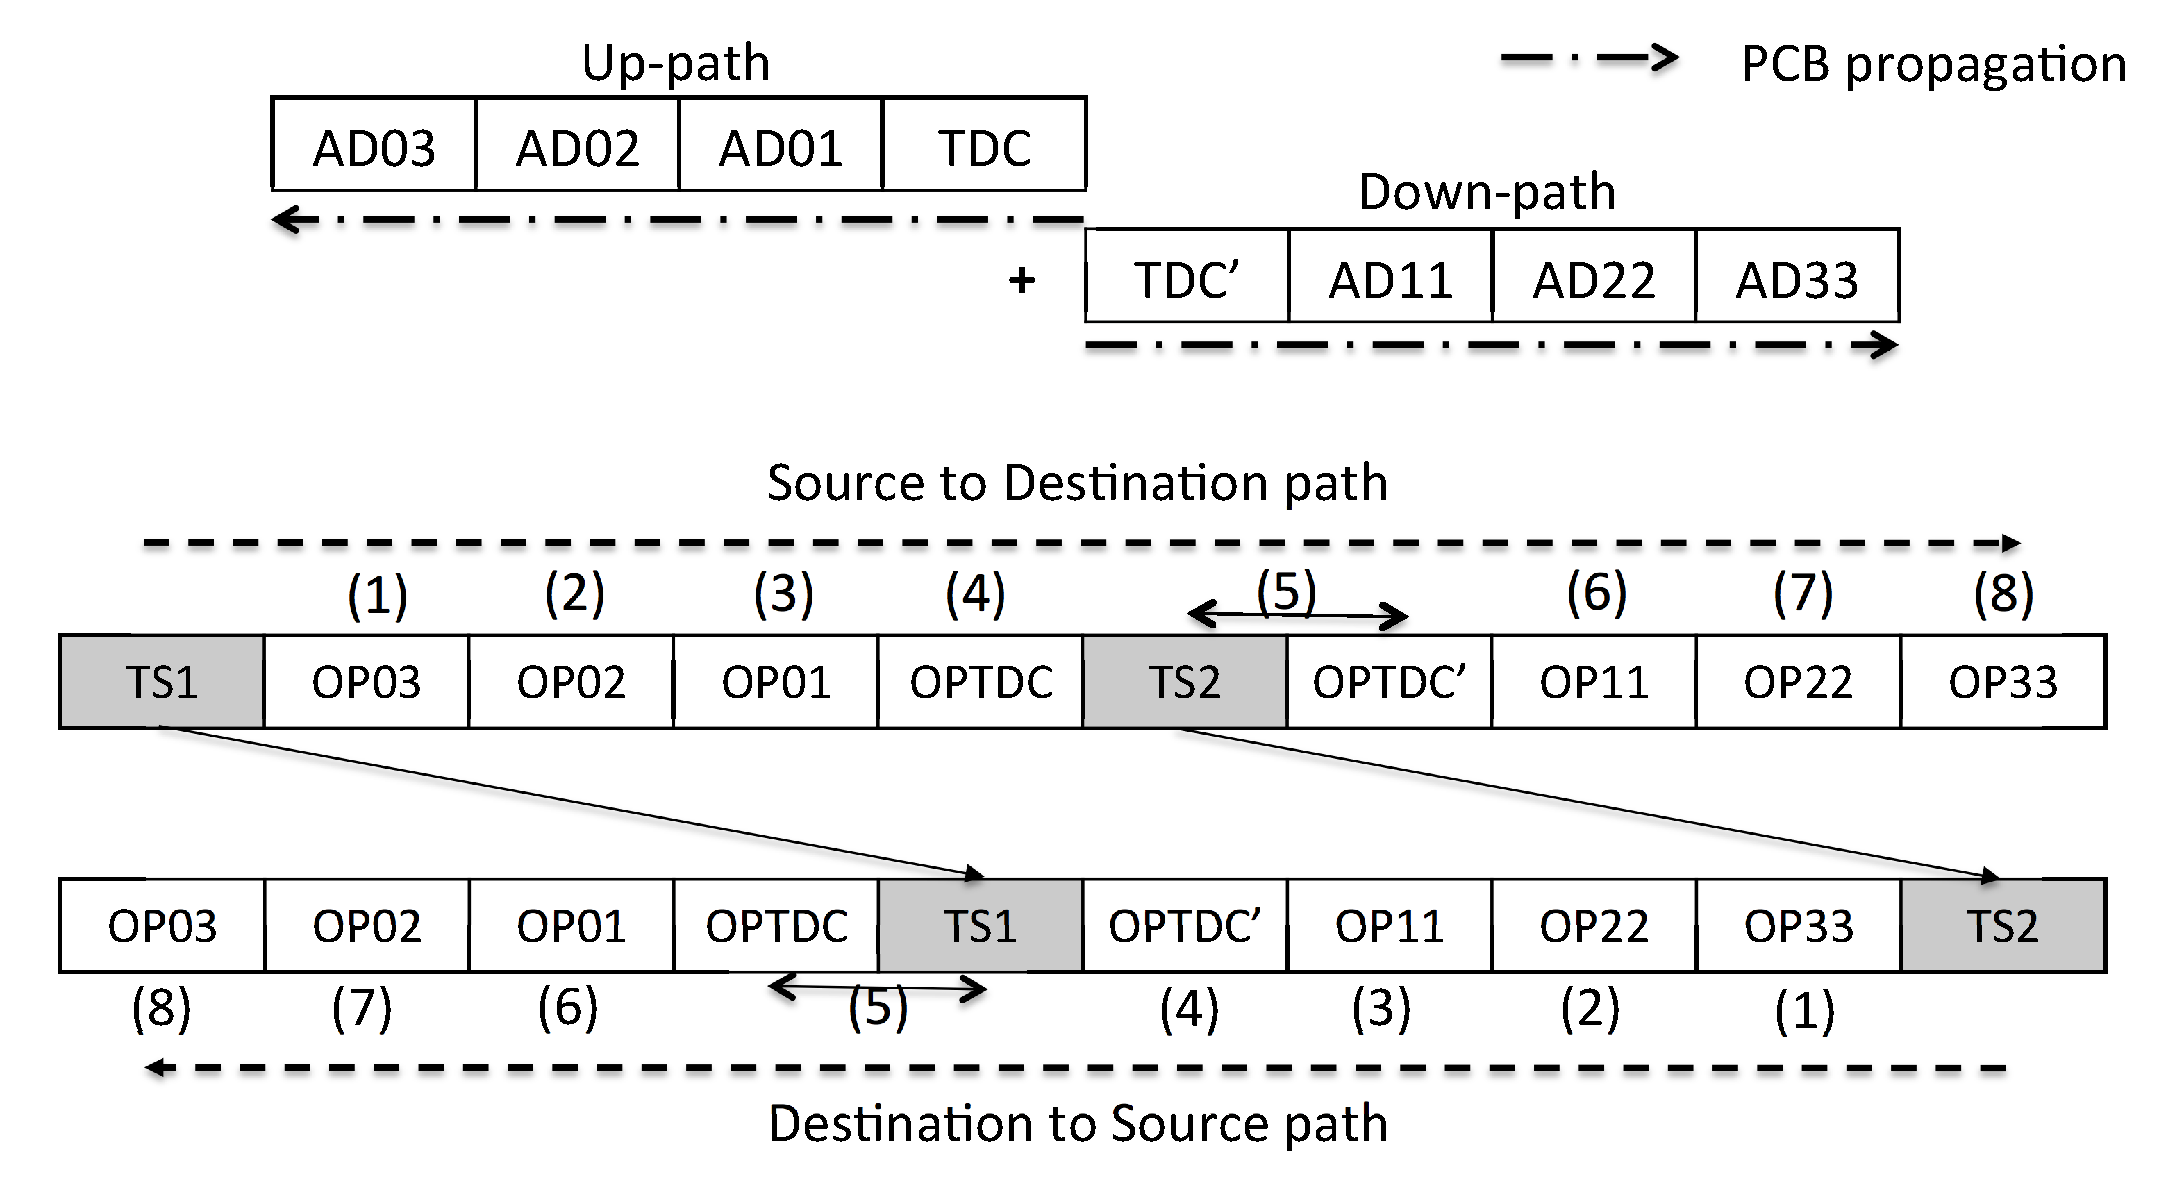
\includegraphics[width=.9\columnwidth]{./fig/nex_fwd1.eps}
\caption{Typical path through \ISDC.}\label{fig:ex-fwd-typical}
\end{figure}

\noindent A sender embeds a series of up-path opaque fields (from its own \AD to \ISDC \AD) and a series of down-path opaque fields (from \ISDC \AD to the destination \AD) into the packet header, thereby constructing a full source to destination path. The up-path opaque field starts with the up-path timestamp (i.e., the special timestamp) so that routers on the path can verify their opaque fields using the timestamp. Similarly, down-path opaque fields start with the down-path timestamp. After embedding the opaque fields, the sender sets the current opaque field pointer (i.e., Curr OF* in Figure~\ref{fig:hdr-common}) to the first opaque field, namely the up-path timestamp. When an \AD sees the special timestamp, the \AD updates the timestamp pointer (i.e., TS*) in the common header and then locates its opaque field by increasing the pointer by 8B. Each \AD on the path locates its own opaque field(s)\footnote{An AD can have multiple opaque fields.} in the common header using the {\em current opaque} field pointer, verifies the opaque field(s): ingress interface ID (i.e., whether the packet arrived at the correct interface) and MAC. If the packet passes the verification, the ingress router increases the opaque field pointer by the amount of its marking, and forwards the packet directly to the egress interface specified in the opaque field. Note that an \AD may have multiple opaque fields that needs to be processed by different routers, hence all routers have to increase opaque field pointer (to the next opaque field) after processing their own part. While all \ADs process opaque field in the same manner, the ingress router of \ISDC \AD (more generally, the ingress router at the end of up-path, which we call the {\em crossover} point) needs to process the opaque field differently. The router has a single egress interface (which an up-path would use as an ingress interface to \ISDC \AD), hence the router has to look at the next opaque field that belong to the first router of the down-path (which would process OPTDC' in the figure), and forwards the packet to the corresponding router. If TDC and TDC' are different \ISDC \ADs, the ingress router of a \ISDC \AD should be able to forward the packet to the next \ISDC \AD. We assume that \ISDC \ADs are well connected and know how to forward packets with each other. When the first router on the down-path receives this packet, the router would see the special opaque field much like the first router on the up-path. Hence, the router would process the packet exactly same way describe before (i.e., update TS* and process its opaque field). The rest of down-path forwarding is exactly same as that of the up-path. 



%2) Up-path and down-path have a common \AD.
\subsection{Up-path and down-path have a common \AD}

\begin{figure}[h]
\centering
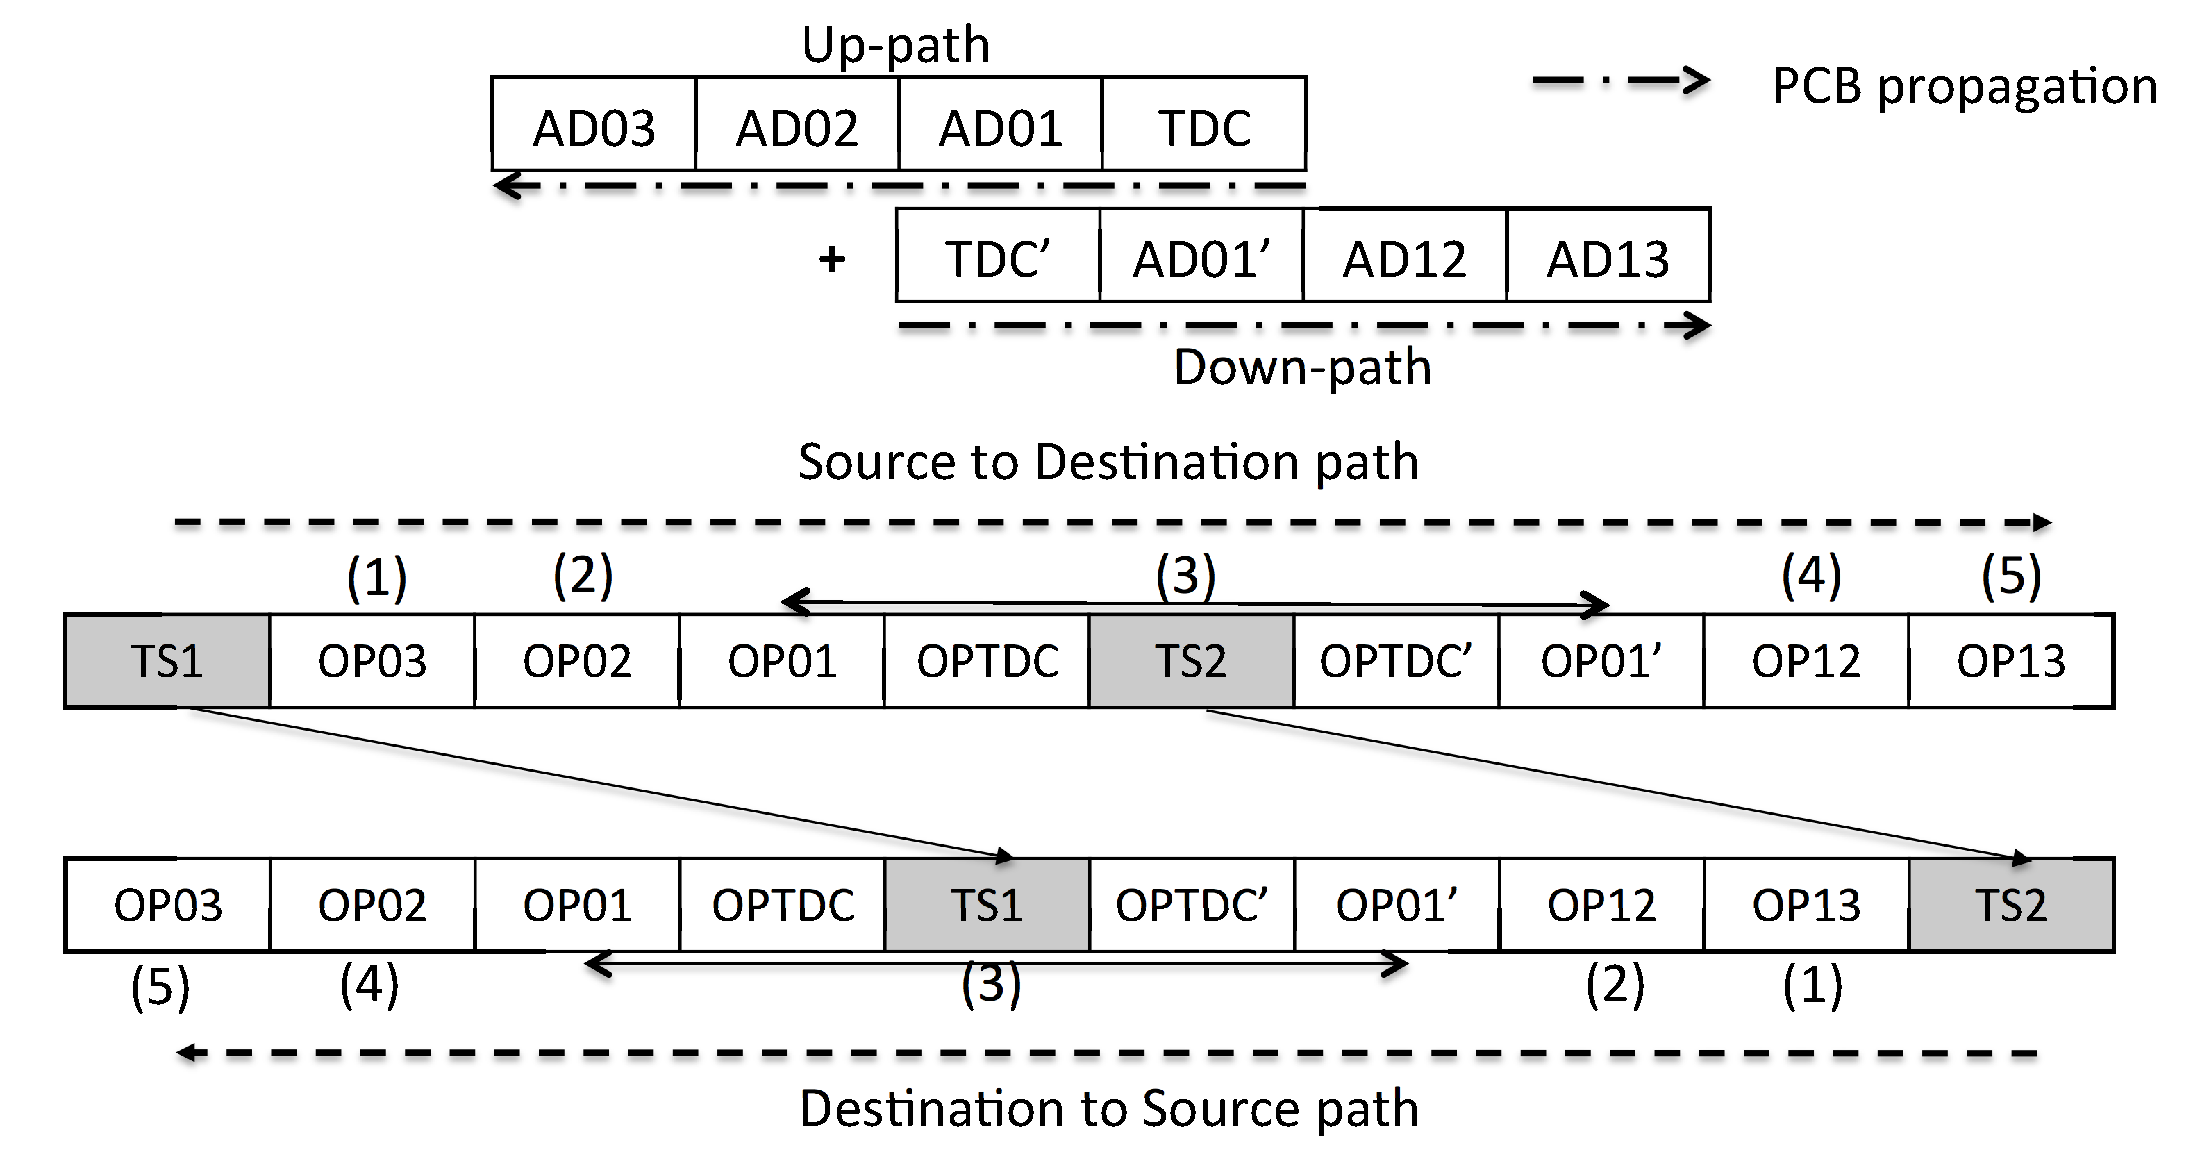
\includegraphics[width=.9\columnwidth]{./fig/nex_fwd2.eps}
\caption{Path composition through a rendezvous point.}\label{fig:ex-fwd-crossover}
\end{figure}

\noindent Figure~\ref{fig:ex-fwd-crossover} shows that \AD 01 is both on the up-path and down-path. In this case, a packet does not need to traverse \ISDC \AD, yet can be directly forwarded to to \AD 12 by \AD 01. To establish a shorter path, the sender sets the first 3 bits of the opaque field of \AD 01 to 110 (viz., Section~\ref{subsec:data-header}), to indicate that the \AD 01 is the common \AD of the up- and down-path (i.e., at the crossover point). If an ingress router finds it is on the crossover point, the router verifies its own opaque field, updates TS* to that of the down-path (which comes after TDC OPTDC in the figure), locates the next opaque field (that belongs to the egress router) coming after next three opaque fields (i.e., its parent, the special opaque field, and another opaque field of its parent), and forwards the packet to the egress interface. The ingress router has to update the Curr OF* to that of the egress router. Also, by having the ingress router update the TS*, the egress router processes this packet. The sender has to embed \ISDC's opaque fields (i.e., OPTDC and OPTDC') into the packet header so that the crossover \AD can verify the opaque fields generated by itself. We note that an \AD generates an opaque field using the opaque field marked by its provider as an input (i.e., by opaque field chaining), hence the provider's opaque field is necessary for opaque field verification.  


%3) Destination \AD is on the up-path.
\subsection{Destination \AD is on the up-path}

\begin{figure}[h]
\centering
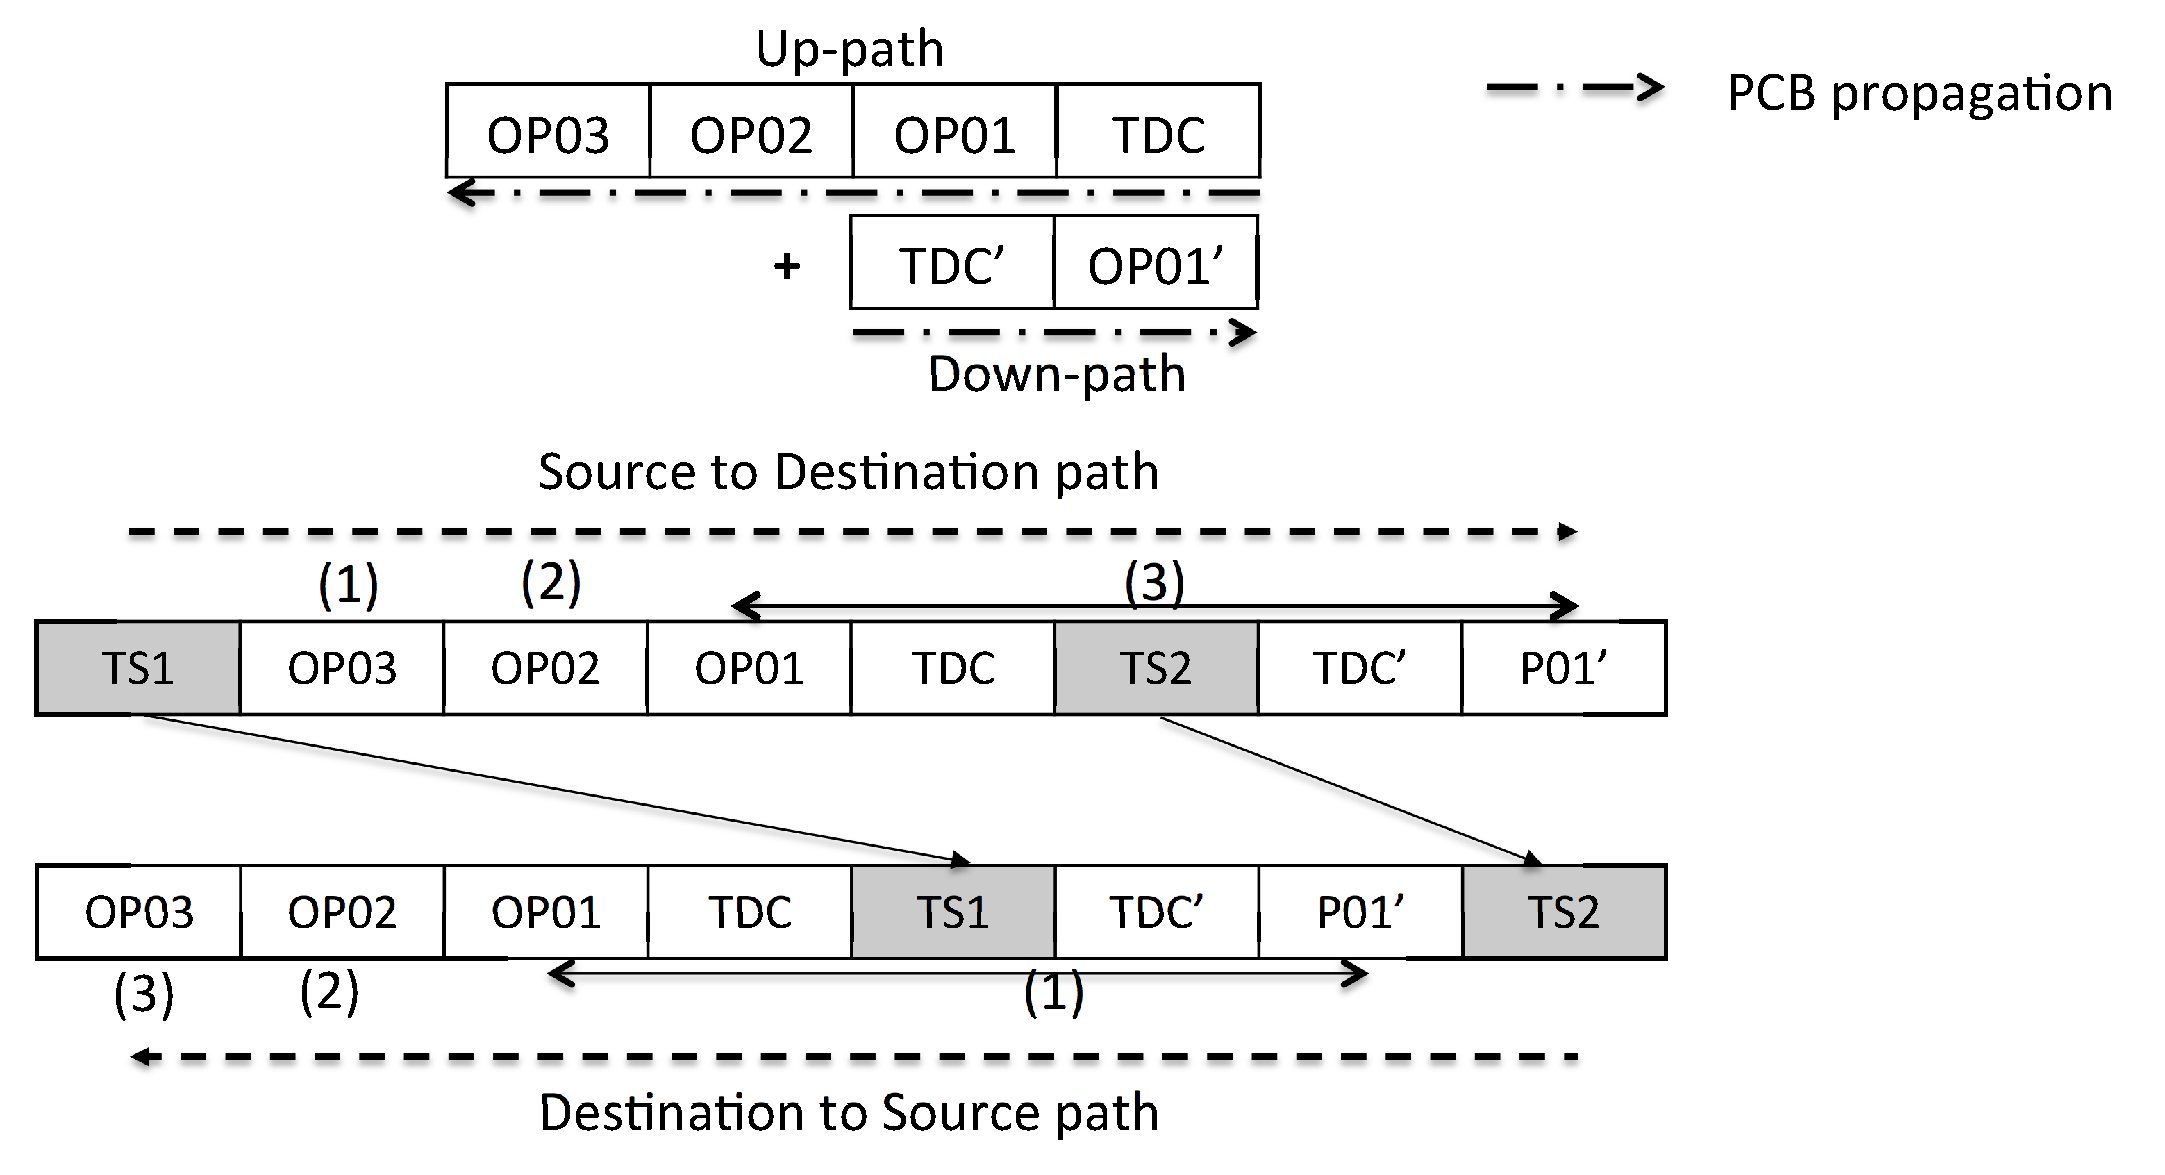
\includegraphics[width=.9\columnwidth]{./fig/nex_fwd3.eps}
\caption{Path composition on the same down-path.}\label{fig:ex-fwd-onpath}
\end{figure}

\noindent If the destination \AD is on the up-path, the sender composes the opaque field in the same way as the crossover scenario, yet the destination \AD is same as the crossover \AD. The destination \AD's down-path opaque field (i.e., OP01' in the figure) still needs to be present in the header so that \AD 01 verifies whether the path is constructed with a valid down-path.

%4) Up-path has a {\em shortcut} to an \AD in down-path.
\subsection{Up-path has a {\em shortcut} to an \AD in down-path}

\begin{figure}[h]
\centering
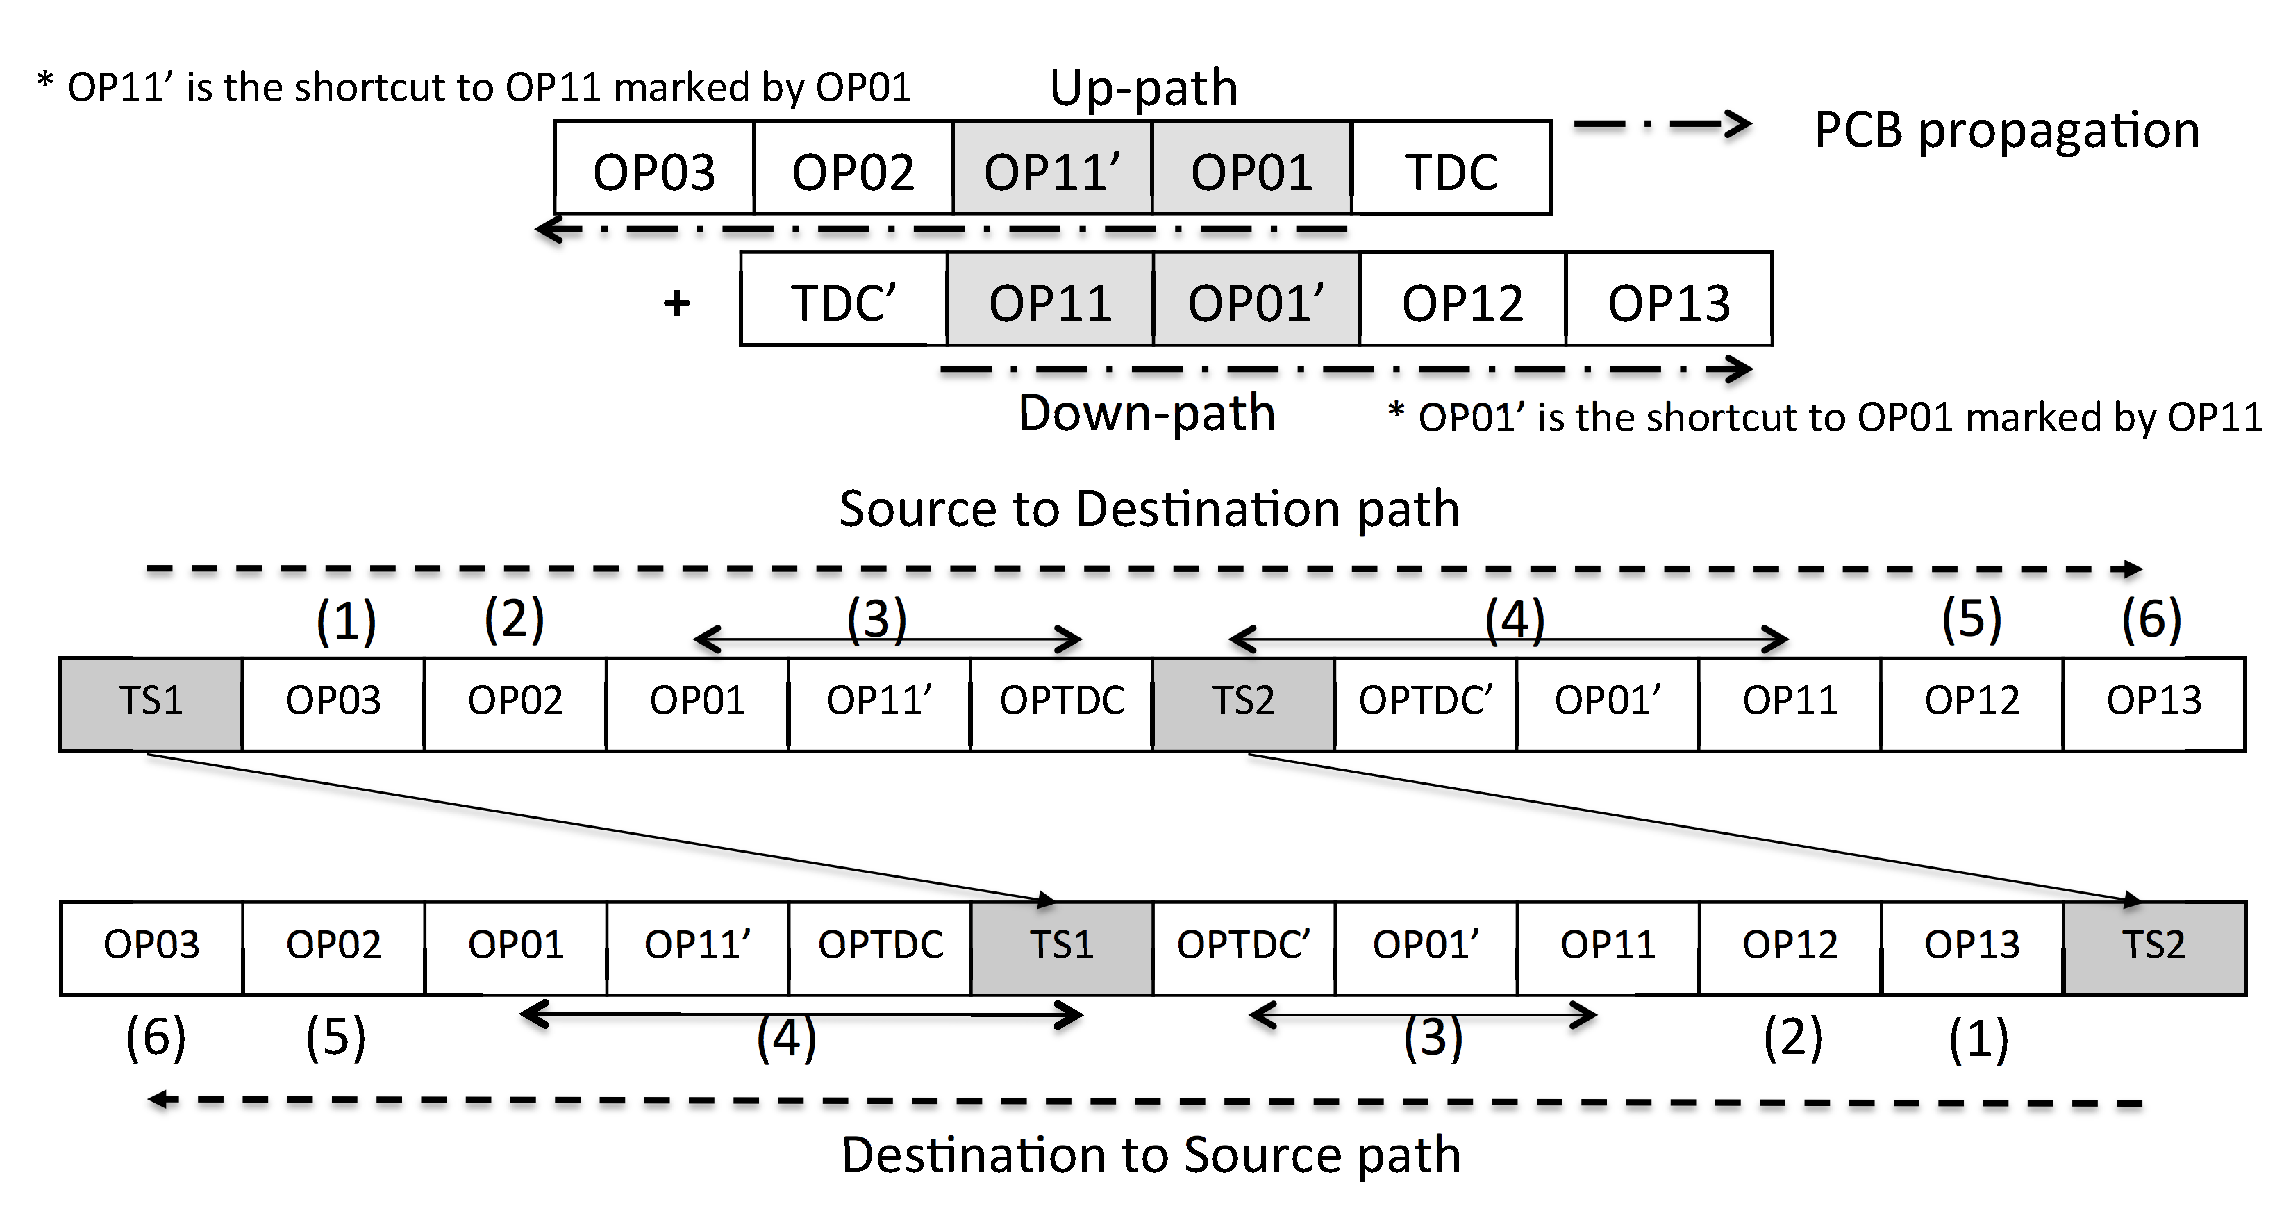
\includegraphics[width=.9\columnwidth]{./fig/nex_fwd4.eps}
\caption{Path composition through a shortcut.}\label{fig:ex-fwd-shortcut}
\end{figure}

\noindent Figure~\ref{fig:ex-fwd-shortcut} shows that during PCB propagation, \AD 01 added OP11' (i.e., shortcut path to \AD 11) to a PCB; and \AD 11 added OP01' (i.e., shortcut path to \AD 01) to a PCB. The sender constructs a shortcut path using the shortcut information (i.e., OP11' in this example) in the up- and down-path. The sender specifies its intent to use the shortcut by setting the first 4 bits of the opaque field (of the shortcut \AD) to 1111. Similar to the previous shortcut scenarios, the sender needs to include OP01 (which is chained to OP11' generation)  and OP11 (which is chained to OP01' generation) in the packet header to enable the \ADs at the crossover point (i.e., AD 01 and AD 12) to verify their opaque fields. However, different from the previous shortcut scenarios, the ingress router of the crossover \AD (i.e., \AD 01) has to skip OP01 and process with OP11' since OP01 is added for AD 02 to verify OP02. The same thing applies to the down-path, yet the first router of the down-path has to update the Curr OF* to that of AD 12 (i.e., OP12) so that the next \AD process the opaque field in the exactly same way as before (i.e., normally).

\begin{comment}
5) Up-path has a {\em shortcut} to an \AD in down-path and different \ISD (i.e., inter-ISD shortcut).
\begin{figure}[h]
\centering
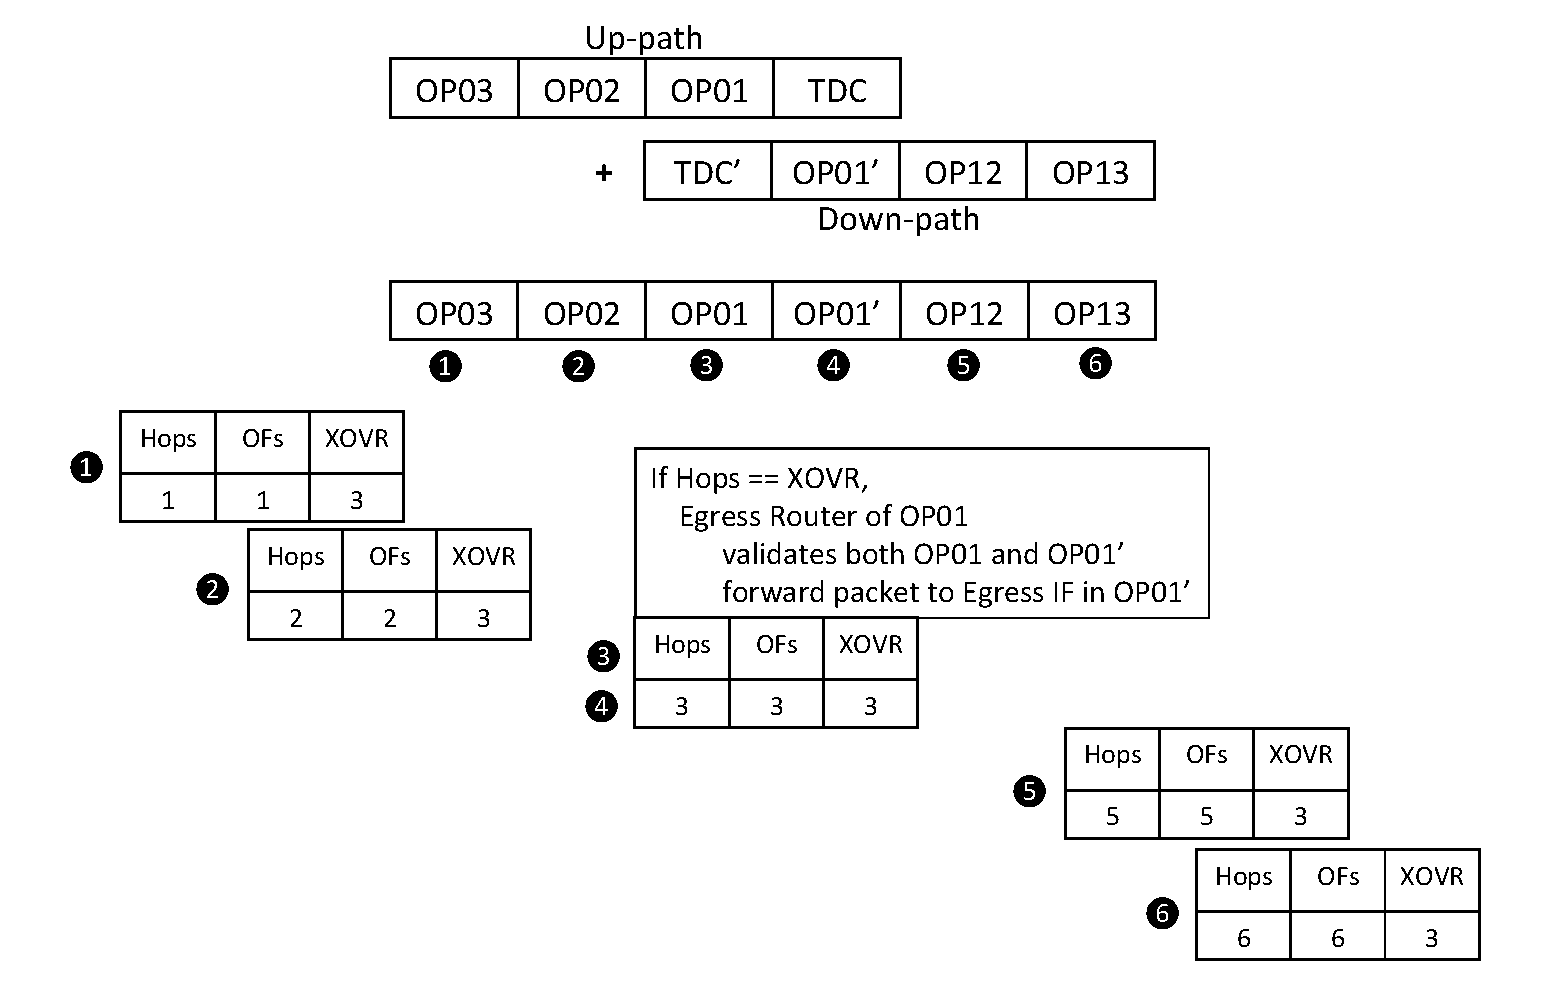
\includegraphics[width=.8\columnwidth]{./fig/ex_fwd5.eps}
\caption{Path composition through an inter-ISD shortcut.}\label{fig:ex-fwd-td-shortcut}
\end{figure}

Inter-ISD shortcut is 

\end{comment}

  \section{SCION Host Architecture}
\index{host architecture}

\subsection{Current host architecture} \chris{this describes the current status and is updated with our progress.}

Figure~\ref{fig:host} provides a high level overview of the SCION host architecture. The components are the following:

\begin{itemize}
\item \textit{Socket}
\index{socket}
In the current setting, the legacy socket code is used. The goal is to provide a SCION socket (AF\_SCION) that takes advantage
of the multiple SCION paths. 

\item \textit{TUN/TAP Interface} is used to enable packet processing in userspace. When applications send data,
the interface captures packets for specific destinations (for which communication proceeds over SCION). To capture
this traffic, routing entries that forward traffic to this interface are inserted in the main routing table. For
incoming traffic from the SCION network, the TUN/TAP interface is used to (re)inject the traffic in the
TCP/IP stack.

\item \textit{Interface between socket and scion\_path}
The details of this interface have to be determined. 
Currently, scion\_path operates as a gateway by encapsulating/decapsulating the SCION header.
The purpose is to give more control to the TCP stack in order to implement a MP-TCP with
higher control levels.


\item \textit{Scion\_path}
The scion\_path daemon runs in userspace and has collected SCION paths (the corresponding OFs) for destination ADs.
For outgoing packets, the daemon inserts the corresponding OFs in a SCION header and then forwards the traffic
to the next SCION node on the path (a SCION border router). For incoming traffic from SCION, the daemon strips
the SCION header and writes the remaining data to the TUN/TAP interface. The interface considers this data as incoming
from the wire and reinjects it in TCP/IP stack. Hence, the actual payload reaches the corresponding applications.
\end{itemize}

\begin{figure}[ht]
\centering
\begin{minipage}{0.85\textwidth}
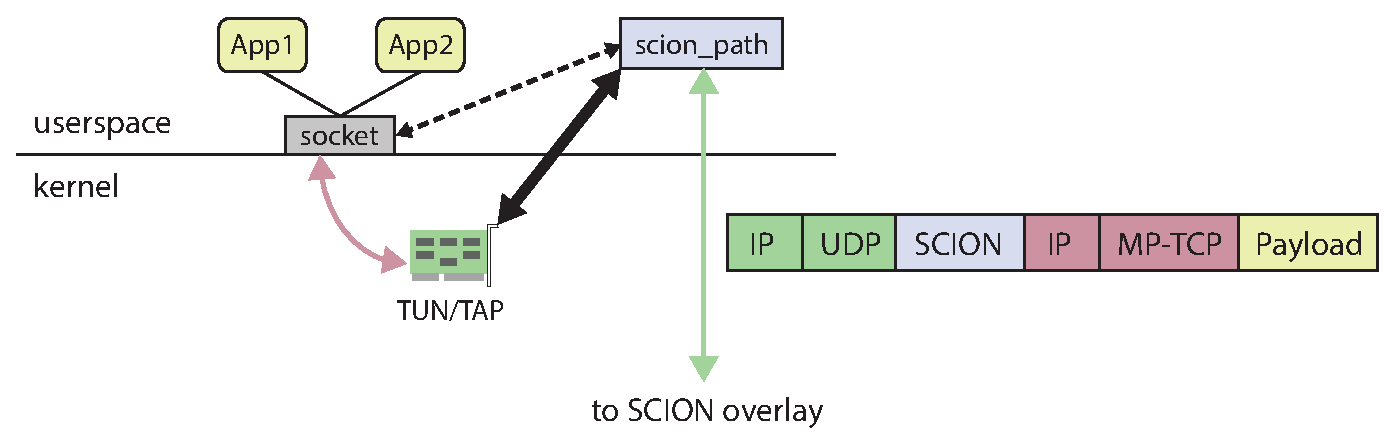
\includegraphics[width=1\columnwidth]{./fig/host2.eps}
\end{minipage}
\caption{Host architecture.}\label{fig:host}
\end{figure}

\subsection{High-level architecture} \chris{outdated, this will change to the final SCION host architecture when it is decided}


Figure~\ref{fig:host} illustrates the architecture of a SCION host.
Normally, a SCION host has the following components.

\begin{itemize}
\item{\em SCION Socket} implements the SCION\_INET socket and provides the SCION socket API to allow user applications to communicate with each other with SCION packets.

\item{\em Name Resolution Client (NRC)} is a permanent user-space process serving all applications that resolves and caches domain names by sending out name resolution requests to Name Resolution Servers in local or remote ADs.

\item{\em Path store in user space} stores half-paths with the associated path metric information. % from PSes within the AD.

%\item{\em Path engine in kernel} contains end-to-end paths with associated information, which are computed according
%to the half-paths in Path engine.

\item{\em SCION layer in kernel} constructs complete SCION packets for applications, and forward the packets according to the routing paths stored in Path
table. Path table contains end-to-end paths with associated
information, which are computed according to the half-paths in Path
store.

\item{\em Multipath TCP module in kernel} allows user applications to use multiple TCP flows to the same destinations over different routing paths stored in path store.

\item{\em Path configuration daemon (PCD) in user space} allows system administrators
to configure path store upon startup, e.g., setting {\em preference
of neighbor ADs} and {\em the number of paths} used to deliver the
packets to the {\em ports} of the {\em destinations}. In the
meanwhile, PCD retrieves half-paths from the PSes within the AD
according to the configurations, and store them in the path store.
Note that, path store parameters are also used to configure
Multipath TCP (MP-TCP) parameters, e.g., the number of paths also
specify the number of subflows for each TCP session, which means
that users can also modify the parameter of MP-TCP to obtain better
application performance. These parameters can be set in application
using the ioctl() system call. Normally, the daemon will set default
values for applications, and system administrators can modify the
default configurations for these applications.
%    (default number of flows, etc) %stores path information.
\end{itemize}

%Figure with host architecture
%- Explain basic components
%  - Host application library
%  - SCION module in kernel
%  - Multipath TCP module in kernel
%  - Path table in kernel, contains half-paths with associated information
%  - Path engine in kernel, contains end-to-end paths with associated information
%  - Path configuration deamon in user space stores path information and
%    configures path table upon startup, configuration of Multipath TCP module
%    (default number of flows, etc)

\begin{figure}[ht]
\centering
\begin{minipage}{0.85\textwidth}
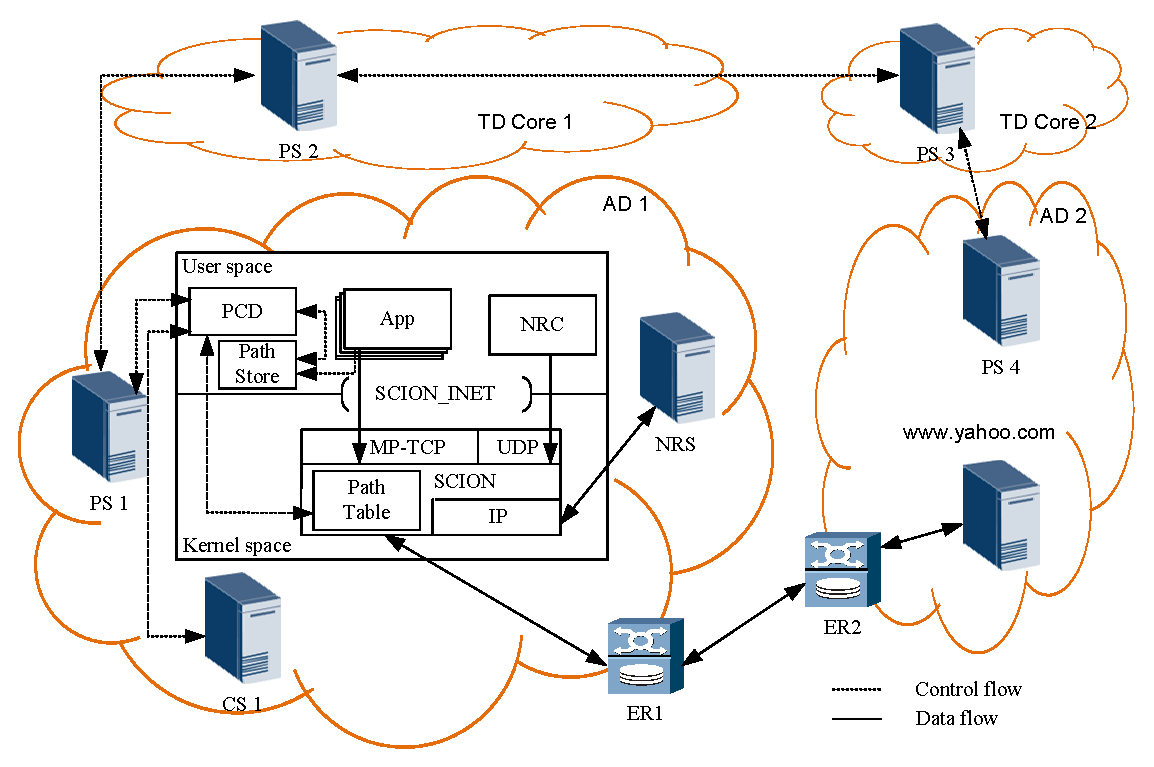
\includegraphics[width=1\columnwidth]{./fig/host.eps}
\end{minipage}
\caption{Host architecture.}\label{fig:host}
\end{figure}

%\begin{figure}[ht]
%\centering
%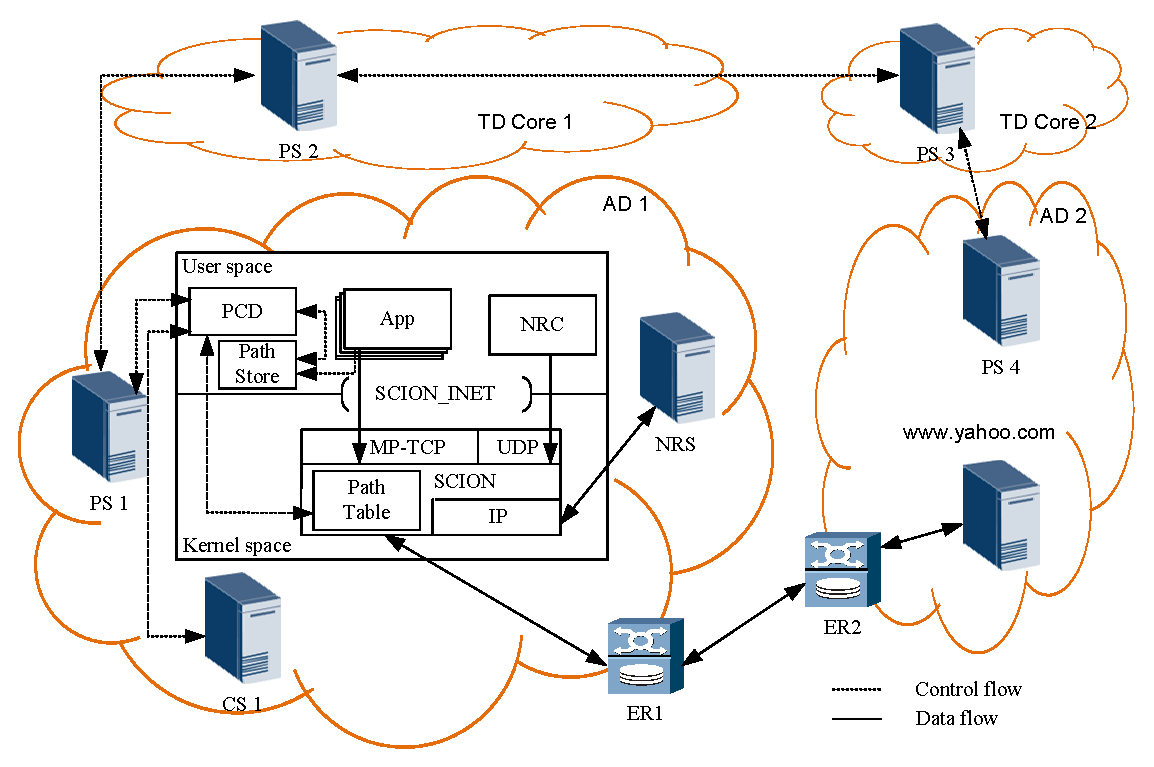
\includegraphics[width=.85\columnwidth]{./fig/host.eps}
%\caption{Host architecture.}\label{fig:host}
%\end{figure}

Each SCION host needs to obtain the correct information of different
servers, e.g., the address of PS, CS, and ER, before sending SCION
packets to the network. Such information is specified in the
topology file. Initially, only a CS address is configured in each
host, and then the host retrieves and loads the topology file from
the CS. After reading the topology file, the host regularly contacts
the CS to check for newer versions of the topology file. Normally,
an AD will have multiple CSes, PSes, and edge routers to obtain
fault tolerance to single CS failure. If any server will be taken
away, the new server will be setup before that.
%Since the
%topology file contains multiple CSes, the host can contact different
%CSes to update its topology file to obtain fault tolerance to single
%CS failure.
Also, the RoT file is initially installed in hosts. If
RoT file is not installed, the host can download it from CSes.

%Configuration of host:
%- Initially, only CS address has to be configured, from which topology file is loaded
%- Later, reading of topology file, contacting CS to check for newer
%  versions. Since topology file contains multiple CSs, we obtain fault tolerance
%  to single CS failure
%- RoT file is initially installed in host, if not, download from CS

\subsection{Example of host-to-host communication}

Now we use an example to illustrate how two end-to-end SCION hosts
can communicate with each other. We assume ISD Cores are operational
and that Name Resolution Server in each ISD Core resolves the
name-to-(local SCION address, AD) binding. In the example, we
suppose that the user, i.e., host in Figure~\ref{fig:host}, intends
to open a TCP connection to www.yahoo.com. Note that, if the host
bootstraps, it will contact the CS for the updated topology file and
then get the addresses of the PS and the ER. The procedure to  UDP
packets is similar, and we do not repeat here.

Applications can obtain name to AD/Address resolution via Name
Resolution Server (NRS) by the {\em getscionhostbyname()} function,
which is extended from the default function gethostbyname() and
implemented in host application library. With the function, host can
reach local NRS by using IP packets. The resolution results of
www.yahoo.com will be stored in the hostent struct. Later, we want
to use SCION anycast to reach NRS within the same domain.

Application opens SCION socket with destination address and AD as
parameters using the function as follows: {\em socket(SCION\_INET,
SOCK\_STREAM, 0))}, where SCION\_INET indicates that the application
wants to generate SCION packets and SOCK\_STREAM denotes that the
application uses TCP connection. After creating SCION the socket,
the ioctl() system call can be used to specify the parameter of the
socket, e.g., which paths within the AD will be preferred. Then, the
application uses the {\em connect()} function with the created
socket and the SCION address specified in the hostent struct as the
parameters to send TCP handshaking packets to the server. If the
socket is successfully connected, the host can read and write
packets via the socket so that it can communicate with the
destination server.

In a low level, all packets generated by the application will be
delivered from the TCP layers to the SCION layer in kernel to
construct complete SCION packets. In the SCION layer, path table
will be lookuped to obtain the correct routing paths for packet
delivery. If the paths are not cached in path table and there does
not exit any entry for the destinations in path store, PCD will
contact local PS to obtain correct paths to the destination. The
communication to local PS is same as communicating with NRS
discussed above. If the destination is in the remote AD, the PSes
will contact the PSes in the ISD core to obtain the paths. As shown
in Figure~\ref{fig:host}, www.yahoo.com is not within the same ISD.
The PSes forwards the path retrieval request to the PSes in ISD
core1, and the PS in ISD core1 will respond to the request with the
paths that are retrieved from ISD core2. Normally, PCD will retrieve
paths from the PS for different destinations and record them in path
store once the applications are installed. To allow applications and
system administrators can specify path selection preference, each
path in path store will be stored with more path quality
information, e.g., path bandwidth and delay.
%launched, and the
%destination addresses are recorded in PCD when the application are
%installed.
%PCD , the path store will retrieve the
%paths for the application and periodically contact update the paths.
Later, we will add APIs and command lines to enable configuring path
selection policies in path table by system administrators.

Path store will build end-to-end paths by joining up-paths and
down-paths that are retrieved from the PS according to routing
selection policies, and insert the result of end-to-end paths to
path table. The SCION layer lookups the path table and gets the
end-to-end paths to deliver the packet, and then construct the SCION
packet by putting the complete path information in the SCION header. %If the destination
%within the same AD, the SCION packet will be delivered to the
%destination according to the information in SCION header. Otherwise,
The packet will be sent to ER for further delivery. For example, as
shown in Figure~\ref{fig:host}, the packets to www.yahoo.com will be
sent to ER2, and then finally gets to the server.

To fully utilize the features of SCION, the future SCION\_INET
socket implementation can build end-to-end paths according to the
QoS parameter and routing policy parameters, which are configured by
application developers by using the ioctl() system call, or system
administrators by using path configuration daemon, based on the
local network performance, the application performance requirements,
and path selection preference. In the meanwhile, SCION can also
allow system administrators to directly specify entire end-to-end
paths for the applications that can be identified with the
destination addresses and the corresponding ports.
%\qi{Normally, applications cannot know the path
%information and user preference in each host so that they may not
%choose correct paths for users. Instead, users can easily use these
%information. So, I think it would be good to configure these stuffs
%in the path configuration daemon by users, e.g., according to the
%network performance and the user preference.}

%- later API: QoS parameters, routing policy parameters
%- even later API: entire end-to-end paths

%AD to path resolution via local Path Server (local PS) if destination AD
%information is not cached. Contacting local PS is done same as contacting NRS
%above. Add half-paths to path table
%- Maintain a default path table in the Kernel, but later, add API that enables
%  configuring path selection policies.
%- Define the path table structure that reflects path quality (e.g.,
%  bandwidth, delay, and so on)

%Build an end-to-end path by joining up-paths and down-paths from path table,
%insert end-to-end paths to path engine

%Create a SCION packet

%Send a packet using the SCION module, sent to ER in case destination is in
%different AD.

\subsection{Implementation Details}

\subsubsection{Overview: Implementation in Linux}

We implement the Path Store and PCD in the Linux user space (see
Figure~\ref{fig:host}. Other components are implemented in the
kernel space. We implement a SCION socket called the SCION\_INET
family to allow applications to create SCION packets, implement a
SCION layer in the networking stack, which lookups the path table
and constructs SCION packets, and a virtual network device, sciond,
which is used to transmitting and receiving SCION packets.
Figure~\ref{fig:kernel} illustrates the implementation of SCION
hosts in the kernel space. If an application create a SCION socket,
and the generated packets will be go through the TCP and the UDP
layers as normal. Before the packets get into the IP layer, the
packets will be hooked at the netfilter NF\_INET\_LOCAL\_OUT hook.
All packets labeled with SCION\_SOCKET family will be injected into
the SCION layer. The SCION layer will replace the IP headers with
the SCION header, and construct complete SCION packets and deliver
them to sciond. For the case of receiving packets, any SCION packets
getting to sciond will be delivered to sciond. In sciond, the SCION
headers will be replaced with IP headers, and the packets will go
through the legacy network and transport layers and be delivered the
applications.

\begin{figure}[ht]
\centering
\begin{minipage}{0.65\textwidth}
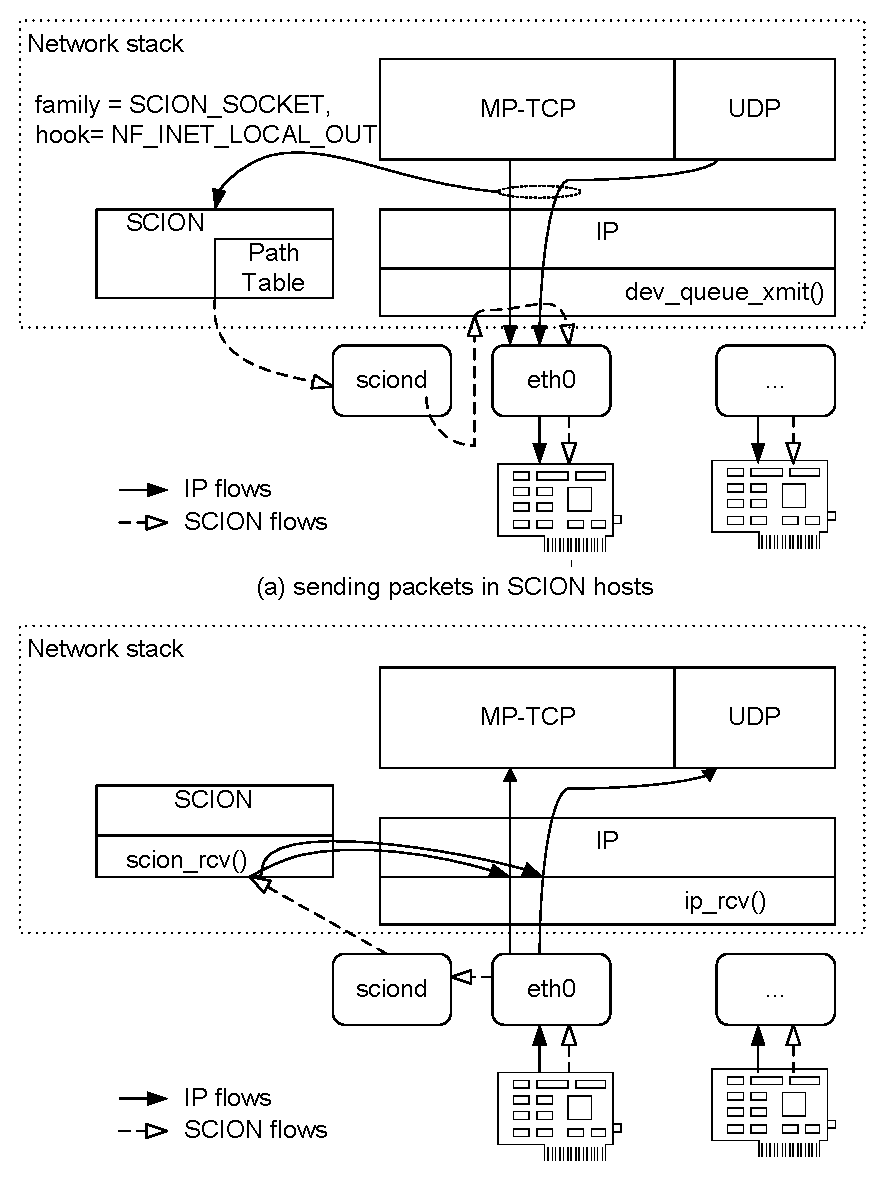
\includegraphics[width=1\columnwidth]{./fig/host_kernel.eps}
\end{minipage}
\caption{SCION implementation in Linux kernel.}\label{fig:kernel}
\end{figure}

The advantage of the implementation design is oblivious because we
cam enable SCION in the end host without any modification in
applications and the transport layer. Therefore, legacy applications
can easily use the SCION packets to communicate with the
destinations by configurations in PCD. In the meanwhile, the SCION
hosts can fully share the benefits of the existing mechanisms in the
current networking stack, e.g., we can directly use MP-TCP to enable
packet delivery over multipaths. Moreover, SCION hosts can achieve
much better performance with multipath packet delivery than the
traditional MP-TCP in the legacy hosts by enabling fine-grained path
selections according the path metric piggybacked in the path
announcements, i.e., beacons.

\subsubsection{Key Modules}

To fully implement SCION host architecture, SCION hosts have the
following blocks.

\begin{itemize}
\item{Implementation of the SCION\_INET Socket.}\ \ We will implement the following prot\_ops
structs and the related functions to enable the SCION socket API. We
only need to define a new family name and implement a scion\_ioctl
system call to allow application developers to specify path
selection policies in the applications, e.g., preferring paths
within the same ISD. Other functions are not changed as the
traditional inet\_stream\_ops and inet\_dgram\_ops structs,
respectively.

\begin{footnotesize}
\begin{lstlisting}[language=C]
 struct proto_ops scion_stream_ops = {
          .family         = SCION_INET,
          .owner          = THIS_MODULE,
          .release        = inet_release,
          .bind           = inet_bind,
          .connect        = inet_stream_connect,
          .socketpair     = sock_no_socketpair,
          .accept         = inet_accept,
          .getname        = inet_getname,
          .poll           = tcp_poll,
          .ioctl          = scion_ioctl,
          .listen         = inet_listen,
          .shutdown       = inet_shutdown,
          .setsockopt     = sock_common_setsockopt,
          .getsockopt     = sock_common_getsockopt,
          .sendmsg        = tcp_sendmsg,
          .recvmsg        = sock_common_recvmsg,
          .mmap           = sock_no_mmap,
          .sendpage       = tcp_sendpage,
          .splice_read    = tcp_splice_read,
 }
\end{lstlisting}

\begin{lstlisting}[language=C]
 struct proto_ops scion_dgram_ops = {
          .family         = SCION_INET,
          .owner          = THIS_MODULE,
          .release        = inet_release,
          .bind           = inet_bind,
          .connect        = inet_dgram_connect,
          .socketpair     = sock_no_socketpair,
          .accept         = inet_no_accept,
          .getname        = inet_getname,
          .poll           = udp_poll,
          .ioctl          = scion_ioctl,
          .listen         = sock_no_listen,
          .shutdown       = inet_shutdown,
          .setsockopt     = sock_common_setsockopt,
          .getsockopt     = sock_common_getsockopt,
          .sendmsg        = inet_sendmsg,
          .recvmsg        = sock_common_recvmsg,
          .mmap           = sock_no_mmap,
          .sendpage       = inet_sendpage,
 }
\end{lstlisting}
\end{footnotesize}

\item{Implementation of the SCION Layer and Virtual Device.}\ \
The SCION layer needs to lookup path table and deliver SCION packets
from and to the transport layer. Normally, we hook all packets from
the transport layer, and redirect the packets to the SCION layer if
the packet family specified in the sk\_buff struct is the
SCION\_INET family. The SCION layer lookups the path table to
retrieve the path information,
i.e., the Opaque information. %If the packets are for the remote
%destination,
and then replaces the IP header with the SCION headers. %will be
%inserted into the packets and the output device in the sk\_buff
%structure.
Then packets will be passed to the virtual device to finish packet
transmission. For the case of receiving packets, all SCION packets
will be delivered to the SCION packet handler, i.e., scion\_rcv(),
that fills in the IP headers in the sk\_buff struct, and then the
packets will delivered to the transport layer through the IP layer
for the purpose of enabling the normal packet processing procedure.
%If
%there does not exist any path entry in path table,
%tcp\_transmit\_skb() will directly pass the packets to
%ip\_queue\_xmit() for normal IP packet processing.

\item{Implementation of the Path Configuration Daemon.}\ \  Path PCD uses IP
packets to communicate with CSes to retrieve the topology file and
to contact PSes to request paths to the destinations. %In SCION
%hosts,
The retrieved up- and down-paths are stored in the path store (in
the user space). To avoid the delay of paths retrieval during
application startup, PCDs can pre-retrieve all half-paths for the
applications according to the system administrators' configurations.
%We can
%implement a Linux kernel module to create /proc nodes for all SCION
%related information. Then, all path configuration operations
PCD can directly create and modify path selection policies for
different destinations. We also allow PCD to directly modify the
end-to-end paths in the path table via the scion\_link socket that
is extended from the netlink socket.
%provided in path
%configuration daemon can be enabled by reading or modifying the
%corresponding node in the /proc filesystem. Later, we can add some
%system calls in the kernel so that the path configuration daemon can
%use the system calls to enable more fine-grained path configurations
%policies.
Moreover, by specifying the destination addresses and the port
number in PCD, legacy applications can also use SCION packets to
communicate with the corresponding destinations. Note that, path
selection policy configuration can be also enabled in applications
by using the ioctl() system call.
%, and the computed
%end-to-end paths in path table are maintained in Linux kernel

\item{Implementation of the Path Store.}\ \ It maintains up- and
down-paths learned from PSes, and compute the end-to-end paths
according to path configuration policies. The result end-to-end
paths will be inserted in the path table in the kernel space. %We
%implement a new socket called scion\_link that is extended from the
%netlink socket
The computed end-to-end paths in the path store will be updated to
the path table by using the scion\_link socket. The details of the
Path Store implementation and path selection policies will be
discussed in the next chapter.

\end{itemize}

%%% Local Variables:
%%% mode: latex
%%% TeX-master: "paper"
%%% End:

  %
\chapter{Host-to-host Communication Example}



%%% Local Variables: 
%%% mode: latex
%%% TeX-master: "paper"
%%% End: 

  \chapter{Gateway}
In this section, we describe a SCION gateway, which bridges between a SCION network and an IP network. SCION gateways enable (1) connecting two physically separate SCION networks via IP networks, and (2) IP clients to communicate with/through a SCION network without modifying their protocol stack (i.e., transparently). In essence, SCION gateways integrate SCION networks with IP networks in a seamless manner, thereby enabling incremental and independent adoption of SCION architecture. 

\begin{figure*}[ht]
\centering
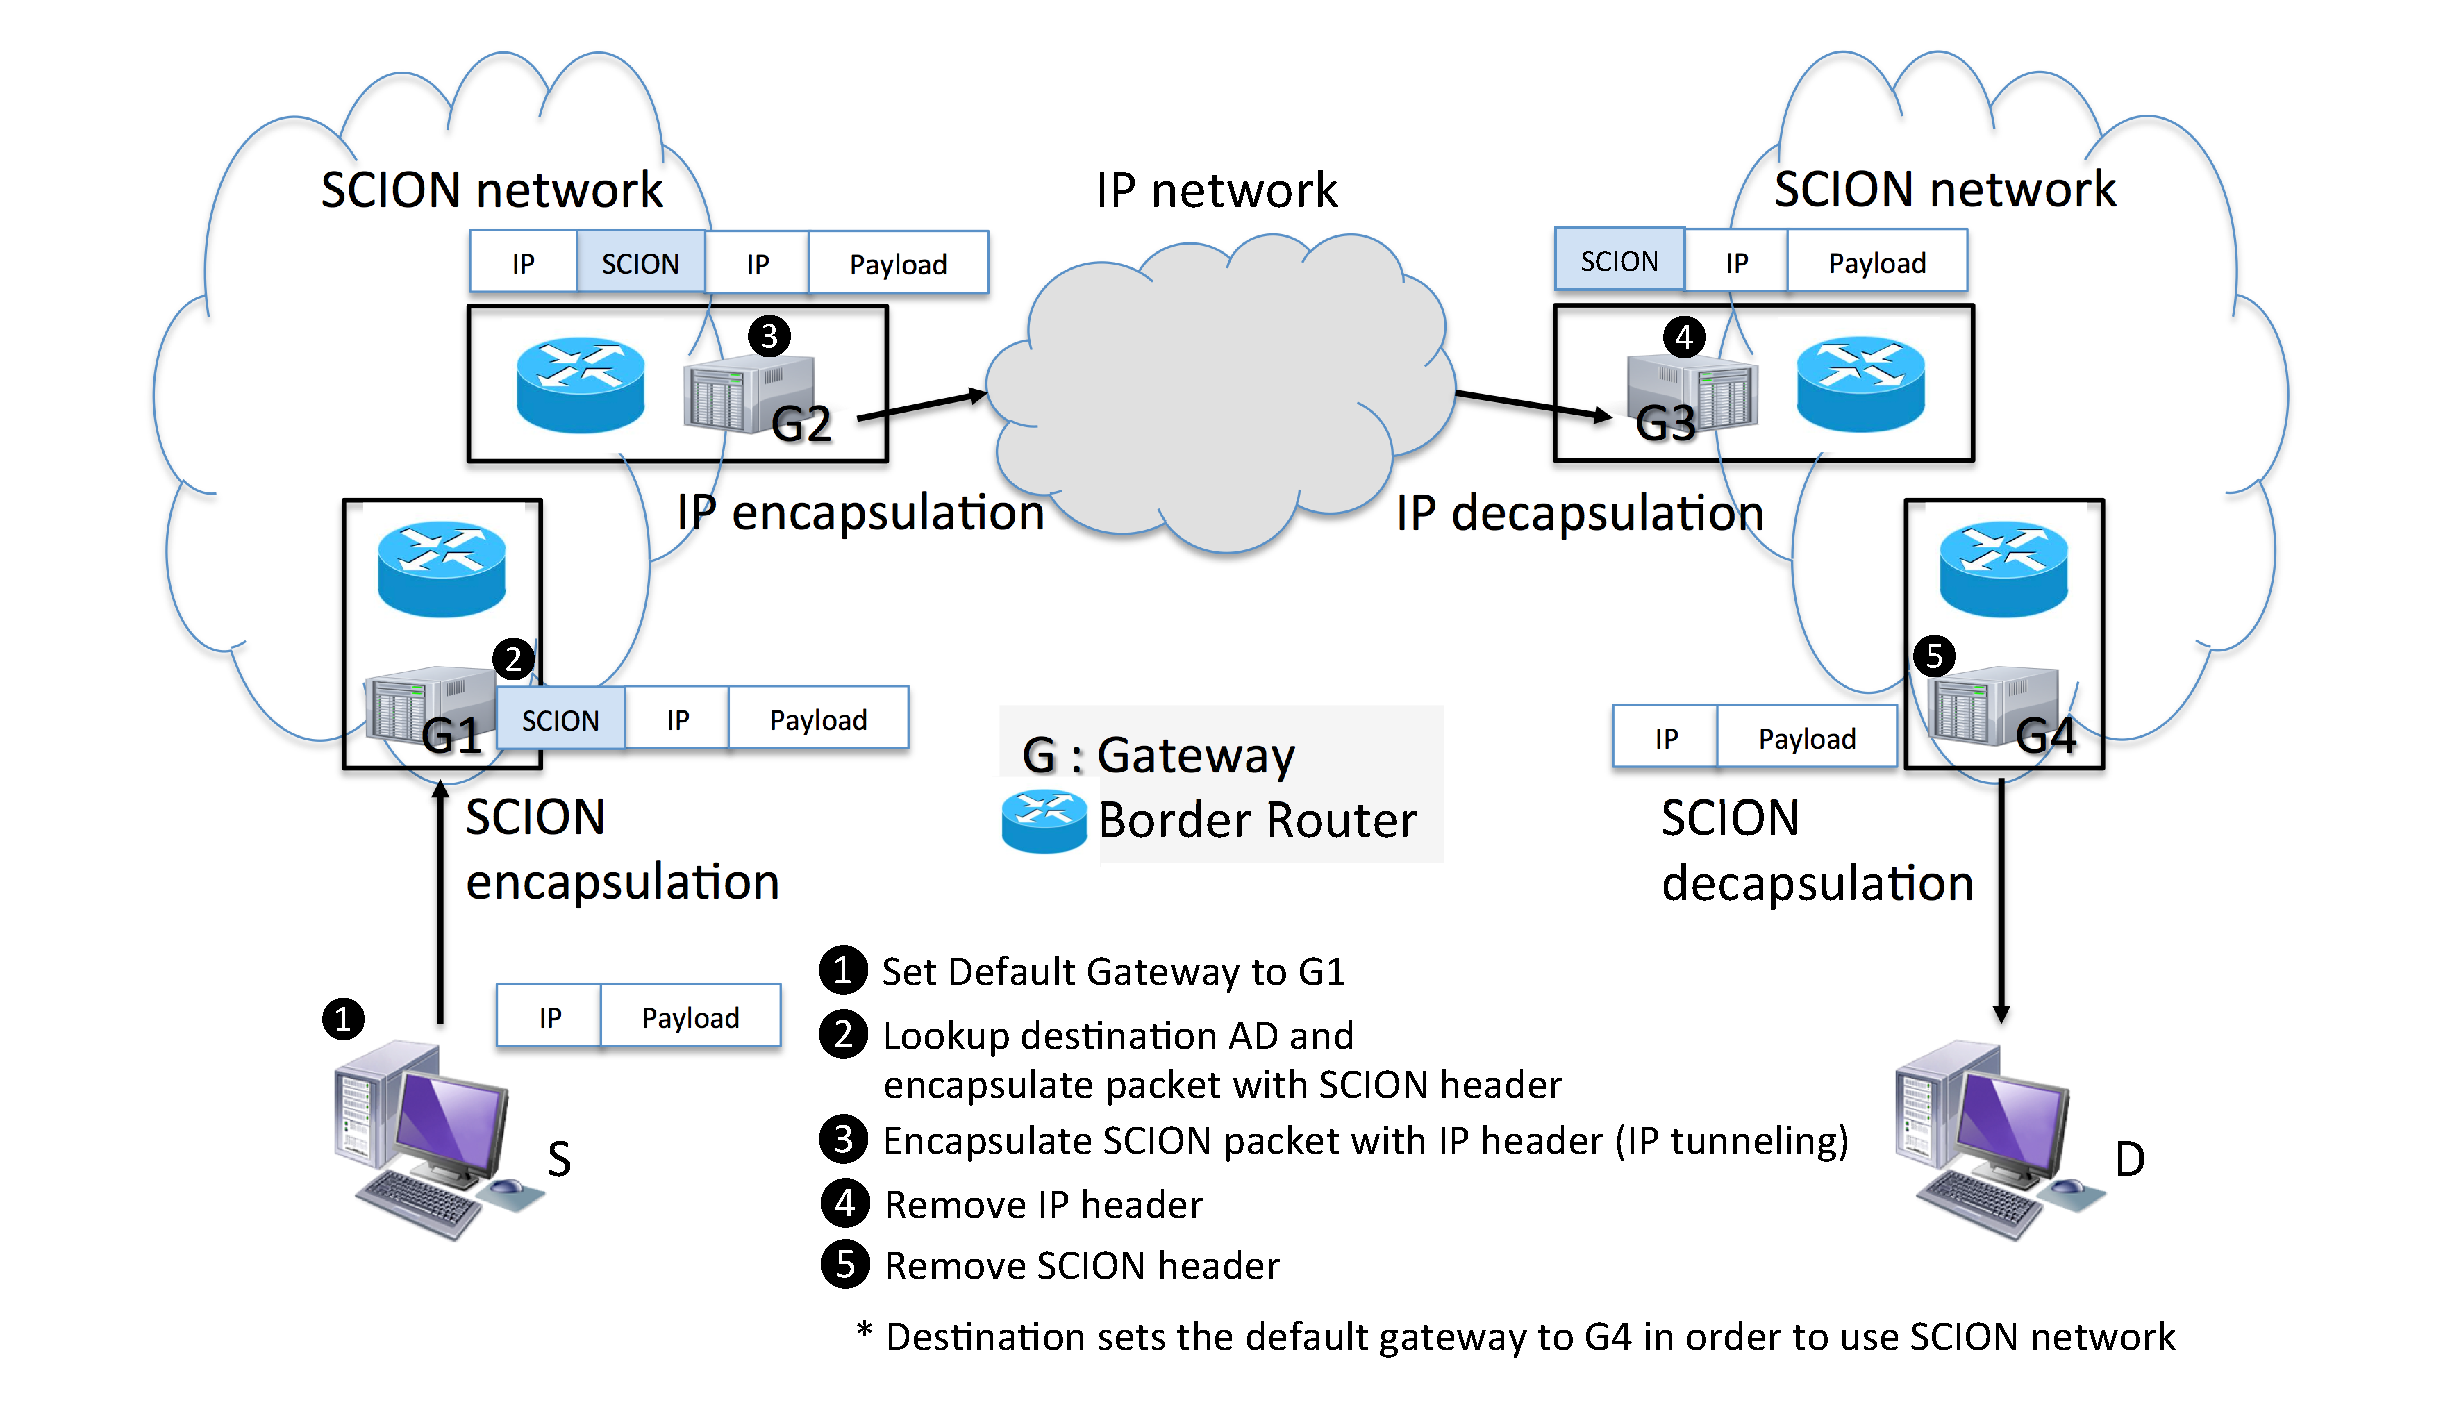
\includegraphics[width=\columnwidth]{./fig/gateway.eps}
\caption{SCION Gateway.}\label{fig:gateway}
\end{figure*}

\section{Gateway for IP tunneling}
Two SCION networks can be connected via IP network using SCION gateways. For this purpose, SCION gateways encapsulate a SCION packet with IP header, where the sending gateway sets the source IP address to its own address and the destination IP address to that of receiving gateway. Once a SCION gateway receives a packet from another SCION gateway~\footnote{Each gateway has the list of SCION gateways in its configuration file}, it removes IP headers and forward packet to the SCION network to which it is connected. That is, SCION gateways have at least two interfaces that are connected to two different networks (i.e., SCION and IP networks) and forward SCION packets through {\em IP tunnels}. Tunneling is simply configured as: the sending gateway has the map between an outgoing SCION interface (to itself) and the IP address of the corresponding destination gateway to which the incoming SCION interface is connected; the receiving gateway has the list of the IP addresses of sending gateways.The receiving gateway, once it removes a packet's IP header, is able to determine the SCION interface to which the packet should be place. We name this type of gateway as {\em IP tunneling} SCION gateway. The steps 3 and 4 in figure~\ref{fig:gateway} illustrate this IP tunneling. 

\section{Gateway for IP clients}
All IP-based applications can communicate via SCION network by setting their default gateway to the IP address of SCION gateway. For this purpose, SCION gateways, on receiving a packet from the IP interface, look at the destination address of the packet, resolve the address to the destination AD, and encapsulate the IP packet with the SCION header. As a result, this gateway, named {\em last-mile gateway}, enables IP clients to use SCION networks without changing its protocol stack. The destination gateway simply removes the SCION header and forward the packet to the destination address in the IP header. In this case, the whole IP packet is treated as a payload by SCION routers and only is interpreted by {\em last-mile} SCION gateways. Steps 2 and 5 in Figure~\ref{fig:gateway} illustrate packet processing by the last-mile SCION gateways.


  \newcommand{\sps}{SCION PathStore\@\xspace}
\newcommand{\pse}{path-selection engine\@\xspace}
\newcommand{\PSE}{Path-selection Engine\@\xspace}
\newcommand{\qs}{queue snapshot\@\xspace}
\newcommand{\QS}{Queue Snapshot\@\xspace}
\newcommand{\sq}{SCION queue\@\xspace}
\newcommand{\SQ}{SCION Queue\@\xspace}
\newcommand{\BPS}{Best-path Set\@\xspace}
\newcommand{\bps}{best-path set\@\xspace}
\newcommand{\stride}{STRIDE\@\xspace}

\chapter{Path Store}
In this section, we describe {\em \bf SCION PathStore}, a data structure for storing SCION paths. We design \sps such that it would be used by both \BS and \CS.
The basic functionality of \sps is to store PCBs (which correspond to
SCION half-paths) in the local storage and to provide a set of paths
that best satisfy certain requirements.

{\bf \BS: } \BS stores all PCBs received from its upstream \ADs and at
each PCB propagation epoch, selects the best $k$ paths to propagate to
its customer \ADs. For this purpose, \BS evaluates the {\em path
  fidelity} (viz., Section~\ref{subsec:pcb_selection}) of each path
and maintain a list of $k$ paths that have the highest fidelity for
each customer \AD.

{\bf \PS: } \PS stores all up-paths received from the local \BS and on a client request, provides the best a set of paths that satisfy the client's request.

\begin{figure*}[th]
\centering
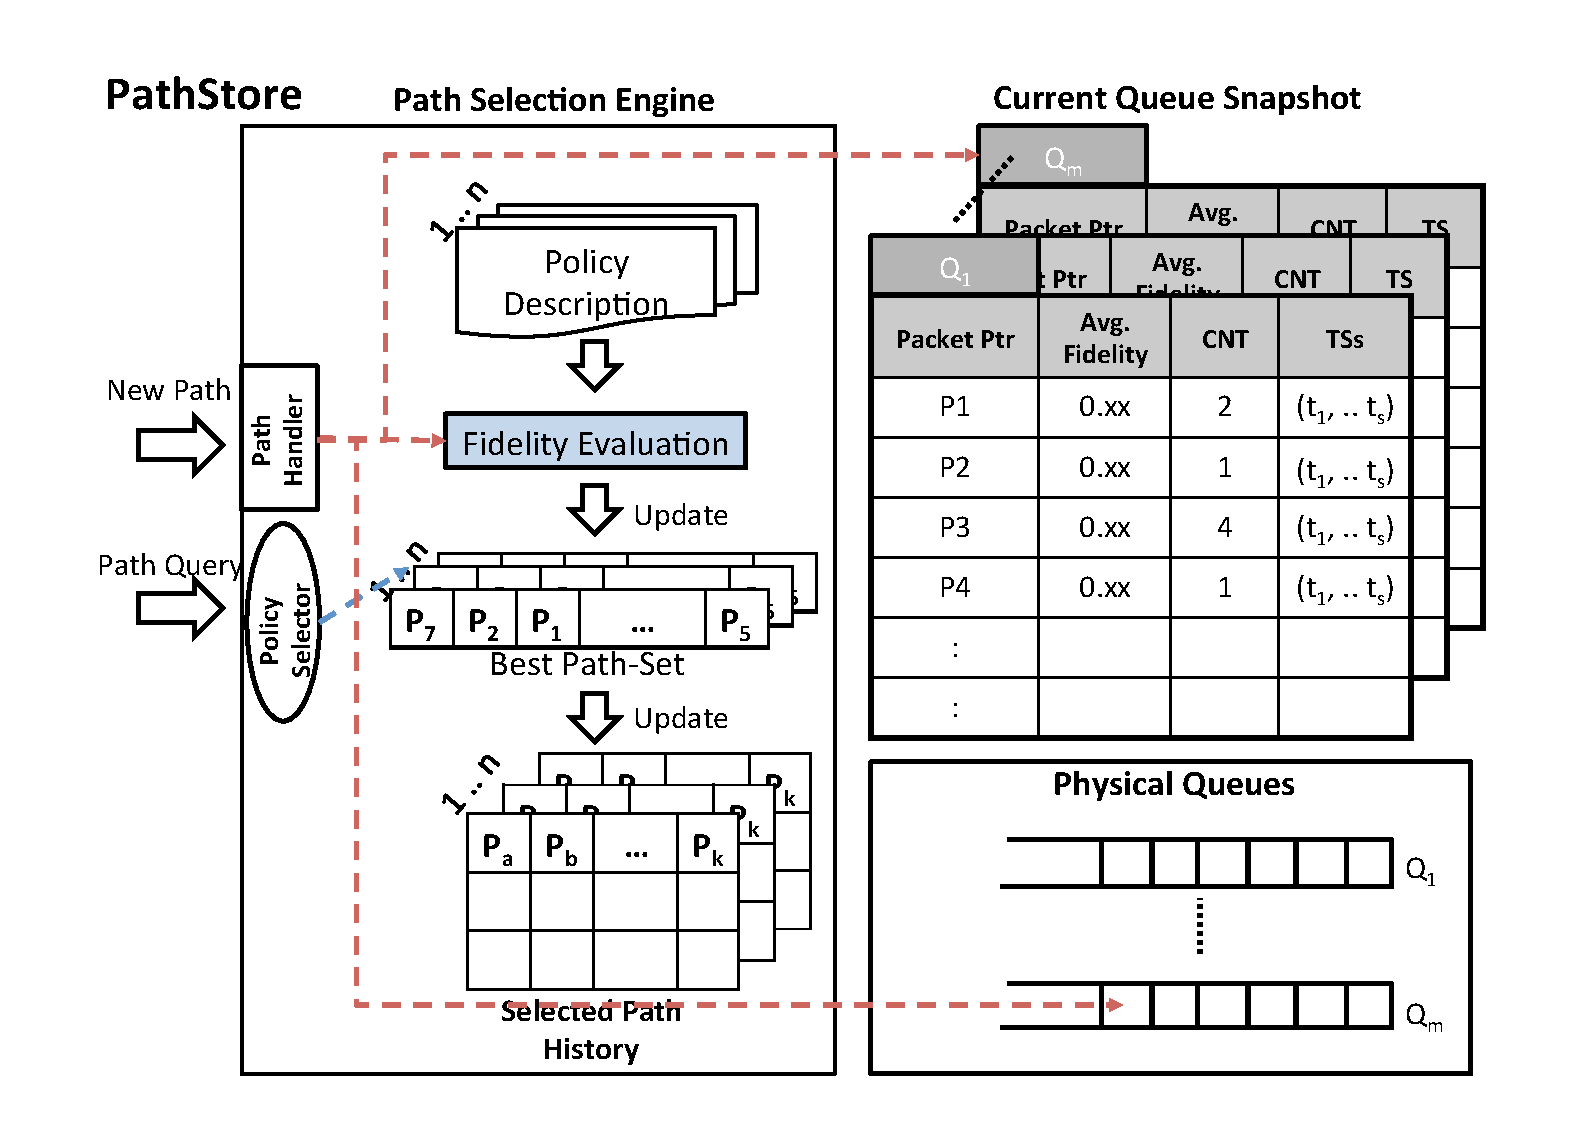
\includegraphics[width=.9\columnwidth]{./fig/path_store.eps}
\caption{Path Store.}~\label{fig:path_store}
\end{figure*}

\section{Overview}
\sps consists of three parts in large, which are \pse, \qs, and \sq. 

{\bf \PSE: } \PSE has a list of policies that describe the preference
of paths and a list best-path sets that correspond to individual
policies. For a new path, the \pse evaluates the path fidelity based
on each policy and adds this path to the corresponding best-path
set. The best-path set is sorted in the decreasing order of fidelity,
and the size of the best-set can be configured. For example, \BS sets
the size to $k$, where $k$ is the number of paths that would be
propagated to its customer \AD. \PSE stores the list of the selected
paths at a specific time in the path history table, by which the \pse
can evaluate path properties dependent on previous selection. Such
history-dependent path properties include path freshness and path
disjointness, as detailed in the next subsection. Storing exact copies
of selected paths in the path history table enables accurate
evaluation of history-dependent path properties, yet it introduces
high storage overhead. Hence, we need to consider some optimization
techniques to reduce storage overhead or to trade accuracy for
efficiency. For example, we may implement the path history table using
probabilistic data structures that give approximate results of
history-dependent properties.

{\bf \QS: } \QS keeps track of the digest of the paths that are currently in the queue (the queue can be either a packet buffer (in \BS) or a path database (in \PS)). This digest is used to select a path to drop when the current queue is full, and is constructed one for every queue. 

{\bf \SQ: } \sq manages the physical buffer where actual paths are stored. \sq supports fast enqueue/deque and automatic (intelligent) resize operations while maximally utilizing the physical memory. 

\section{Policy}~\label{subsec:policy}
A policy is defined by an administrator and read by the \pse during its initialization. A policy file defines the properties and their weights. The list of properties includes:

\begin{itemize}
\item{local desirability: } set by an \AD for the traffic engineering purpose
\item{path length: } path length in AS hops
\item{path freshness: } a value that indicates the arrival time of the path (integer value between 0 and MAX) \soobum{need to define this value}
\item{guaranteed bandwidth: } for capability request (\stride) 
\item{available bandwidth: } a value that reflects the current congestion status (\stride)
\item{total bandwidth: } the physical bandwidth of the path (\stride)
\item{delay/jitter: } each \AD annotates the maximum delay and jitter for a QoS service; this would be null for general services
\item{cost: } defined by a provider (different paths have different cost based on SLA)
\item{size: } the size of the best-path set; i.e., $m$ best paths.
\item{path disjointness: } the level of disjointness compared with
  previously selected paths
\end{itemize}

Once a policy defines properties ($R_i$) and their weights ($w_i$), Path Fidelity of a path $P_i$ is computed as:
\[
\textrm{Path Fidelity } F (P_i) = \sum w_i R_i
\]

Path fidelity captures a rich set of common path selection policies in
a form of a linear combination of the above properties. For example,
the Shortest-Path policy can be represented by setting the weight of
the path length to one and the rest to zeros.  However, path fidelity
itself fails short to represent blacklist- and whitelist-like policies
that exclude paths that meet or do not meet certain conditions. For
example, the administrator may want to avoid using paths that traverse
known malicious ISPs regardless of how good their path fidelity scores
are. Hence, a policy file also includes a filter (which can be defined
as a blacklist or whitelist) by which the \pse can remove unwanted
paths before computing path fidelity. Generally, a filter contains a
list of unwanted on-path ADs and the maximum and/or minimum values of
each path property.

As we describe earlier, the \pse maintains several policies and keeps
best paths for each of the policies. Hence, it does not scale if the
\pse has to maintain every possible policy. Instead, the \pse picks
and publishes a set of commonly used path selection policies (which
can be configured manually by the administrator). 

%path composition API
%avoid peer
%maximally disjoint path
%\item{trusted: } 

\section{Best-Path Set}~\label{subsec:bestpath}
If a new path is added to the queue, the \pse evaluates the path's fidelity for every policy and updates the corresponding best-path set. The best-path set keeps at most $m$ paths defined in the policy, hence it needs to remove one if the set is full. Whenever a path is added to or removed from the best-path set, the reference count (CNT in the figure) of the corresponding \qs is updated (increased/decreased). A path is removed from the queue only when its reference count becomes zero (no policy includes the path in its best-path set).
A path query is made with a predefined policy (we assume that the set of available policies are available to the requester; e.g., path propagation engine in BS, a client who request paths to PS), the \pse returns the \bps to the requester. The \pse creates a new \bps periodically, and after creating a new set, it stores the previous set in the path history table.
To avoid frequent best-path re-evaluation and corresponding overhead, the \pse computes the best-path sets either if a certain number of new paths are available or periodically.

\section{Current Queue Snapshot}~\label{subsec:queue-snapshot}
\QS contains the information of the paths that are currently in the queue. The information on a path $P_i$ includes:
\begin{itemize}
\item{Packet pointer (Packet Ptr): } the address of the packet (PCB) that corresponds to $P_i$
\item{Average Fidelity (Avg. Fidelity): } the average of fidelities of $P_i$ computed over all policies
\item{Reference Count (CNT): } the number of best-path set that includes a path $P_i$
\item{Timestamps (TSs): } the most recent $s$ queueing times of $P_i$
\end{itemize}
\QS is used to select a path to remove when the queue is full.

\section{SCION Queue}~\label{subsec:scion-queue}
\SQ is a base queue that is universally used by all SCION elements. The configuration parameters are as follows.

\begin{itemize}
\item number of queues and their lengths
\item priority/type of each queue; e.g., data, control (PCB), capability request
\item queue selection policy (e.g., Hash(Header) mod n, Path ID)
\item weight of each queue (e.g., for weighted FQ)
\end{itemize}

Other than the basic parameters listed above, SCION queue (may) support the following advanced funtionalities.

\begin{itemize}
\item intelligent queue? adjust/auto-set parameters based on traffic class; e.g., max delay, jitter, 
\item multi-layer (or hierarchical) queue; split/merge queues if necessary
\item stores average queue size (for queue management) and utilization (for bandwidth estimation)
\end{itemize}



  \section{Path Joining}

\begin{figure*}[ht]
\centering
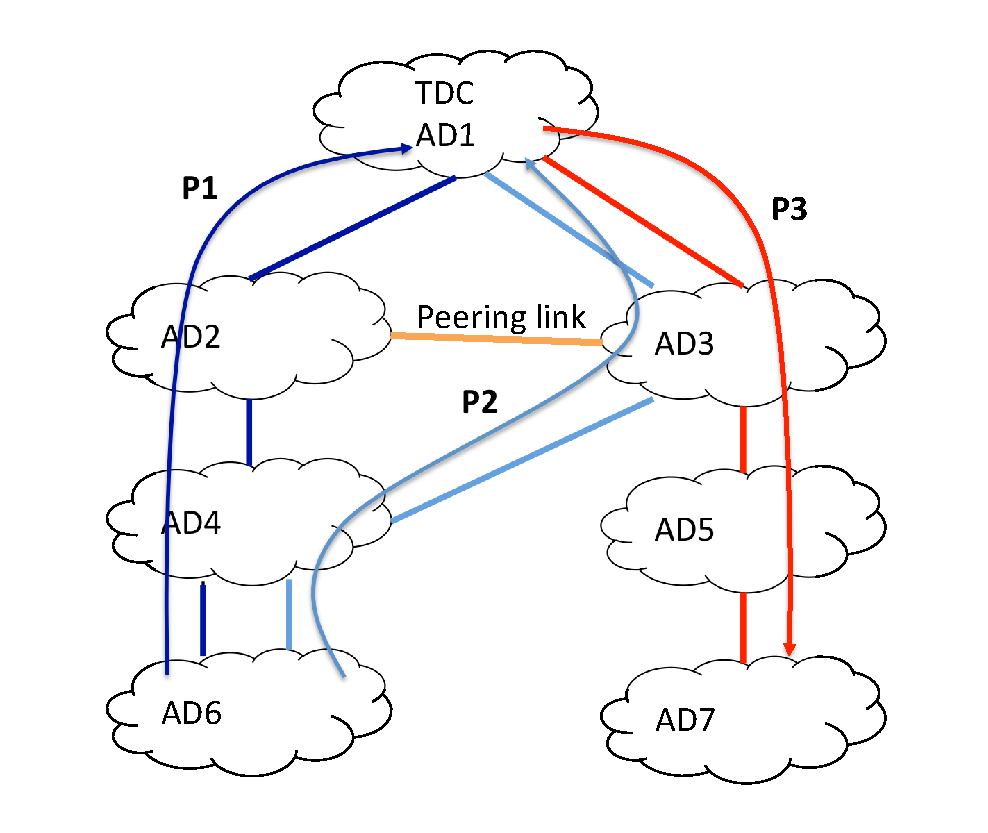
\includegraphics[width=.7\columnwidth]{./fig/pathjoin.eps}
\caption{Example: Path Joining.}~\label{fig:pathjoin}
\end{figure*}

\begin{figure*}[ht]
\centering
\mbox{\subfigure[Up-path Table]{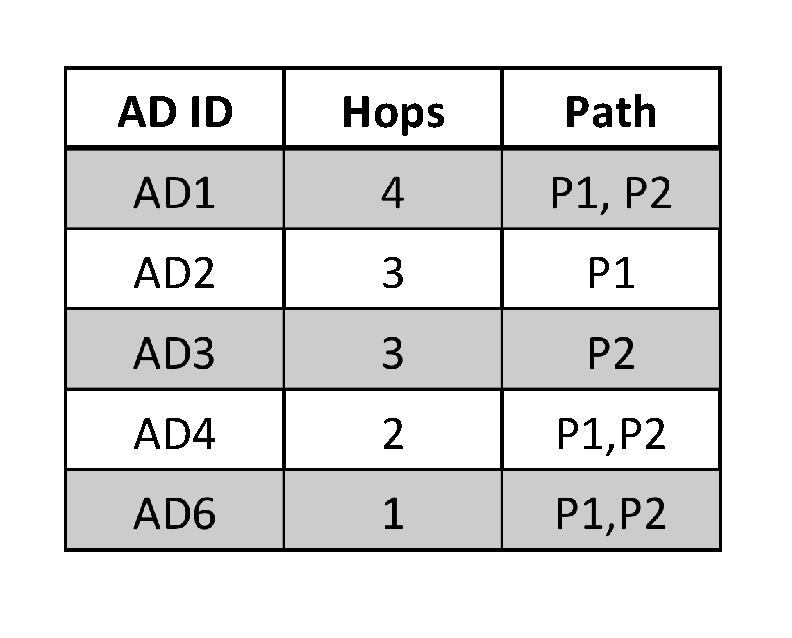
\includegraphics[scale=.5]{./fig/uppath_table.eps}}~\label{fig:uppath-table}\quad
\subfigure[Down-path Table]{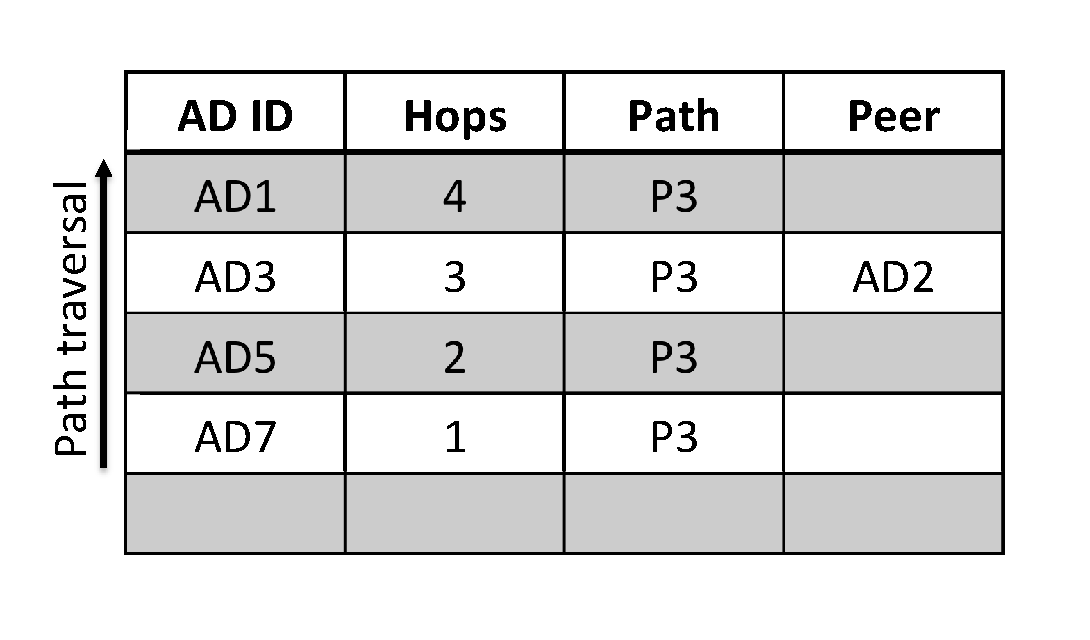
\includegraphics[scale=.5]{./fig/downpath_table.eps}}~\label{fig:downpath-table}}
\caption{Example: The up-path and the down-path tables for two up-paths (i.e., P1, P2) and a single down-path (P3) for Figure~\ref{fig:pathjoin}.}
\end{figure*}

In this section, we describe how to construct an end-to-end path using the up-paths and down-paths provided by the local \PS.

The local \PS has a large number of up-paths provided by the local \BS and a set of down-paths to a specific destination \AD provided by a \ISDC \PS.
An end-to-end path is constructed by joining an up-path and a down-path and is represented by a series of opaque fields preceded by SCION common header and two special opaque fields (i.e., up and down timestamps). Path joining can be performed either by the local \PS or by a client who wants to contruct a path. Path joining at a client is very simple as the client join all possible combination of up- and down-paths and select the best path among them. However, such brute-force joining is very inefficient if it is performed at the local \PS because (1) the \PS has a large number of up-paths and possibly many down-paths (if the \PS caches the down-paths of an \AD and reuse them until they expire, instead of using them once) and (2) each path may contain many peering links. In this case, joining all up- and down-paths incurs a huge overhead to the \PS. We resolve this issue by designing an efficent path joining algorithm below.

A half-path (either up- or down-path) consists of a series of ADs, where each AD is identified by its ADID and its ingress and egress interfaces. Hence, even if two paths contain the same series of ADs, they can differ if any one of the interface is not same. However, we do not distinguish a path by its timestamps.

Our algorithm finds a shortest path(s) in terms of \AD hops and consists of three parts, which are up-path table construction, down-path table construction, and path traversal.

\subsection{Up-path Table}
The up-path table consists of three field as Figure~\ref{fig:uppath-table}: ADID, Hops, and Path. ADID is the AD identifier, Hops is the distance from the endpoint AD, and Path is the pointer to the path (i.e., PCB) that contains the current ADID. Each field is identified by a unique ADID, hence if a path contains a unique AD, it creates a new entry. If an ADID already exsits in the table, there are three choices: (1) if the Hops of the current path is same as the one in the table, its pointer is added to the Path field; (2) if the Hops is less than the existing one, it replaces the current one; and (3) if the Hops is greater than the existing one, it is discarded. For example, in Figure~\ref{fig:pathjoin}, P1 consists of AD1,AD2,AD4, and AD6 and is filled into the up-path table in the reverse order of PCB propagation. P2 is added to the table in the same way, yet only AD3 creates a new entry since other ADs already exist in the table (hence P2 is added to the Path field of existing AD entry).

\subsection{Down-path Table}
The down-path table has another field, peer ADID, in addition to all fields in the up-path table. The peer ADID is used to construct an end-to-end path through a peering link. Since the relationship of a peering link is symmetric (i.e., if it appears the up-path, it should appear in the down-path, and vice versa), we only need to add this information either to the up-path table or to the down-path talbe. We add the peering information to the down-path table since the number of down-paths is smaller than that of up-paths, and the path construction starts from the down-path (hence it is more efficient to include it in the down-path table).

\subsection{Path Traversal}
With the up-path and the down-path tables, one can construct an end-to-end shortest path as follows.
\begin{enumerate}
\item Start from the endpoint \AD in the down-path table.
\item Find the same ADID staring from the endpoint (i.e., Hops == 1) \AD toward TDC \AD in the up-path table.
\item If the same ADID exists in the ADID field of the up-path table, the corresponding AD is the crossver \AD through which a shortcut path is constructed.
\item If the path-length of the shortcut path is less than the current minimum, replace the shortest-path list with the shortcut path.
\item If the path-legnth of the shortcut path is equal to the current minimum, add the shortcut path to the shortest-path list.
\item For each peer ADID in the current down-path entry, do 2-5 with the peer ADID. If a matching ADID is found in the up-path table, a shorcut path is constructed through a peering link between the ADID and the peer ADID.
\item Repeat 2 - 6 for all \ADs toward TDC \AD in the down-path table. 
\end{enumerate}

We note that an end-to-end path consists of a pair of up-path and down-path, hence is stored as a pair. We also note that if the Path field at the crossover \AD has multiple entries (e.g., up-path P1, and down-paths P2, P3), both paths are added to the shortest-path table (i.e., (P1,P2), (P1,P3)). We can set the maximum size of the shortest-path list (e.g., to $k$) and store the (first) k-shortest paths in order not to keep unnecessarily many paths.


\begin{comment}
Our solution is AD-level (turning point) search plus opaque-field path construction. The reason for this approach is as below. First, we should be aware that we are dealing three data structures at the same time -- path, AD and opaque-field. Each path contains several ADs and each AD on the path is represented by an opaque-field with ingress interface, egress interface and MAC. For a single AD, there may be several paths that cross it so it could map to more than one opaque-field. To increase algorithm efficiency in finding the turning point for shortest path search, we need to extract the most relevant information from the path-AD-OF data and hide irrelevant details. That is the idea of AD-level search. In this stage we only care about finding the AD-level turning point and we hope that we can construct the end-to-end path from this turning point. 
To support the idea of AD-level search, we designed a data structure called âœAD table❠as the up-path AD table example shows below.

AD6 is the source, AD7 is the destination and AD1 is the ISD core. Each entry corresponds to an AD on the path with a vector of pointers to the path it belongs. For shortest path search we only store the pointer of the path whose AD is closest to the source. For instance, letâ™s assume there is another path3 that is AD6-AD9-AD4-AD2-AD1. Only p3 to path3 will be added to the AD6 and AD9â™s path vector because the hop numbers from AD4, AD2, AD1 to AD6 (source) are all larger than the current hops. 
	Similarly the AD table for down-path is as below.


	The only difference here is that there is another column called peer AD vector indicating to which ADs the entry AD has peering links. Not including peer AD vector in up-path AD table avoids information redundancy. It also helps save search time to put peer AD vector in the down-path AD table since there are less down-paths than up-paths.
		The AD-level search for turning point is to go through each entry of down-path AD table. First we see if the AD in the entry belongs to the up-path AD table, if so this AD is a cross-over point and we calculate the sum of hops of these two entries and compare it with the lowest path hop number, if it is less than we mark the entry ADs. Then we see if the peers of the AD belongs to the up-path AD table, if so there is a peering link then we calculate the total hops and compare and if it has less hop we mark the two ADs. In the case below, the AD3 in down-path table and up-path AD table is a crossover point that corresponds to the shortest path with 3+3-1=5 hops.

		Having found the âœturning pointâ, we pick one path pointer p3 in AD3â™s path pointer vector in down-path AD table and p2 in AD3â™s path pointer vector in up-path AD table to construct the full path (end-to-end path). This is called opaque-field-level path construction. The full path is shown as below.
\end{comment}

  
\section{SCION Cryptographic Implementation}

Here we describe all cryptographic algorithms and implementation detail in SCION architecture. 

\subsection{pseudo random number generator}
We all know the pseudo random number generator (PRNG) is pretty hard to design especially
the generated numbers should fit in the a uniform distribution.
In SCION architecture, we leverage the PRNG provided by the crypto processor inside
the TPM (Trusted Platform Module).

\subsection{cryptographic hash}
As we known, previous legacy cryptographic hashes, such as MD5, SHA0, have been successfully attacked. %require refs
Even SHA1 has been proofed as weak under theoretical attacks. %require refs
Therefore, we choose SHA3 (Keccak) as our cryptographic hash algorithm in SCION architecture.
In practices, SHA3 still keep good software performance. According to the official released data, 
SHA3 could achieve around 12.5 cycles per byte on Intel Core 2 CPUs (SHA3 hash output is 512-bits). 

\subsection{key derivation function}
Not decided yet.

\subsection{message authentication code (MAC)}
%HMAC is based on SHA3 directly because we already select SHA3 as our hash algorithm.
%In contrast to HMAC-SHA1, HMAC-SHA3 does not need nested computation.
Need Discussion. We could use CBC-MAC based on AES-NI instruction set or SHA3.
AES-CBC-MAC has instruction advantage because intel i5/i7 processors support it.
The disadvantage is CBC-MAC is a nested construction.
Comparing to SHA3, HMAC based on SHA3 could be easily computed,
e.g., MAC of message $M$, $C$ = SHA3($K||M$) where $K$ is the symmetric key.
HMAC-SHA3 does not need any nested constructions.

\subsection{symmetric cipher}
We choose AES as the symmetric cipher because intel CPU processors support
AES-NI instruction set. AES-NI introduces powerful instructions, such as AESENC,
AESDEC for one round AES encryption and decryption. It also provides AESKEYGENASSIST
for key expansion in a fast fashion. By leveraging the AES-NI instruction set, we could
achieve better performance. We conduct a experience using intel AES-NI sample library
over an intel xeon processor; the result is given in Table~\ref{table:aesni_data}.

\begin{table*}[tb]
\centering
\caption{AES performance test over Intel Xeon E5640 Processor. We performed
AES CBC encryption/decryption on a 50MB file over multiple loops, 100 times.}
\label{table:aesni_data}
\begin{tabular}{|c|c|c|c|c|c|} \hline
key size  & Encryption & Decryption& Key Expansion & Encrypt Cost & Decrypt Cost\\ 
(bits)  & (sec) & (sec) & Enc/Dec(cycles) &  (cycle/byte)  & (cycle/byte) \\  \hline
128  &0.0785 & 0.0245 & 181.74/227.4 & 3.98 & 1.24 \\  \hline
192  &0.0912 & 0.0291 & 216.26/290.74 & 4.63 & 1.48 \\  \hline
256  &0.1056 & 0.0335 & 224.40/307.54 & 5.36 & 1.69 \\  \hline
\end{tabular}
\end{table*}

\subsection{asymmetric cipher}
For asymmetric key cipher, we select ECIES (Elliptic Curve Integrated Encryption Scheme)
because we try to get rid of the key exchange to generate the shared key between two parties,
e.g., ECDH (Elliptic Curve Diffie-Hellman). RSA-based encryption schemes, such like PKCS\#1, is
also not our candidate due to the size of cipher text and key pair. In order to provide
sufficient security, we should adopt RSA 2048-bit or higher to prevent well-known attacks.
For elliptic curve cryptography, we could choose several NIST-recommand curves over different
key size (See FIPS 186-3). To offer RSA 2048 bits security, we only need 224 bit elliptic curve
construction. ECIES already has several open source implementations, such as Crypto++.

\subsection{digital signature}
We need a description for Ed25519 and some experience data about it.

  \section{System Configuration}\label{sec:system-configuration}

\subsection{SCION Switch}
A SCION switch connects all SCION elements within an \AD to abstract intra-\AD communication. SCION defines a new inter-\AD routing architecture (including corresponding protocols), yet does not mandate any intra-\AD architecture. Hence, an \AD will be able to adopt SCION without changing the current internal forwarding/routing mechanisms. A SCION switch is a special element that virtualizes intra-\AD communication and can be replaced by intra-\AD forwarding/routing mechanisms in real operation.

All SCION elements such servers and border routers are assigned a unique AID and should be reached with their AID. A SCION switch simply maintains its port to an element's AID mapping to enables communication between elements. AID = 0xFFFFFFFFFFFFFFFF is reserved for broadcasting a message to all elements; e.g., server list announcement. A SCION switch constructs a map between an output port and the AID of the connected element to the port during initialization. Specifically, a SCION switch sends AID request messages (AID\_REQ) to all output ports and the connected elements reply with their own AID (AID\_REP). The SCION switch constructs a AID-to-port mapping table using the AID reply arrived at each port. Note that an input port does not need to be mapped to the connected element's AID since a switch does not write (and hence route) any packet to the port (i.e., read-only port).

\begin{figure}[ht]
\centering
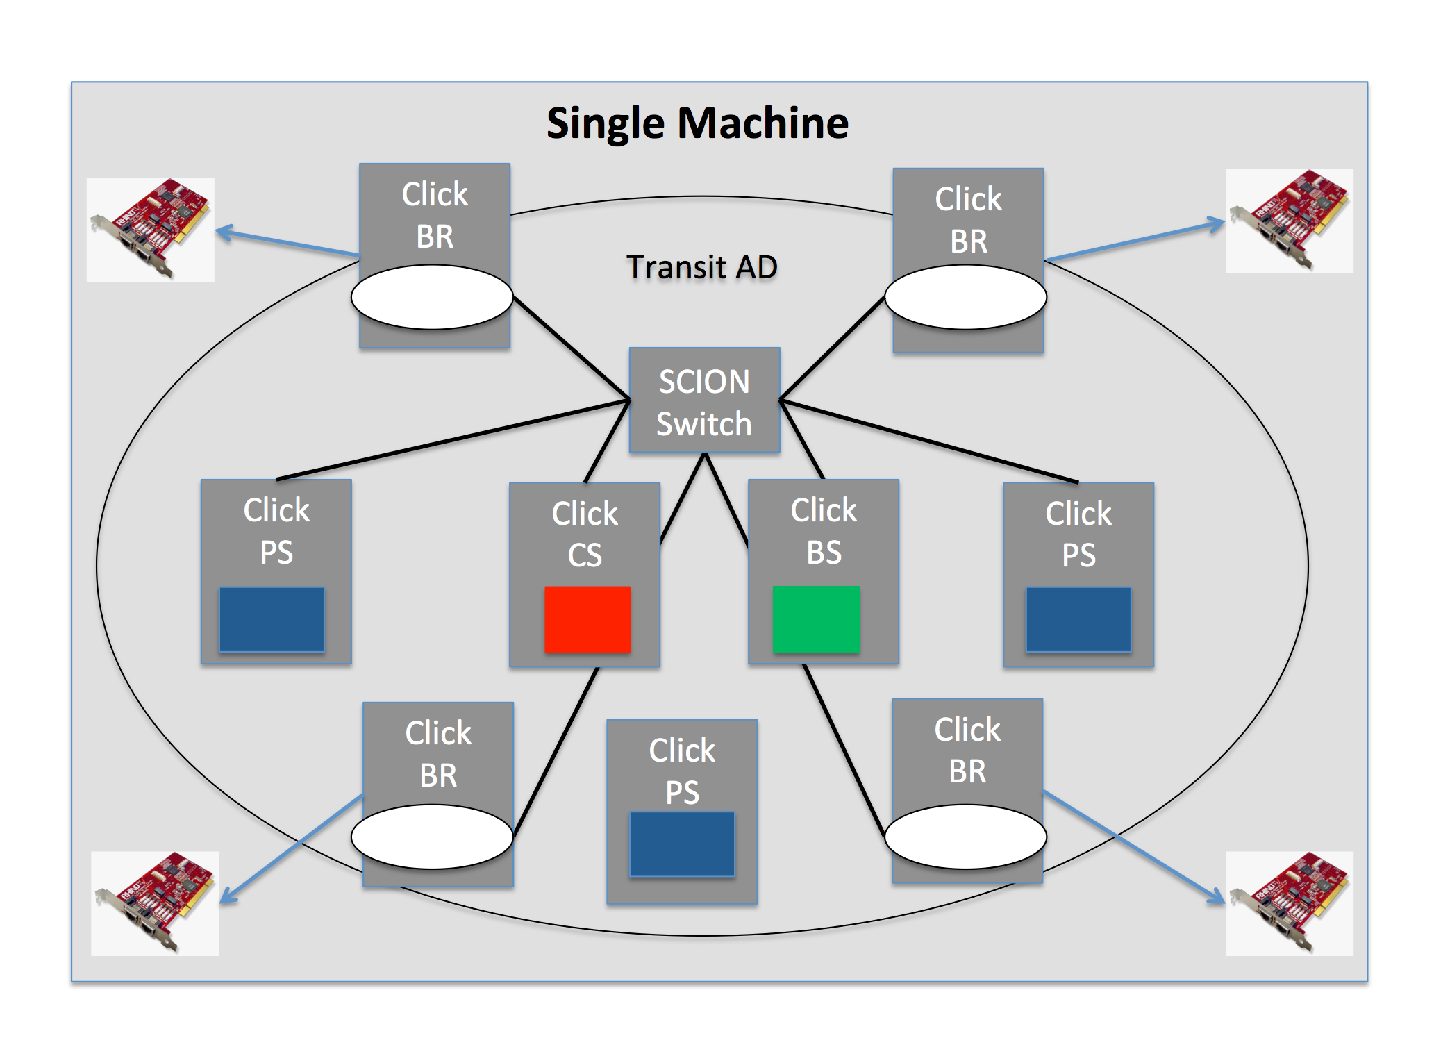
\includegraphics[width=.8\columnwidth]{./fig/configuration.eps}
\caption{Configuration. All elements are connected through a SCION switch.\newline
BR: Border Router, CS: Certificate Server, BS: Beacon Server, PS: Path Server}\label{fig:configuration}
\end{figure}

Figure~\ref{fig:configuration} illustrates how elements are interconnected through a SCION switch within an \AD. In this example, border routers connect to other \ADs through an NIC. Yet, multiple \ADs can be configured in a single machine or each \AD can be configured in a separate virtual machine.


\subsection{Click Configuration File}
Currently, we have five types of Click elements, which are Certificate Server, Beacon Server, Path Server, Border Router and SCION Switch.  
Each element is configured in a .click file (i.e., a click router configuration file) as follows.

Note: every element has its own (object) name for .click file generation. This name is meaningful in .click file.

\begin{itemize}
\item Certificate Server: AID, Address Type, Address, Configuration File, Topology File, RoT File.
\item Beacon Server: AID, Address Type, Address, Configuration File, Topology File, RoT File.
\item Path Server:AID, Address Type, Address, Configuration File, Topology File.
\item Border Router:AID, Address Type, Address, Configuration File, Topology File.
\item SCION Switch:
\end{itemize}

\subsection{SCION Configuration File}
In addition to the basic configuration parameters, more detailed parameters specific to each element are defined in .conf file. In other words, each element has its own configuration file and intializes itself with this file. The configuartion paratmers of individual elements are shown below.

\begin{itemize}
\item Certificate Server: ADID, TDID, RegTime, PropTime, Log Level, Private Key File, Certificate File, Master OFG Key, Master AD Key.
\item Beacon Server: ADID, TDID, RegTime, PropTime, Log Level, Private Key File, Certificate File, Master OFG Key, Master AD Key, PCB Queue Size, Number of Registered Path, Number of Up Path, Register Path (bool).
\item Path Server: Path Server Queue Size,  Log File.
\item Border Router: Queue Size, Log File, Interfaces, Master OFG Key, Master AD Key. 
\item SCION Switch:
\end{itemize}


\begin{comment}
\subsection{Interconnect}
\begin{itemize}
\item Intra-machine
\item Inter-machine
\end{itemize}
\end{comment}


  \chapter{Examples}


  % \input{Acknowledgments}

  \bibliographystyle{plain}
  \bibliography{src/bib}
  \nocite{ZHHCPA2011}

  \appendix
  \chapter{Further Reading}

This section provides an overview of the scientific publications related to SCION.
\todoRR{need longer abstract/descriptions here.}

\begin{itemize}

\item \textbf{SCION: Scalability, Control, and Isolation on Next-Generation Networks}~\cite{ZHHCPA2011}\\
\textit{X. Zhang, H. Hsiao, G. Hasker, H. Chan, A. Perrig, and D. Andersen} \\
{\footnotesize Proceedings of the 32nd IEEE Symposium on Security and Privacy (Oakland), 2011.}

This work describes the initial SCION architecture...


\item \textbf{LAP: Lightweight Anonymity and Privacy}~\cite{HKPYNGM2012}\\
\textit{H. Hsiao, T. Kim, A. Perrig, A. Yamada, S. Nelson, M. Gruteser, and W. Meng} \\
{\footnotesize Proceedings of the 33rd IEEE Symposium on Security and Privacy (Oakland), 2012.}


\item \textbf{STRIDE: Sanctuary Trail – Refuge from Internet DDoS Entrapment}~\cite{HKYZLGP2013}\\
\textit{H. Hsiao, T. Kim, S. Yoo, X. Zhang, S. Lee, V. Gligor, and A. Perrig} \\
{\footnotesize ASIACCS~'13: Proceedings of the 8th ACM Symposium on Information, Computer and Communications Security, 2013.}


\item \textbf{Accountable Key Infrastructure (AKI): A Proposal for a Public-Key Validation Infrastructure}~\cite{KHPJG2013}\\
\textit{T. Kim, L. Huang, A. Perrig, C. Jackson, and V. Gligor} \\
{\footnotesize WWW~'13: Proceedings of the 22nd International World Wide Web Conference, 2013.}




\end{itemize}



  % Glossary and Abbreviation List.

% Syntax:

%    \gitem{Title}{Description}

% Creates an entry of the form Title --> Description.
% This list of items is automatically sorted by title.
% When inserting an entry, don't care about its position.

% When you introduce an abbreviated entry, e.g., Core Beacon
% Server (CBS), then please add below your \gitem entry an
% abbreviation entry as follows:

%    \abbrev{CBS}{Core Beacon Server}

% This entry will appear in the abbreviation list (behind
% the glossary) and in the index with both abbrevation and
% non-abbreviated string.

% If you want to add a manual entry to the index, please
% use the additional optional argument as follows:

%    \gitem[Keyword]{Title}{Description}

% The keyword string will appear in the index and point
% to the page where the glossary entry appears.
% Be careful when using the optional index keyword in
% conjunction with the \abbrev command. Both add an index
% entry. You should omit the index keyword in case you
% use \abbrev.



\begin{SCIONglossary}

% Raphael

\gitem[path server]{Path Server}{Facility within an isolation domain
where end hosts register their up- and down-paths. End hosts can
query path servers in order to obtain valid paths do a destination.}

\gitem{Isolation Domain (ISD)}{Hierarchical and self-contained unit
with own jurisdiction in which a number of ASes are located.}

\abbrev{ISD}{Isolation Domain}

\gitem[half-path]{Half-Path}{Up-path from an end entity to the ISD
core, or down-path from the ISD core to an end entity.}

\gitem[inter-domain path]{Inter-Domain Path}{Path between two ADs
that are located in two different ISD cores.}

\gitem[end-to-end path]{End-to-End Path}{Stitched path between two
end entities, typically consisting of three paths: an up-path, an
inter-domain path, and a down-path.}

% Pawel.

\gitem{Core Beacon Server (CBS)}{Facility within a core AD that
initiates the PCB construction.}

\abbrev{CBS}{Core Beacon Server}

\gitem{Local Beacon Server (LBS)}{Facility within a non-core AD that
receives all Path Construction Beacons (PCBs) from the provider ADs.
At every propagation period, an LBS performs two steps: (a) it
selects $k$ PCBs and registers them as down-paths at the Core Path
Server (CPS), and (b) it selects $k$ PCBs and registers them as
up-paths at the Local Path Server (LPS). Selection criteria for down-
and up-paths may differ.}

\abbrev{LBS}{Local Beacon Server}

\gitem{Path Construction Beacon (PCB)}{to be done}

\abbrev{PCB}{Path Construction Beacon}

\gitem{Core Path Server (CPS)}{Facility within a core AD, where
non-core ADs (within a given ISD) register their down-paths. The CPS also
serves down-path requests by translating a requested (ISD, AD) pair to
an appropriate down-path.}

\abbrev{CPS}{Core Path Server}

\gitem{Local Path Server (LPS)}{Facility within a non-core AD, where
Local Beacon Servers register their up-paths. End hosts can query an
LPS in order to obtain valid up- and down-paths to a destination.
Down-paths are obtained through querying the Core Path Server (CPS)
or using cached results.}

\abbrev{LPS}{Local Path Server}

% Cristina.

\gitem[static path]{Static Path}{Long-lived, low-bandwidth
reservation on top of half-paths. Static paths are initiated by leaf
ADs and are used in SIBRA for two purposes: (1) as a building block
for priority paths: to guarantee availability during connection
setup, and to perform weighted bandwidth reservation, and (2) to
provide communication guarantees for low-bandwidth traffic, e.g.
control traffic.}

\gitem[priority path]{Priority Path}{Short-lived, high-bandwidth
reservation on top of end-to-end paths, i.e., up-path, inter-domain
path, and down-path. Priority paths are initiated by end hosts in
SIBRA. They are only valid on the order of tens of seconds, and thus
needs to be continuously renewed.}

\gitem{Reservation Token (RT)}{Cryptographically authenticated token
that enables the usage of SIBRA bandwidth reservations. RTs are
enriched opaque fields that encode the amount of bandwidth and the
validity of an AD's bandwidth reservation for a specific flow.}

\abbrev{RT}{Reservation Token}

\gitem[DRKey protocol]{DRKey Protocol}{Protocol to enable routers
$R_i$ on a source-specified path $\langle S, R_1, \allowbreak R_2,
\ldots, D\rangle$ to set up on-the-fly shared keys with source $S$
and destination $D$. DRKey protocols enable routers to re-derive keys
on the fly when needed, thus avoiding the need of per-flow state on
routers.}


\gitem[DRKey session]{DRKey Session}{Session that identifies the
packets sent by a source $S$ to a destination $D$ on the same path,
during a certain period of time. A DRKey session is typically
associated with a flow that travels the same network path, such as a
TCP flow in SCION.}

\gitem[Retroactive-DRKey]{Retroactive-DRKey}{DRKey protocol that
enables entities on the path to set up shared keys at any time after
the first packet in a DRKey session reaches the destination.
Retroactive-DRKey hides the source's intention to set up shared keys
with the routers on the path, preventing coward attacks.}


\end{SCIONglossary}


  
\chapter{DTD definition for configuration files}
Here we define two DTD definition for two xml files for configuration.

\section{RoT file DTD: rot.dtd}
\label{sec:rotdtd}

%definietion for dtd
\begin{verbatim}
<!DOCTYPE ROT [
<!ELEMENT ROT (header,coreADs,signatures)>
<!ELEMENT header (version,issueDate,expireDate,policyNumber,ISDID,policyThreshold,certificateThreshold)>
<!ELEMENT version (#PCDATA)>
<!ELEMENT issueDate (#PCDATA)>
<!ELEMENT expireDate (#PCDATA)>
<!ELEMENT policyNumber (#PCDATA)>
<!ELEMENT ISDID (#PCDATA)>
<!ELEMENT policyThreshold (#PCDATA)>
<!ELEMENT certificateThreshold (#PCDATA)>
<!ELEMENT coreADs (coreAD+)>
<!ELEMENT signatures (coreAD+)>
<!ELEMENT coreAD (AID,(cert|sign))>
<!ELEMENT AID (#PCDATA)>
<!ELEMENT cert (#PCDATA)>
<!ELEMENT sign (#PCDATA)>
]>
\end{verbatim}

This dtd indicates that produceed rot xml file should follow the rules.
\begin{enumerate}
	\item The document root element is ROT.
	\item Element ROT has three child elements, header, coreADS, and signatures which must occur once, and only once.
	\item Element header has four child elements as well. Similary, they are only allowed to define once, and only once.
	\item Elemenet coreADs and signatures should has at least one child element coreAD.
	\item Element coreAD could be contain AID element and either cert or sign element.
\end{enumerate}

\begin{SaveVerbatim}{RotSample}
<?xml version="1.0" standalone="no" ?>
<!DOCTYPE document SYSTEM "rot.dtd">
<ROT>
	<header>
		<version>0x0001</version>
		<issueDate>Fir Jul 6 15:44:25 EDT 2012</issueDate>
		<expireDate>Fir Jul 6 15:44:25 EDT 2013</expireDate>
		<policyNumber>2</policyNumber>
		<ISDID>12345</ISDID>
		<policyThreshold>2</policyThreshold>
		<certificateThreshold>2</certificateThreshold>
	</header>
	<coreADs>
		<coreAD>
			<AID>321</AID>
			<cert>TESTBUB</cert>
		</coreAD>
		<coreAD>
			<AID>322</AID>
			<cert>TESTBUB</cert>
		</coreAD>
	</coreADs>
	<signatures>
		<coreAD>
			<AID>321</AID>
			<sign>TESTSIGNATURE</sign>
		</coreAD>
		<coreAD>
			<AID>321</AID>
			<sign>TESTSIGNATURE</sign>
		</coreAD>
	</signatures>
</ROT>
\end{SaveVerbatim}

Sample RoT xml file could be defined as follows:

\BUseVerbatim[fontsize=\footnotesize]{RotSample}

\section{Topology file DTD: topology.dtd}
\label{sec:topologydtd}

%definietion for dtd
\begin{verbatim}
<!DOCTYPE Topology [
<!ELEMENT Topology (header,Servers,BorderRouters,Gateways,Signature)>
<!ELEMENT header (version,issueDate,ISDID,ADID)>
<!ELEMENT version (#PCDATA)>
<!ELEMENT issueDate (#PCDATA)>
<!ELEMENT ISDID (#PCDATA)>
<!ELEMENT ADID (#PCDATA)>
<!ELEMENT Servers (BeaconServer,PathServer,CertificateServer)>
<!ELEMENT BeaconServer (AID)>
<!ELEMENT PathServer (AID)>
<!ELEMENT CertificateServer (AID)>
<!ELEMENT BorderRouters (Router+)>
<!ELEMENT Router (AID,Interface+)>
<!ELEMENT Interface (IFID,NeighborAD,NeighborType)>
<!ELEMENT IFID (#PCDATA)>
<!ELEMENT NeighborAD (#PCDATA)>
<!ELEMENT NeighborType (#PCDATA)>
<!ELEMENT Gateways (Gateway+)>
<!ELEMENT Gateway (AID,Protocol)>
<!ELEMENT AID (#PCDATA)>
<!ELEMENT Protocol (#PCDATA)>
<!ELEMENT Signature (#PCDATA)>
]>
\end{verbatim}

%This dtd indicates that produceed rot xml file should follow the rules.
%\begin{enumerate}
%	\item The document root element is ROT.
%	\item Element ROT has three child elements, header, coreADS, and signatures which must occur once, and only once.
%	\item Element header has four child elements as well. Similary, they are only allowed to define once, and only once.
%	\item Elemenet coreADs should has at least one child element coreAD.
%	\item Element signature has an attribute called AID which is a required field.
%\end{enumerate}

\begin{SaveVerbatim}{TopoSample}
<?xml version="1.0" standalone="no" ?>
<!DOCTYPE document SYSTEM "topology.dtd">
<Topology>
	<header>
		<version>0x0001</version>
		<issueDate>Fir Jul 6 15:44:25 EDT 2012</issueDate>
		<ISDID>54321</ISDID>
		<ADID>12345</ADID>
	</header>
	<Servers>
		<BeaconServer><AID>12345-1</AID></BeaconServer>
		<PathServer><AID>12345-2</AID></PathServer>
		<CertificateServer><AID>12345-3</AID></CertificateServer>
	</Servers>
	<BorderRouters>
		<Router>	
			<AID>12345-4</AID>
			<Interface>
				<IFID>0xef123456</IFID>
				<NeighborAD>12346</NeighborAD>
				<NeighborType>0x0001</NeighborType>
			</Interface>
			<Interface>
				<IFID>0xef123457</IFID>
				<NeighborAD>12347</NeighborAD>
				<NeighborType>0x0001</NeighborType>
			</Interface>
			<Interface>
				<IFID>0xef123458</IFID>
				<NeighborAD>12348</NeighborAD>
				<NeighborType>0x0001</NeighborType>
			</Interface>
		</Router>
	</BorderRouters>
	<Gateways>
		<Gateway>
			<AID>12345-5</AID>
			<Protocol>ICMP</Protocol>
		</Gateway>
	</Gateways>
	<Signature>TESTSIGNATURE</Signature>
</Topology>
\end{SaveVerbatim}

Sample Topology xml file could be defined as follows:

\BUseVerbatim[fontsize=\footnotesize]{RotSample}

  \printindex

\end{document}




%%% Local Variables: 
%%% mode: latex
%%% TeX-master: t
%%% End: 
